
\begin{firekeeper}{}
    \begin{wrapfigure}{r}{0.165\textwidth}
        \vspace{-2cm}
        \centering
        \hspace{-3cm}
        \raisebox{-1.65cm}{%      % 视觉上向上移动 0.5cm (负数则向下)
            \hspace*{0.10cm}%   % 视觉上向左移动 0.5cm (正数则向右)
            \scalebox{1.25}{%   % 视觉上缩放 1.25 倍
                
\includegraphics[width=0.30\textwidth]{firekeeper.png}%
            }%
        }
    \end{wrapfigure}

    \hspace*{1.6em} 亲爱的余火大人，恭喜您成功觐见了王者---树与二叉树，并从那古老而伟大的王座之前，获得了属于王的力量。
    
    \hspace*{1.6em} 接下来，您将踏入的区域名为万象之都。
    在那座古都深处，沉睡着一位孤独的王者。他无声地注视着世间万物的交织与离散，等待着命运的召唤。他的名字便是——图。相传这位孤独的王者正是那雾的彼端的初王之子。
    CoreLoop已在此地刻下曾经发生在雾的彼端，那名为罗德尔的传奇王国的故事，它将伴随您走完本区域的旅程。\\



    \hspace*{1.6em} 余火大人啊……您未曾得到火焰的指引，却仍凭着自己的意志，一步一步地穿越荆棘与黑暗，走到了这里……
    我曾无数次望见，您身上的伤口才刚刚愈合，转眼间却又添上了新的伤痕。可即便如此，您依旧默默地站起身来，
    继续走向那未知的远方。我也曾在寂静的深夜，看见您独自仰望那片遥远的星空，仿佛有千言万语萦绕心头。
    
    \hspace*{1.6em} 您从不曾向任何人诉说自己的苦楚，也不曾让泪水从眼中落下……可是，亲爱的余火大人
    ……我多么希望，至少在我的面前，您不必如此坚强。

    \hspace*{1.6em} 倘若这漫长的旅途令您感到疲惫，便请稍稍停下脚步吧。哪怕只有片刻也好，请让我陪伴在您的身旁，让您不必独自面对这无边的黑暗。
    因为对我而言，您并非只是那位不断前行的思渡者。\\

    \hspace*{1.6em} 您也是……我由衷牵挂着的人啊。
\end{firekeeper}

\chapter{图}

深夜，王都的钟声突然响起。

来自边境的信使带来了一个令人不安的消息：早已叛国的碎片君王们正带着大批军队向王国腹地推进，预计将于数月后抵达。国王立即召集所有军事指挥官，要求在天亮前制定出一套防御
方案。

王国境内分布着许多城镇、要塞、仓库等据点，它们通过道路相互连接。然而，道路的长短各不相同，并且有些需要穿梭险峻的山脉，有些需要横跨湍急的河流，还有一些因年久失修，早已
无法通行。

\begin{center}
    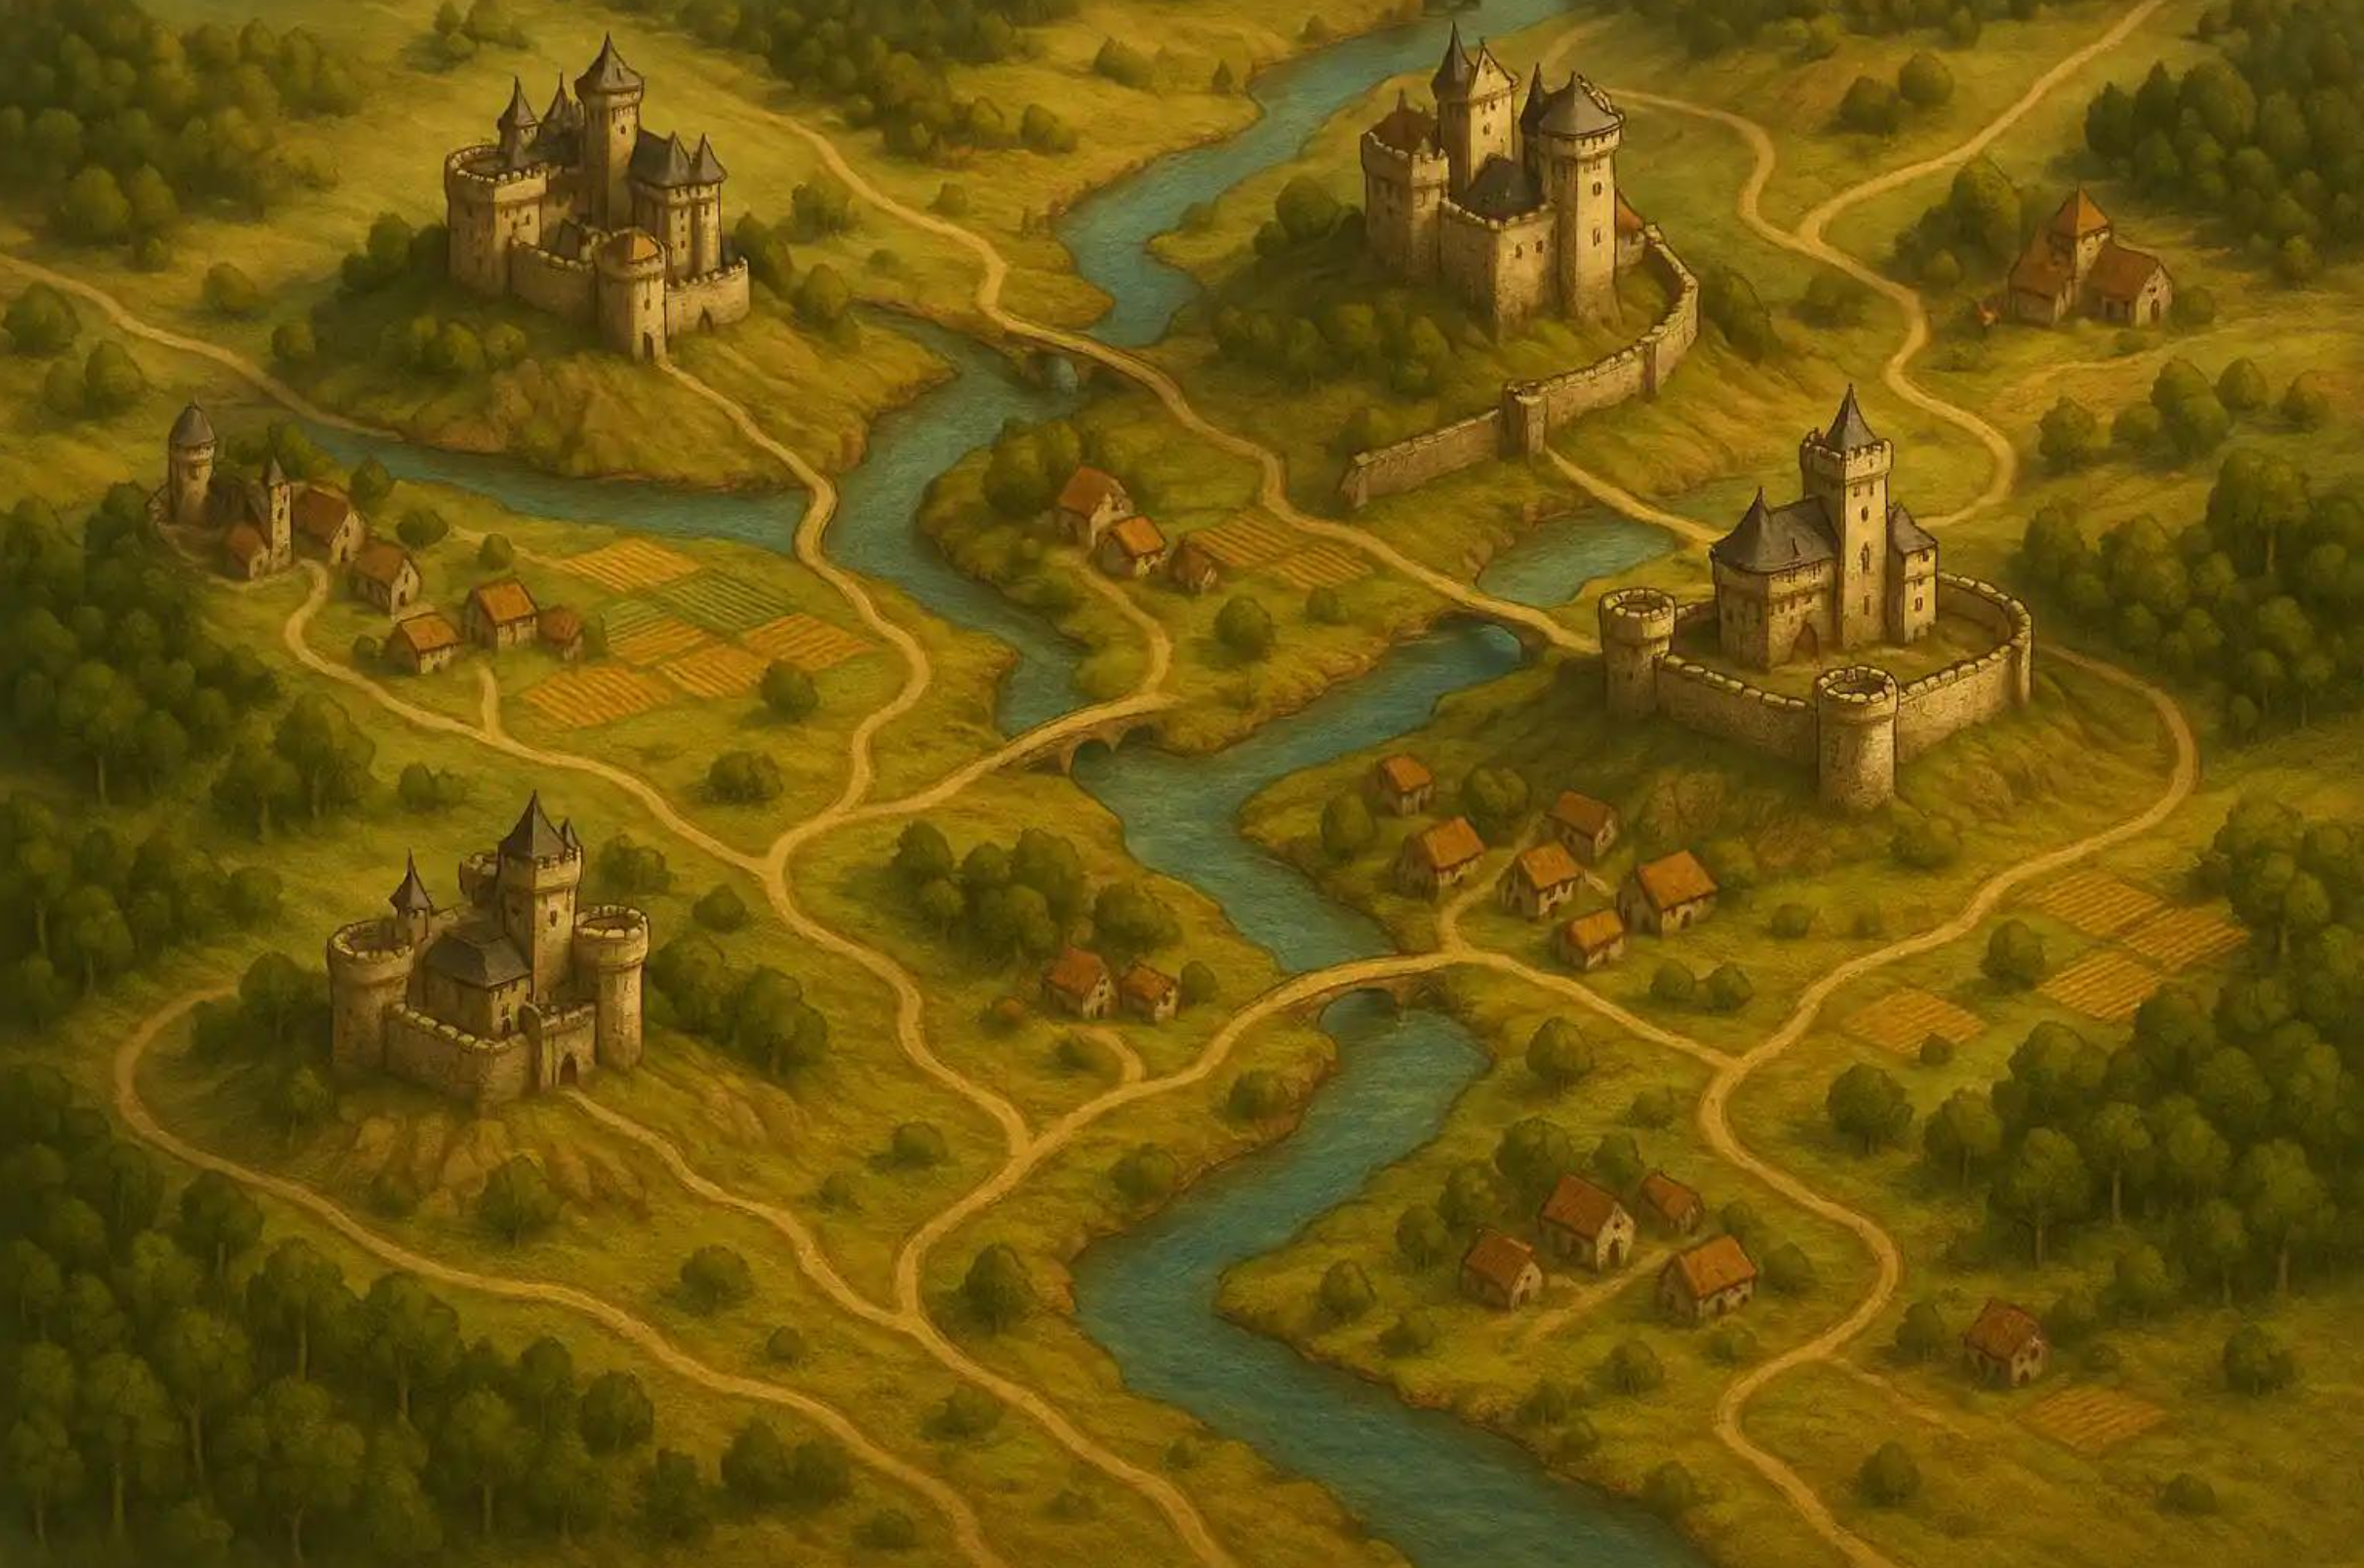
\includegraphics[width=0.95\textwidth]{assets/pics_and_ppts/ch5/王国.png}
\end{center}

如何快速确定哪些据点依然互相连通？若某个军事要点来犯，从首都派出军队，走哪条路能以最快速度到达？如何最优地铺设通信电线，以连接所有城镇？

......

时间正在飞速流逝，而摆在指挥官们面前的，是城镇、道路与错综复杂的连接关系。\\

经过不懈努力，指挥官们制定出了一套行之有效的防御模型。最终，入侵者被尽数驱逐，王国重归安宁。而这套曾经帮助王国渡过危机的模型，并未随着战争的结束而被
遗忘。相反，王国的后来者在此基础上不断探索、推演与完善，逐渐建立起一套严谨而完整的理论体系。虽然以上内容都是古老的传闻，但思渡者啊，在这片大陆上你看到的都并非虚妄。
在你觐见王者的途中，这段古老的传说将伴随你一同前行。\\



经过讨论，指挥官们决定将王国建模为一个\term{图}。他们将王国中的城镇、要塞等据点作为图的\term{顶点}，将据点之间的道路作为\term{边}。


\begin{definitionbox}
    图（Graph）是一种由\term{顶点}集合和顶点之间的\term{边}集合组成的数据结构，通常记为 \(G=(V,E)\)。其中，\(V\) 是有穷非空的顶点集合，\(E\) 是表示顶点之间关系的边集合。
    根据边是否具有方向，图可分为\term{无向图}和\term{有向图}：无向图中的边表示两个顶点之间不区分方向的关系，有向图中的边则表示从一个顶点指向另一个顶点的关系。
\end{definitionbox}


在第一章中（\bookmarkref{bookmark:waypoint-5}{waypoint-5}）我们曾经提到小队队员之间好感度的关系。更现实的情况是A对B的好感度与B对A的好感度并不相同，
这时就要使用\term{有向图}，来描述这种从一个顶点指向另一个顶点这种有方向的关系。比如邪念对银心好感度是5，而银心对邪念的好感度是8：

\begin{bulk}
\begin{center}
\begin{tikzpicture}
% 节点
\node[graphnode] (A) {邪念};
\node[graphnode] (B) [right=2cm of A] {银心};
\node[graphnode] (C) [below=1.5cm of A] {甘尔};
\node[graphnode] (D) [below=1.5cm of B] {张三};

% 有向边 + 权值
\draw[->] (A) to[bend left=15] node[above] {5} (B);
\draw[->] (B) to[bend left=15] node[below] {8} (A);

\draw[->] (A) -- node[left] {2} (C);
\draw[->] (A) -- node[right] {8} (D);
\draw[->] (B) -- node[right] {3} (D);
\draw[->] (C) -- node[below] {6} (D);
\end{tikzpicture}
\end{center}
\end{bulk}

王国的指挥官们认为，据点之间的道路若存在，则一定是可以双向通行的，因此他们使用\term{无向图}来描述王国。
为方便交流，他们对无向图做了如下约定：
\begin{enumerate}
    \item 将某顶点v的\term{度}定义为依附于顶点v的边的数量；
    \item 在无向图G中，若顶点v和顶点w之间有路径存在，则称这两个顶点是\term{连通的}。若图G中任意两个顶点都是连通的，则称图G为\term{连通图}，否则
    称为\term{非连通图}。无向图中的一个极大连通子图称为一个\term{连通分量}，孤立顶点被认为是一个连通分量。
    \item 由于无向图中边是双向的，因此一条边既可以看作出边，也可以看作入边。
\end{enumerate}
王国的后来者对类似的概念，在有向图上做了如下约定：
\begin{enumerate}
    \item 有向图中，某顶点v的度分为\term{入度}和\term{出度}。\term{入度}是“进来到该顶点的边数”，即以顶点v为终点的有向边的数量，而\term{出度}是
    “从该顶点出去的边数”，即以顶点v为起点的有向边的数量。顶点的出度和入度之和称为顶点的\term{度}。
    \item 在有向图G中，若从顶点v到w，以及从w到v之间都有路径，则称这两个顶点是\term{强连通的}。若图中任意一对顶点都是强连通的，则称该图为\term{强连通图}。
    类似地，有向图中的一个极大强连通子图称为一个\term{强连通分量}，孤立顶点被认为是一个强连通分量。
\end{enumerate}
连通分量和强连通分量通常也被称为\term{连通块}。

为加深记忆，指挥官们以如图\ref{fig:图的基本概念}的例子进行了一番交流：$G_1$是一个有5个顶点、4条边的图，由于它存在两个顶点不连通（如D与A），
因此它是一个非连通图；由ABC及连通它们的边$e_1$、$e_2$、$e_3$所构成的\term{子图}，是图$G_1$的一个连通分量，同理D、E及$e_4$也构成了一个连通分量。
\begin{figure}[htbp]
    \centering
    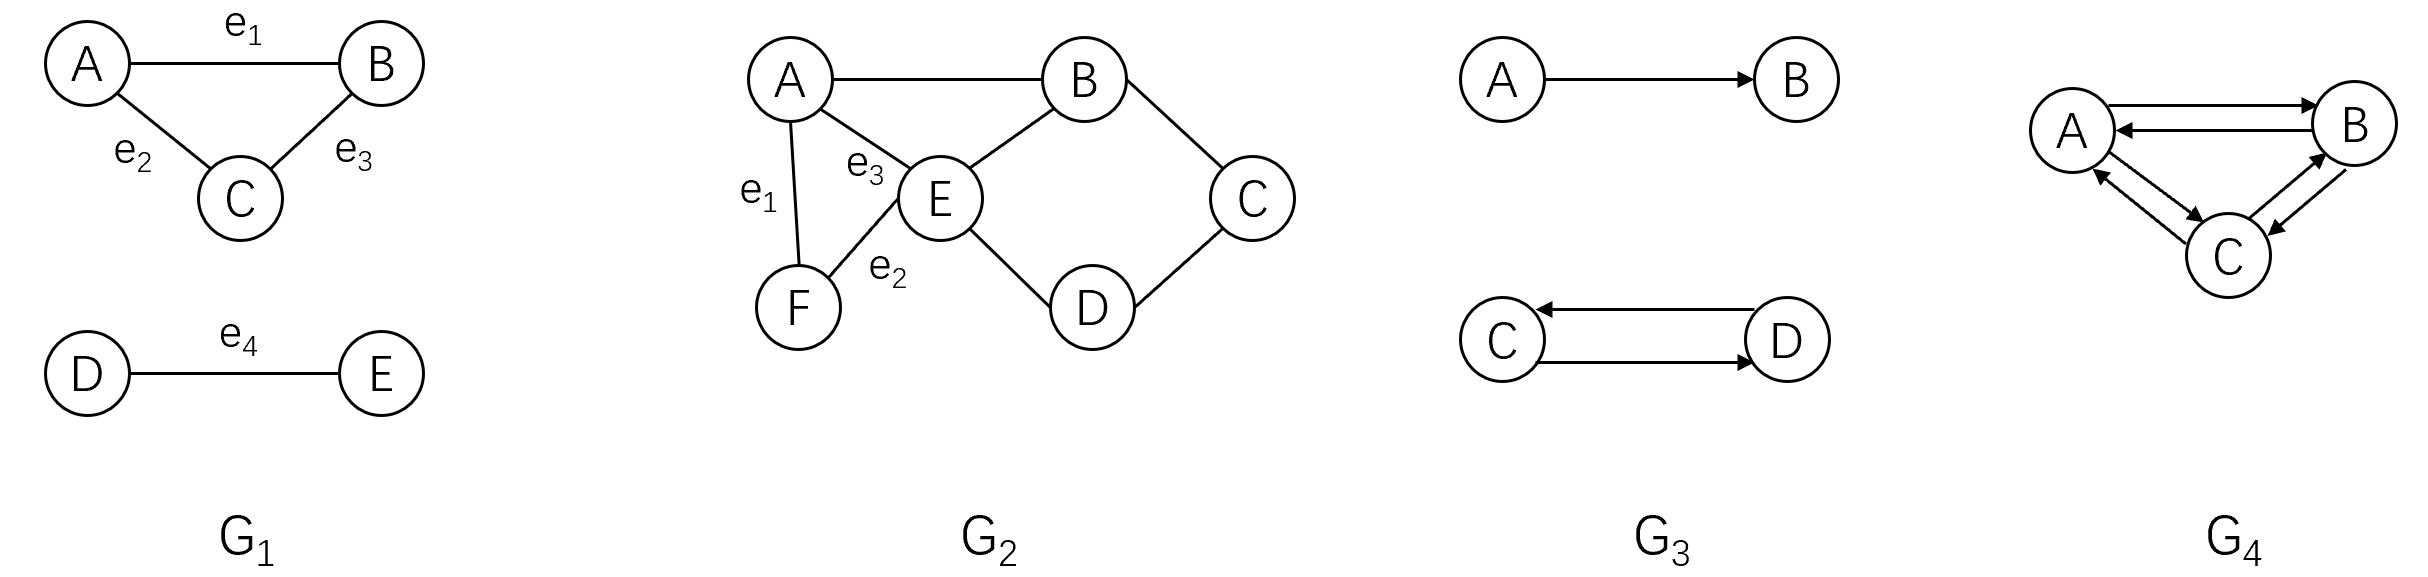
\includegraphics[width=0.98\textwidth]{assets/pics_and_ppts/ch5/图的基本概念.png}
    \caption{}
    \label{fig:图的基本概念}
\end{figure}

图$G_2$中，A、E、F及$e_1$、$e_2$、$e_3$构成的子图不能称为一个连通分量，因为它不是\textbf{极大}的。
\begin{intuitionbox}
    \term{极大连通子图}是指：在一个无向图中，不能再加入原图中的其他顶点及相关边而保持连通性的连通子图。有向图中\term{极大强连通子图}的概念类似。
\end{intuitionbox}
图$G_2$是一个连通图，因为任何两个顶点之间都有路径。图$G_2$中，顶点A、B的度为3，顶点E的度为4。

图$G_3$是一个有四个顶点、三条有向边的有向图。A的出度为1，入度为0；C、D的出度为1，入度为1。显然图$G_3$不是强连通图。注意：由于B到A不存在路径，
因此顶点A与B并非强连通。但该图并非只有一个强连通分量，而是有如下的三个：
\begin{center}
    
\includegraphics[width=0.42\textwidth]{assets/pics_and_ppts/ch5/图G3的三个强连通分量.png}
\end{center}

图$G_4$是一个强连通图，顶点A、B、C的出度和入度均为2；该图只有一个强连通分量，就是它自身。\\

根据实际应用的不同，顶点和边可能会携带一些信息，通常将边上的某种量化属性称为\term{边权}。如，指挥官们可能将顶点信息和边的信息分别用如下结构记录：

\begin{cppcode}
    struct VertexInfo {     // 顶点携带的信息
        char* name; // 据点的名字
        int weight; // 该据点的战略价值（重要性）
        //...
    };

    struct EdgeInfo {    // 边携带的信息
        int weight;     // 边权，可能是两据点间行军需要的时间，也可能是两据点间铺设通信电线需要的花费等等
    }
\end{cppcode}
这种边上带权的图称为\term{带权图}。绝大多数场景下，边只需表示顶点之间是否存在连接，或者额外记录一个权值，就足以解决实际问题。因此我们主要讨论这两种情况。
对于确实需要利用边的其他属性或更复杂信息的应用场景，我们再根据具体问题进行说明。

王国的城镇、要塞等据点成百上千，道路错综复杂。因此，指挥官们决定将建模输入他们的信息系统来解决问题。

\section{图的存储}
要存储一个由N个顶点，M条边构成的图，就需要存储所有顶点的信息、明确“哪些顶点之间存在边”以及存储这些边的权值。
要存储这N个顶点的信息非常简单，只需要一个数组即可：
\begin{cppcode}
    VertexInfo v[N];
\end{cppcode}
那么如何存储边与顶点的关系，以及边上携带的信息？经过研究，两位聪明的指挥官\uline{格佛莱}和\uline{麦丽凯}分别提出了两种策略。

\subsection{邻接矩阵}
\uline{格佛莱}指出，若将N个顶点编号为0到N-1，则通过一个矩阵（二维数组）：
\begin{bulk}
    \begin{center}
        int AdjM[N][N]; // Adjacency Matrix
    \end{center}
\end{bulk}
就可以明确“哪些顶点之间存在边”，以及这些边的权值是多少。例如若AdjM[0][2]的值是7，说明存在一条0号顶点到2号顶点的边，并且权值是7。显然对于无向图，AdjM[i][j]
和AdjM[j][i]的值一定是相等的，因此无向图的邻接矩阵一定是一个对称矩阵。而对于有向图，AdjM[i][j]和AdjM[j][i]可以分别表示i到j以及j到i是否
存在边、权值是多少。若边不存在，可以用一个在此场景无意义的数表示权值，如0、-1或正无穷等。

对于无权图，则无需记录边的权值，因此简单地用0、1表示边是否存在即可。

\begin{insightbox}
    CoreLoop提示：若在你的应用场景下，-1，0，负无穷、正无穷等都是可能存在的有意义边权，则可以在边的信息中加入一个bool值，标识这条边是否存在。\\
    \begin{center}
        EdgeInfo AdjM[N][N];    // EdgeInfo中包含一个 bool 变量。
    \end{center}
\end{insightbox}

以上这种图的存储方式被称为\term{邻接矩阵}法。使用邻接矩阵法可以将一个图描述如下：
\begin{cppcode}
// MAX_VNUM为该结构可存储的图的最大顶点数
    struct MGraph { // M：Matrix版
        VertexInfo v[MAX_VNUM] ;
        int AdjM[MAX_VNUM][MAX_VNUM];   // 邻接矩阵
        int current_vnum;   // 当前顶点数
        int current_enum;   // 当前边数
    };
\end{cppcode}

拟用0表示边不存在，格佛莱通过图\ref{fig:邻接矩阵示意图}展示了两个图（Graph）以及其对应的邻接矩阵AdjM。

\begin{figure}[htbp]
    \centering
    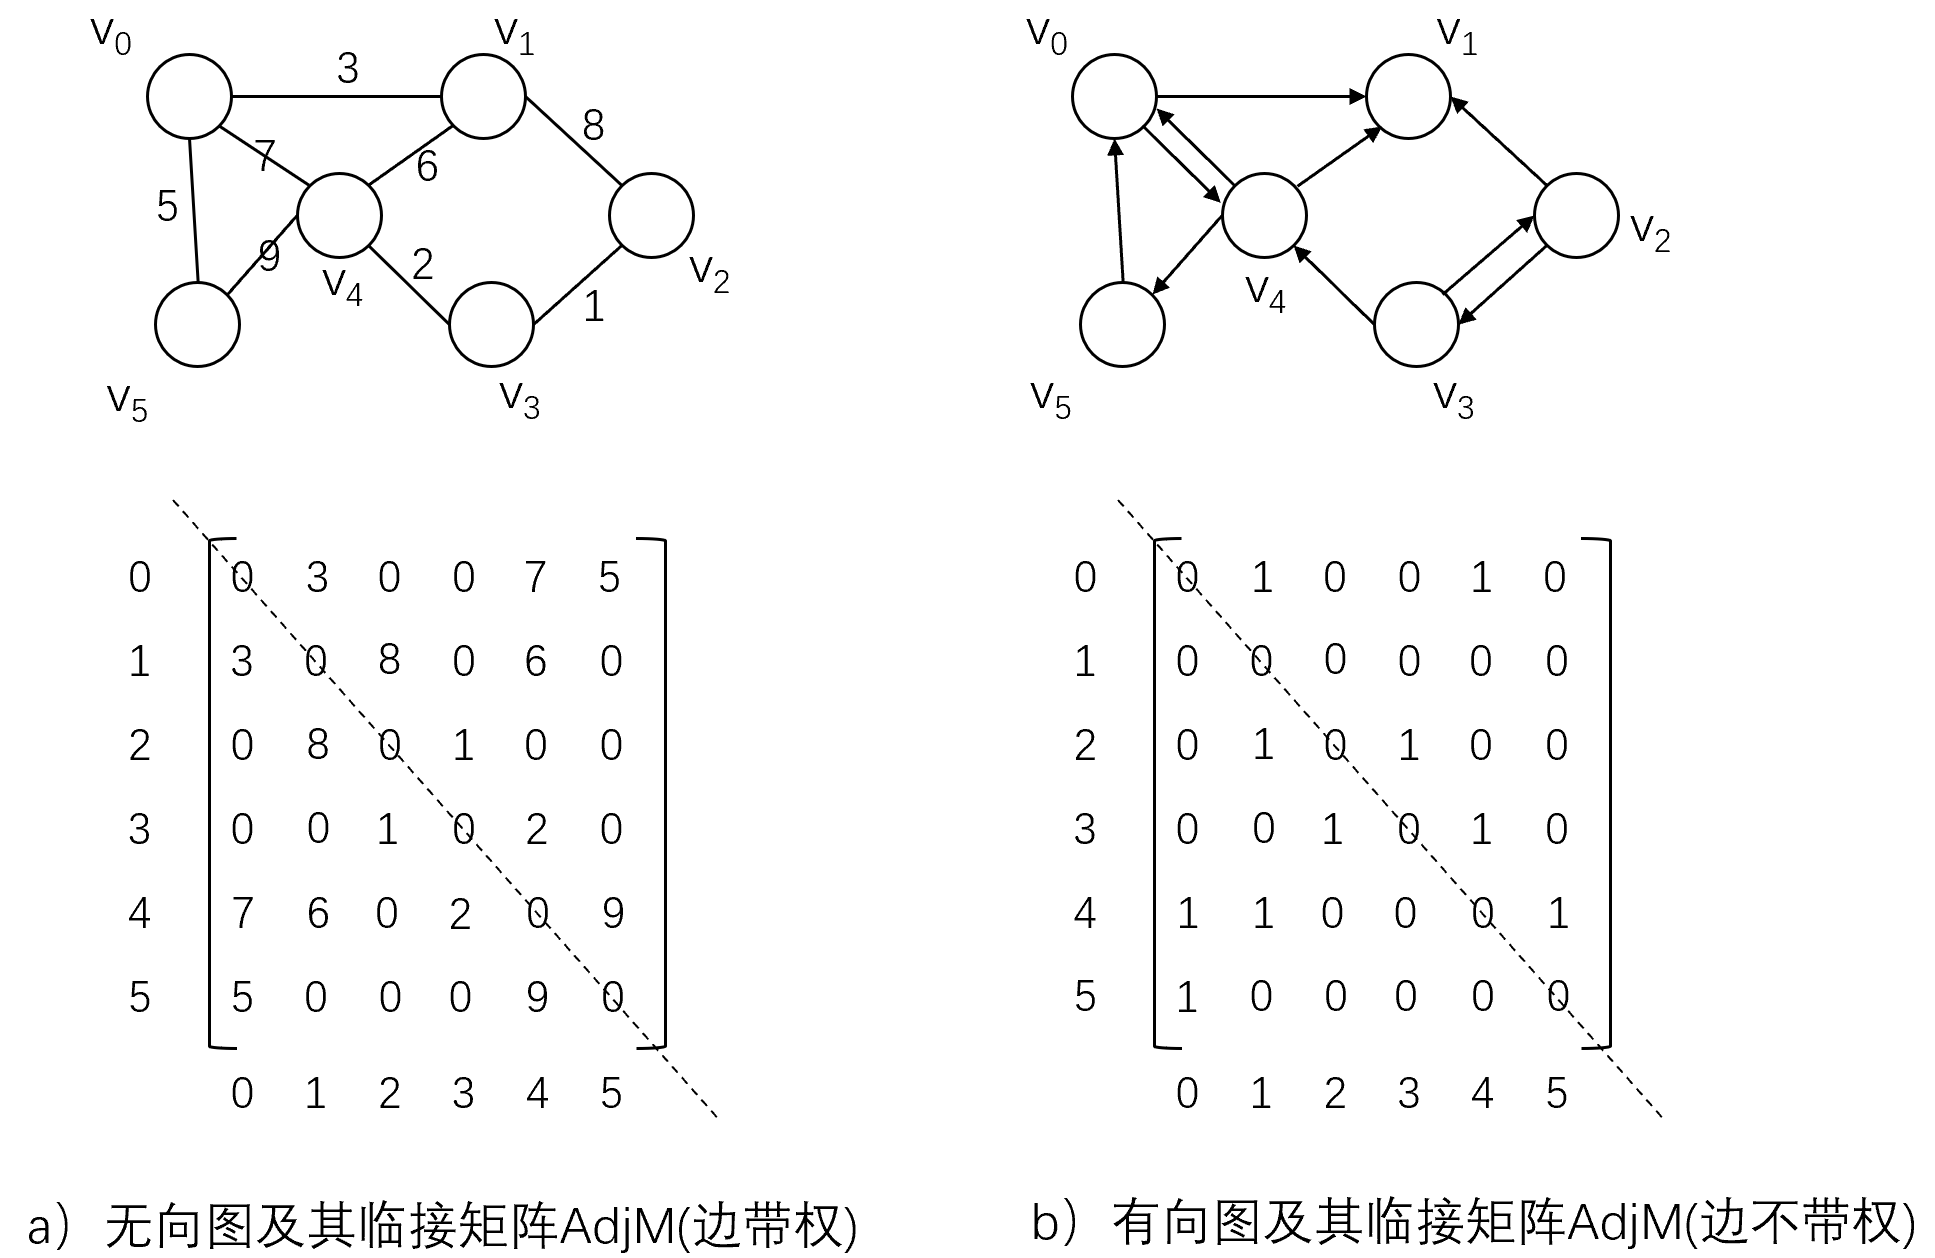
\includegraphics[width=0.93\textwidth]{assets/pics_and_ppts/ch5/邻接矩阵示意图.png}
    \caption{}
    \label{fig:邻接矩阵示意图}
\end{figure}
可以看出，a）是对称矩阵。

另一个指挥官\uline{麦丽凯}研究了格佛莱的提议后，对此法大为认同，但也指出了该方法的一个缺点：该方法存储图需要一个二维矩阵，存储具有N个顶点
的图，空间复杂度就是$O(N^2)$。若图存在大量顶点，这种方法在空间上难以接受。经过思考，麦丽凯提出了一种新的方法，后来被称为\term{邻接表}法。

\subsection{邻接表}
邻接矩阵的方法着眼于全局，直接从全局视角记录边与点的关系。而邻接表法则是将每一个顶点作为主角，记录每个顶点的“局部信息”。

具体来说，对于有N个顶点（编号为0, 1, ..., N-1）的图G，邻接表法会存储所有顶点的所有\term{出边}的信息。
如图\ref{fig:04邻接表记录顶点的出边信息}中，对于编号为2的顶点$v_2$，我们需要记录它的三条出边，就需要分别记录这三条边
的\uline{终点}是哪个顶点，以及\uline{边权}是多少。

\begin{figure}[htbp]
    \centering
    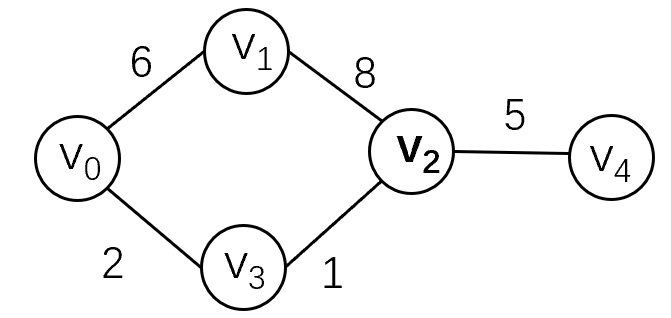
\includegraphics[width=0.33\textwidth]{assets/pics_and_ppts/ch5/04邻接表记录顶点的出边信息.png}
    \caption{}
    \label{fig:04邻接表记录顶点的出边信息}
\end{figure}
于是我们定义一个结构AdjEdge，来表示这种“出边”的信息：

\begin{cppcode}
    struct AdjEdge {
        int u;  // 邻接顶点的编号
        int weight; // 当前顶点到u的边的权值。若需要更多边的信息，可自定义EdgeInfo类型
    };
\end{cppcode}
由于无法确定每个顶点有多少条出边，因此，\bookmarkref{bookmark:waypoint-6}{waypoint-6}处介绍的不定长数组vector用在此处就非常合适。
对于$v_2$，我们就可以通过一个元素类型为AdjEdge的vector，将其所有出边的信息记录下来：
\begin{cppcode}
    vector<AdjEdge> AdjL_v2;  // 顶点v2的所有出边信息
\end{cppcode}
这个表就称为\uline{$v_2$的邻接表}。$v_2$的邻接表如图\ref{fig:05v2的邻接表}所示。
\begin{figure}[htbp]
    \centering
    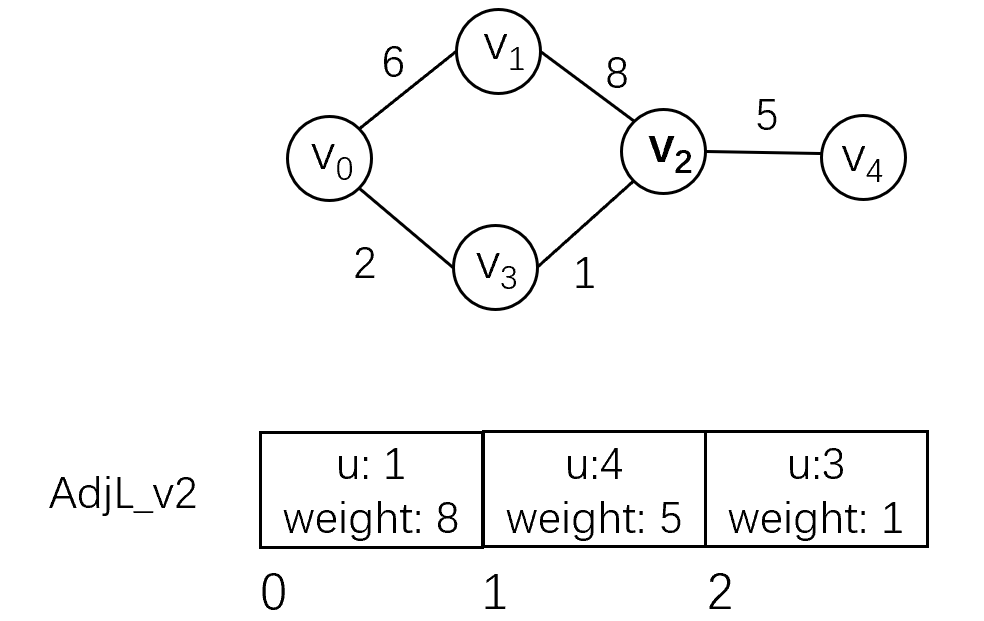
\includegraphics[width=0.48\textwidth]{assets/pics_and_ppts/ch5/05v2的邻接表.png}
    \caption{}
    \label{fig:05v2的邻接表}
\end{figure}

\begin{notebox}{提示}
    事实上很多时候，更好的做法是通过链表来实现邻接表（可以想想为什么），但二者思想是类似的。链表实现复杂，况且大多数情况下vector性能已经足够好。
    为了给大家带来更强的实用性，本章中邻接表拟采用vector实现。
\end{notebox}

某个顶点的邻接表记录了与该顶点有关的所有出边信息。
那么我们将图中所有顶点的出边信息都存储下来，也就是为每个顶点记录一个邻接表，一共记录N个邻接表，这也就完整地记录了图中所有边的关系：
\begin{cppcode}
    vector<AdjEdge> AdjList[N];  
\end{cppcode}
这N个顶点的邻接表共同构成了\uline{整个图G的邻接表}。注意：以上代码中AdjList是一个C原生数组，而AdjList[i]才是一个vector，该vector是顶点i的邻接表，保存
的是顶点i的所有出边的信息。

于是，使用邻接表存储图中边的信息，我们就可以将一个图表示为如下的结构：
\begin{cppcode}
    struct AdjEdge {
        int u;  // 邻接顶点的编号
        int weight; // 当前顶点到u的边的权值。若需要更多边的信息，可自定义EdgeInfo类型
    };
    struct LGraph {
        vector<AdjEdge> AdjList[MAX_VNUM];  // 邻接表
        VertexInfo v[MAX_VNUM];     // 存放顶点信息
        int current_vnum;           // 当前顶点数
        int current_enum;           // 当前边数
    };
\end{cppcode}

由于顶点v的邻接表记录的是顶点v的\term{出边}的信息，因此对于无向图，若存在边$(u,v)$，那么同时需要在AdjList[u] 中记录 v，并在 AdjList[v] 中记录 u。
因此，无向图中的一条实际边通常对应邻接表中的两个表项。

显然对于无权图，AdjEdge类型只存储邻接顶点的编号u即可。

前面的例子中的图及其完整的邻接表如图\ref{fig:06完整的邻接表示意}所示。
\begin{figure}[htbp]
    \centering
    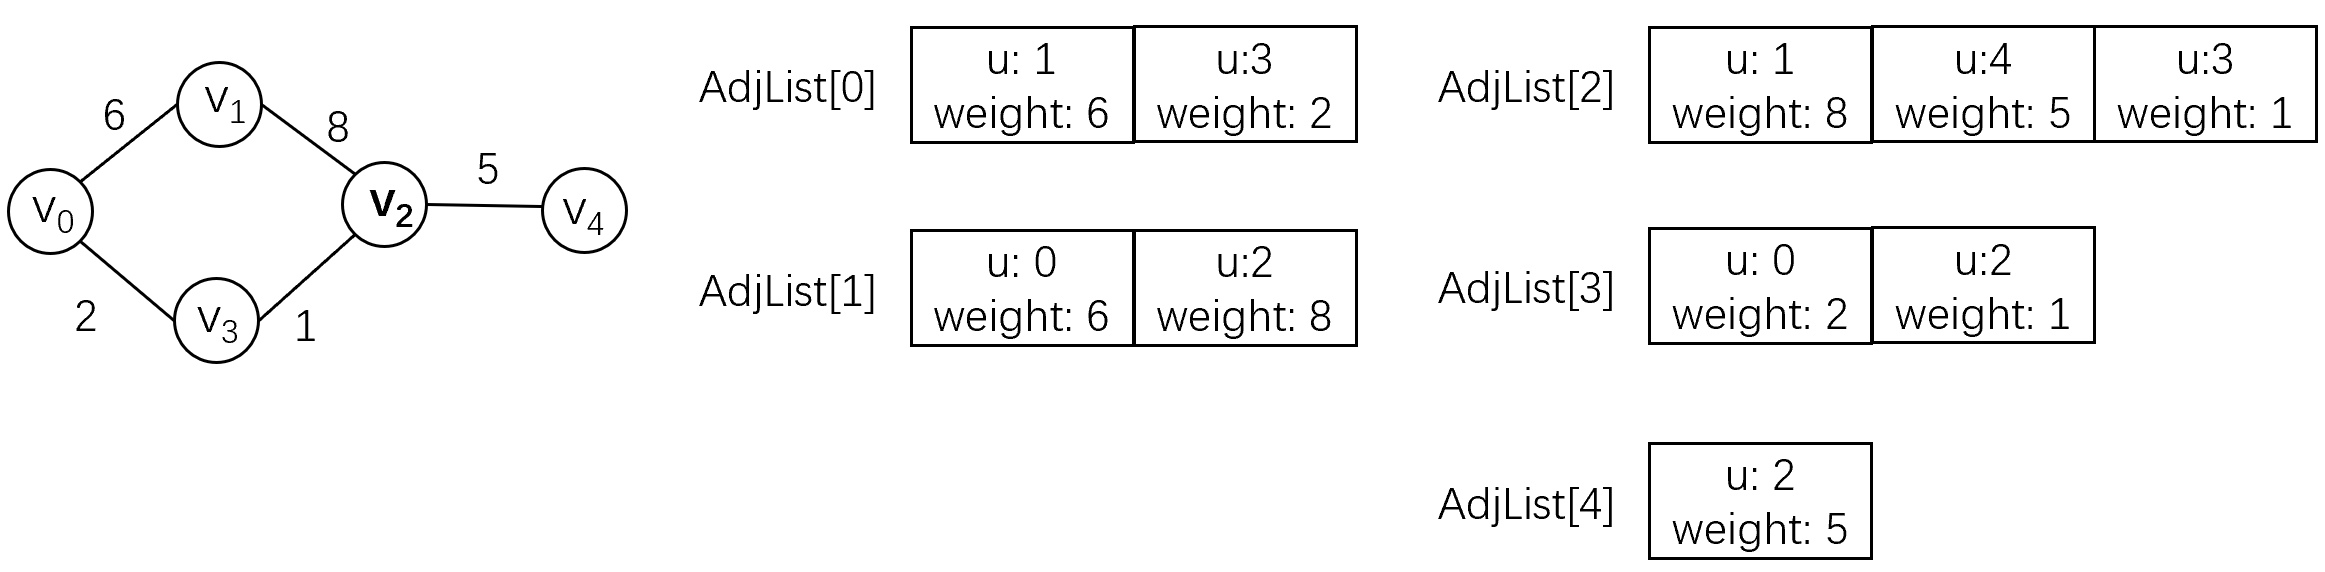
\includegraphics[width=1.02\textwidth]{assets/pics_and_ppts/ch5/06完整邻接表示意.png}
    \caption{}
    \label{fig:06完整的邻接表示意}
\end{figure}

容易知道邻接矩阵表示法下，存储一个图需要的存储空间与图的边数 $M$ 无关。而对于邻接表法，要存储有$N$个顶点、$M$条边的图，则需要维护$N$个邻接表，
对于无向图，总共需要$2M$个表项，对于有向图总共需要$M$个表项，因此，邻接表法存储一个图需要的存储空间为$O(N+M)$。\\

\subsection{二者获取邻接信息的对比}
可以看到，无论是邻接表存储法，还是邻接矩阵存储法，对于N个顶点的信息存储都是一致的，使用一个额外的数组来存储。二者区别就在于对于每个顶点的邻接信息，即
顶点与顶点、顶点与边的关系如何存储。二者存储方式的不同，也带来了一些获取邻接信息上的差异。

\noindent \Circled{1} 邻接矩阵

对于\uline{有向图}，要知道v的所有\uline{出边}信息，遍历一遍图的邻接矩阵的下标为v的那一行即可：
\begin{cppcode}
    for(int i=0; i<G.current_vnum; i++) {
        if(G.AdjM[v][i] != 0) {
            // v有一条到i的出边，G.AdjM[v][i]的值即是该边的权值
        } else {
            // v到i不存在出边
        }
    }
\end{cppcode}
类似地要知道v的所有入边信息，遍历下标为v的那一列即可。显然遍历的过程中若记录有效边的数量，就得到了顶点出度、入度的信息。

对于\uline{无向图}，只遍历下标为v的行或下标为v的列即可得到该顶点的所有邻接信息。
\begin{cppcode}
    for(int i=0; i<G.current_vnum, i++) {
        if(G.AdjM[v][i] != 0) {
            // v到i存在无向边，G.AdjM[v][i]的值即是该边的权值
        } else {
            // v到i不存在边
        }
    }
\end{cppcode}
同样地，若遍历过程中记录有效边的数量，就得到了无向图某顶点度的信息。

\noindent \Circled{2} 邻接表

对于邻接表存储的\uline{有向图}，v的邻接表存储的就是v的所有出边信息。要知道顶点v的所有\uline{出边信息}很简单，遍历v的邻接表即可：
\begin{cppcode}
    for(int i=0; i<G.AdjList[v].size(); i++) {
        // G.AdjList[v][i]就是v的邻接表的第i个表项，即与v邻接的第i个顶点和边权的信息。
    }
\end{cppcode}
同时，表长G.AdjList[v].size()就是顶点v的出度。

但是，对于邻接表存储的有向图，要知道顶点v的所有\uline{入边信息}，就需要将所有顶点的邻接表均查找一遍：
\begin{cppcode}
    // 遍历一遍所有顶点的邻接表
    for(int i=0; i<G.current_vnum; i++) {
        // 遍历顶点i的邻接表的所有表项
        for(int j=0; j<G.AdjList[i].size(); j++) {
            // 顶点i的第j个邻接点为v
            if(G.AdjList[i][j].u == v) {
                // 找到了v的一条入边，这是一条从i指向v的边，权值为G.AdjList[i][j].weight
                // 若需要计算v的入度，在此处累加。
            }
        }
    }
\end{cppcode}

二者对比如表\ref{table:邻接矩阵与邻接表的操作效率对比}所示：
\begin{table}[htbp]
    \centering
    \caption{邻接矩阵与邻接表的操作效率对比}
    \begin{tabular}{|l|c|c|}
        \hline
        操作 & 邻接矩阵 & 邻接表 \\
        \hline
        查找顶点 $v$ 的所有出边
        & $O(N)$
        & $O(\deg^+(v))$ \\
        \hline
        查找顶点 $v$ 的所有入边
        & $O(N)$
        & $O(N+M)$ \\
        \hline
        获取有向图顶点 $v$ 的出度
        & $O(N)$
        & $O(1)$（直接读取表项数量） \\
        \hline
        获取有向图顶点 $v$ 的入度
        & $O(N)$
        & $O(N+M)$（未额外维护入边信息） \\
        \hline
    \end{tabular}
    \label{table:邻接矩阵与邻接表的操作效率对比}
\end{table}
这里 \(N\) 表示顶点数，\(M\) 表示边数，\(\deg^+(v)\) 表示顶点 \(v\) 的出度。


有了以上扎实的模型基础，指挥官们计划了第一步行动。他们决定先从首都派出一名信使，将大敌来犯的消息通知到每一个据点的士兵以及居民们。
然而，各据点之间的道路错综复杂，信使不可能毫无章法地四处奔走。怎样规划通知顺序，才能确保每个据点都不会遗漏？

\section{图的遍历}

指挥官们给出了两种方式，也是王国的后来者总结出的两种图的遍历方式，总结如下。
\subsection{深度优先搜索（DFS）}
深度优先搜索（Depth First Search, DFS）的过程就像是“不分黑白地一股脑儿往前冲，直到撞了墙，才按原路返回，继续探索未探索过的其他路（当然也是继续冲、撞墙、返回，冲、撞墙、返回......）。”

具体来说，信使从首都（起点，记为v）出发，访问与v邻接且未被访问过的任意一个顶点u，
之后从u出发（而非回到v），再访问与u邻接且未被访问过的任意一个顶点u\textquotesingle，之后从u\textquotesingle 出发，继续访
问与u\textquotesingle 邻接且未被访问过的任意一个顶点u\textquotesingle \textquotesingle，......，如此重复，
直至不能继续访问下去之后，依次退回到最近被访问的顶点，若其还有未被访问的邻接顶点，则访问之......如此重复，直至图中所有顶点均被访问一遍。

我们以图\ref{fig:深度优先搜索过程}直观地感受一下深度优先搜索的过程。

假设起点为$v_0$：\\[0.3em]
a）访问$v_0$，然后看到与$v_0$邻接的顶点有$v_1$和$v_3$，他们都未被访问，任意选一个访问即可。假设选$v_1$。\\[0.3em]
b）访问$v_1$，然后看到邻接顶点仅有$v_2$未被访问，于是\\[0.3em]
c）访问$v_2$，看到$v_4$、$v_5$均未被访问，假设选$v_4$，于是\\[0.3em]
d）访问$v_4$，此时已深入最深处，与$v_4$邻接的所有顶点均已访问完成，于是退回到上一个顶点$v_2$，发现它还有$v_3$、$v_5$两个邻接顶点未访问，任选一个，
假设选$v_3$。\\[0.3em]

\begin{figure}[htbp]
    \centering
    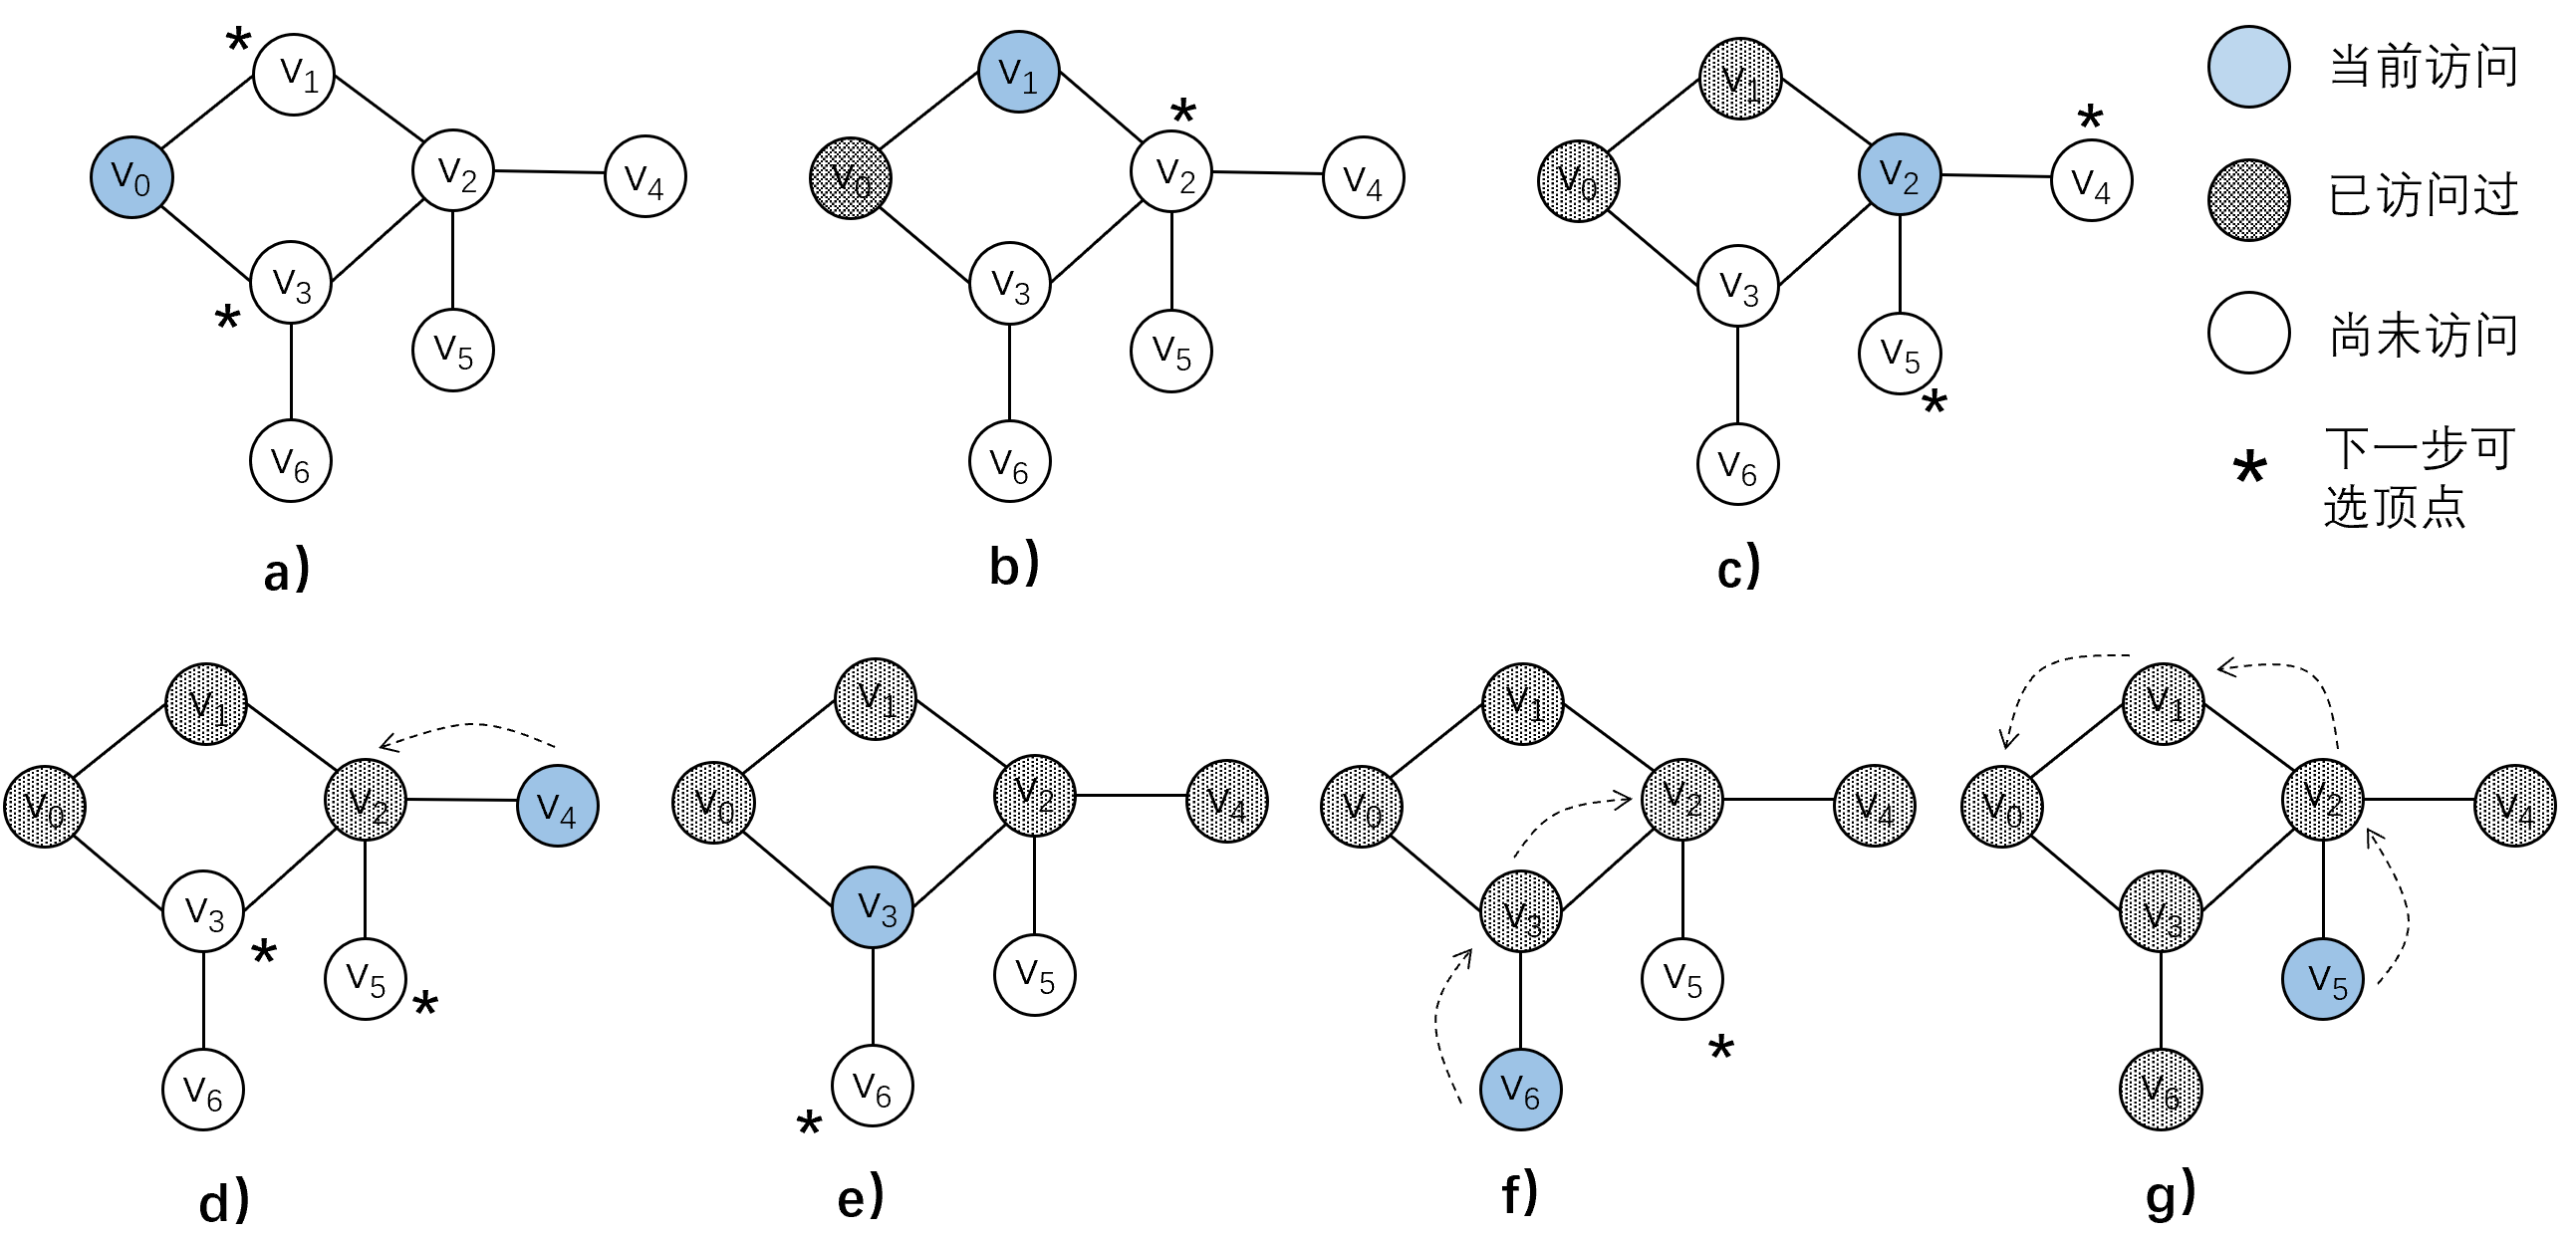
\includegraphics[width=1.08\textwidth]{assets/pics_and_ppts/ch5/07深度优先遍历过程.png}
    \caption{深度优先搜索}
    \label{fig:深度优先搜索过程}
\end{figure}

\noindent e）访问$v_3$，看到邻接的$v_6$还没被访问。于是\\[0.3em]
f）访问$v_6$，此时无法继续访问下去，于是退回到$v_3$，发现$v_3$的所有邻接顶点也都已经访问完成了，于是退回$v_2$，发现与$v_2$邻接的$v_5$还未访问。于是\\[0.3em]
g）访问$v_5$。之后退回到$v_2$（无顶点未访问），$v_1$（无顶点未访问）、$v_0$（无顶点未访问），深度优先搜索过程结束。

以上过程得到的深度优先访问序列为：\{$v_0$, $v_1$, $v_2$, $v_4$, $v_3$, $v_6$, $v_5$\}。
这就是深度优先搜索，总是尽可能“深”地探索，当无法再深入之后才原路返回，探索那些未走过的路。


\subsection{广度优先搜索（BFS）}
如果说深度优先搜索（DFS）是“一路走到底，不撞南墙不回头”，那么广度优先搜索（Breadth First Search, BFS）就是“浅尝辄止，先慢慢探清周围环境，再继续往深处走”。

实际上广度优先搜索和树的层序遍历非常相似。可以想象平静的水面落下一个小铁球而泛起层层涟漪，广度优先搜索即是先访问中心点，之后访问距中心点最近的“第一层涟漪”，
之后访问“第二层涟漪”，第三层......，直到全部访问完成。

具体来说，假设从v出发，首先访问起始顶点v，并“发现”v的所有未被访问的邻接顶点$v_1$, $v_2$, ..., $v_n$，这些顶点即是“第二层涟漪”，依次访问它们，访问时，
又会发现第三层涟漪$v_{11}$, $v_{12}$, ..., $v_{nm}$......如此往复，直至图中所有顶点均被访问一遍。\\

我们以图\ref{fig:广度优先遍历过程}来直观地感受一下广度优先搜索的过程。拟以$v_0$作为起点：\\[0.3em]
a）访问$v_0$，看到$v_0$的邻接顶点有$v_1$和$v_3$，于是将这两个顶点作为“第二层”的顶点，此时“第一层涟漪”已访问完毕，“第二层涟漪”有两个，任选一个，假设
选择$v_1$；\\[0.3em]
b）访问$v_1$，此时发现了“第三层涟漪”的一个顶点$v_2$，先将它记下来。准备继续访问第二层未访问完的顶点$v_3$。\\[0.3em]
c）访问$v_3$，发现$v_3$的邻接顶点$v_6$尚未被访问，因此也将它记下来，作为“第三层涟漪”的一部分。至此，第二层顶点均已访问完毕，准备访问第三层，假设选择
$v_2$；\\[0.3em]

\begin{figure}[htbp]
    \centering
    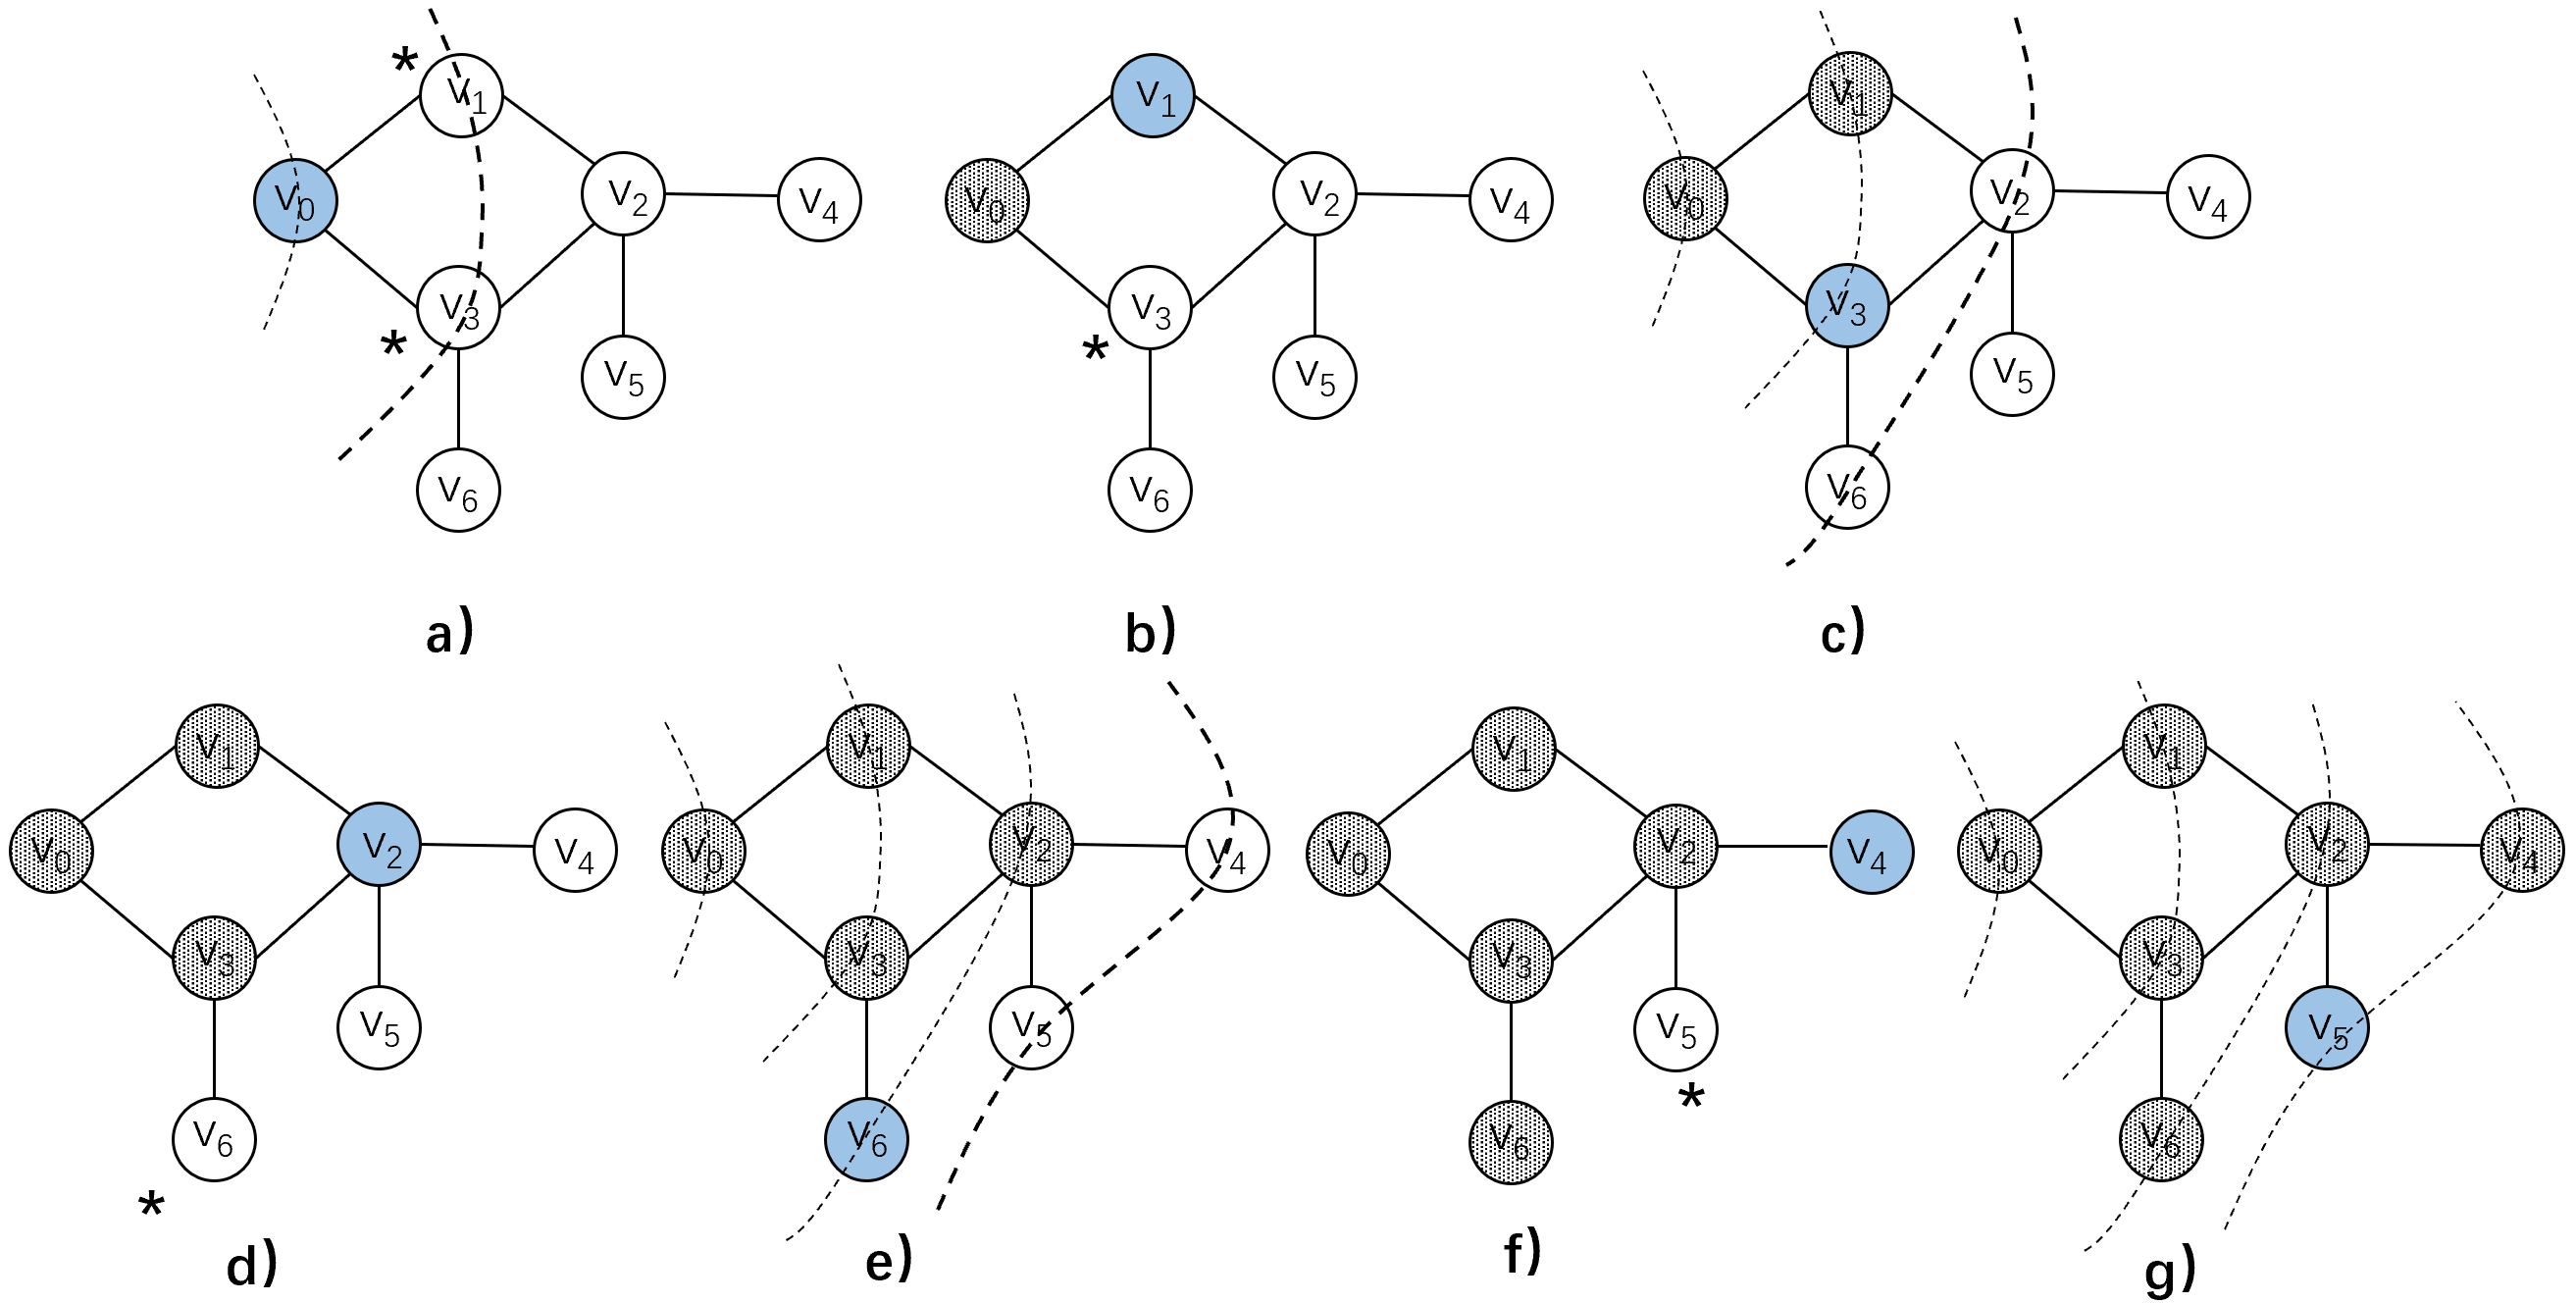
\includegraphics[width=1.10\textwidth]{assets/pics_and_ppts/ch5/08广度优先遍历过程.png}
    \caption{广度优先搜索}
    \label{fig:广度优先遍历过程}
\end{figure}

\noindent d）访问$v_2$，发现与$v_2$邻接的有$v_4$和$v_5$还未访问，因此将它们记下来，作为“第四层涟漪”的一部分；然后准备访问第三层剩下的$v_6$；\\[0.3em]
e）访问$v_6$，$v_6$没有尚未访问的邻接顶点，因此从$v_6$没有发现新的“第四层涟漪”。至此第三层均已访问完毕。准备开始访问第四层\\[0.3em]
f）访问$v_4$，没发现新的顶点；\\[0.3em]
g）访问$v_5$，没发现新的顶点。此时所有顶点均已访问过一遍，没有新的层了，结束。\\[0.3em]

以上过程得到的广度优先搜索访问序列是\{$v_0$, $v_1$, $v_3$, $v_2$, $v_6$, $v_4$, $v_5$\}。这就是广度优先搜索，总是先“摸清楚周围
的环境，再继续向更深处进发”。BFS算法可以求解无权图或等权图的最短路径问题，我们将在{\color{red}习题6第16、17题}中详细介绍。

至此，“深”和“广”的语义已经很明确，“深度优先”总是冲到最“深”处，而“广度优先”总是先向“广”阔的四周探索。




\subsection{DFS和BFS的实现}
可以看到，广度优先搜索（BFS）总是“越早看见的顶点越先被访问”（因为层数小），而深度优先搜索（DFS）总是“越晚看见的顶点越先被访问”（因为一路往前冲而不是回头）。
这正与队列和栈的“先进先出”与“后进先出”的特点相符合。

如果你研究过\bookmarkref{bookmark:waypoint-3}{waypoint-3}处的问题，可以
进一步理解：实际上广度优先（BFS）的过程中，“顶点们”成为了“仍然等待某事发生，并且优先处理\uline{先来者}的数据”，而深度优先（DFS）的过程中，“顶点们”则是“仍然
等待某事发生，并且优先处理\uline{后来者}的数据”：
\begin{enumerate}
    \item 在广度优先（BFS）中，顶点们等待被访问，并且先“被看见”的先访问；
    \item 而在深度优先（DFS）中，顶点们等待被访问，并且后“被看见”的先访问。
\end{enumerate}

有了以上思维过程，我们就可以非常清晰地给出二者的代码实现过程。

\minisection{深度优先搜索（DFS）的实现}
创建一个栈s，访问起点，并将起点的所有邻接且尚未被访问过的顶点入栈。之后：
\begin{enumerate}
    \item 若栈空，说明没有待访问的顶点了，算法结束，否则，进入第二步；
    \item 从栈顶取出一个顶点，访问之，并将该顶点的所有邻接且未被访问过的顶点入栈；回到第一步。
\end{enumerate}
如此循环直至栈空，则所有顶点均被访问一遍。

如何确定某顶点是否已经访问过？最常见的办法是维护一个一维数组：
\begin{cppcode}
    bool visited[MAX_VNUM]; // 所有元素初始为false，表示还未访问
\end{cppcode}
visited[i]为true则表示已经访问过了。

以\uline{邻接矩阵}存储的图为例，深度优先搜索的代码如下所示：
\begin{cppcode}
/************** 邻接矩阵结构定义 ***************/
// // MAX_VNUM为该结构可存储的图的最大顶点数
//     struct MGraph { 
//         VertexInfo v[MAX_VNUM] ;
//         int AdjM[MAX_VNUM][MAX_VNUM];
//         int current_vnum;   // 当前顶点数
//         int current_enum;   // 当前边数
//     };

// 输入图G以及起点编号start_idx，以DFS方式对每一个顶点执行某函数visit()
void DFS(MGraph G, int start_idx) {
    bool visited[G.current_vnum];
    // 初始化visited[]数组
    for(int i=0; i<G.current_vnum; i++) {
        visited[i] = 0;
    }

    stack<int> s;   // 栈中存储顶点编号即可
    s.push(start_idx);
    visited[start_idx] = true;
    while(!s.empty()) {
        // 访问栈顶顶点v
        int v = s.top();
        s.pop();
        visit(G.v[v]);   // 访问v
        
        // 将与v邻接的所有尚未访问的顶点入栈
        for(int i=0; i<G.current_vnum; i++) {
            if(G.AdjM[v][i] != 0 && visited[i] == false) {
                s.push(i);
                visited[i] = true;
            }
        }
    } // end while
}
\end{cppcode}


若图是通过\uline{邻接表}存储的，与邻接矩阵存储的代码有什么区别呢？其实仅在寻找v的所有邻接点时，代码有区别。邻接表版本代码如下：
\begin{cppcodeHighlight}[14,31-37]
/************ 邻接表结构定义 *************/
// struct AdjEdge {
//     int u;  // 邻接顶点的编号
//     int weight; // 当前顶点到u的边的权值。
// };
// struct LGraph {
//     vector<AdjEdge> AdjList[MAX_VNUM];  // 邻接表
//     VertexInfo v[MAX_VNUM];     // 存放顶点信息
//     int current_vnum;           // 当前顶点数
//     int current_enum;           // 当前边数
// };

// 输入图G以及起点编号start_idx，以DFS方式对每一个顶点执行某函数visit()
    void DFS(LGraph G, int start_idx) {
        bool visited[G.current_vnum];
        // 初始化visited[]数组
        for(int i=0; i<G.current_vnum; i++) {
            visited[i] = 0;
        }

        stack<int> s;   // 栈中存储顶点编号即可
        s.push(start_idx);
        visited[start_idx] = true;
        while(!s.empty()) {
            // 访问栈顶顶点v
            int v = s.top();
            s.pop();
            visit(G.v[v]);   // 访问v
            
            // 将与v邻接的所有尚未访问的顶点入栈
            for(int i=0; i<G.AdjList[v].size(); i++) {
                // G.AdjList[v]是v的邻接表，G.AdjList[v][i]是该表中第i个元素
                int u = G.AdjList[v][i].u;
                if(visited[u] == false) {
                    s.push(u);
                    visited[u] = true;
                }
            }
        } // end while
    
    }
\end{cppcodeHighlight}

\minisection{广度优先搜索（BFS）的实现}
根据前面的思维过程很容易知道，将深度优先搜索代码中的栈换成队列即是广度优先搜索。邻接矩阵版：

\begin{cppcodeHighlight}[9-10,12-15,21]
// 输入图G以及起点编号start_idx，以BFS方式对每一个顶点执行某函数visit()
    void BFS(MGraph G, int start_idx) {
        bool visited[G.current_vnum];
        // 初始化visited[]数组
        for(int i=0; i<G.current_vnum; i++) {
            visited[i] = 0;
        }

        queue<int> q;   // 队列中存储顶点编号即可
        q.push(start_idx);
        visited[start_idx] = true;
        while(!q.empty()) {
            // 访问队首顶点v
            int v = q.front();
            q.pop();
            visit(G.v[v]);   // 访问v
            
            // 将与v邻接的所有尚未访问的顶点入队
            for(int i=0; i<G.current_vnum; i++) {
                if(G.AdjM[v][i] != 0 && visited[i] == false) {
                    q.push(i);
                    visited[i] = true;
                }
            }
        } // end while
    }
\end{cppcodeHighlight}

邻接表版：
\begin{cppcodeHighlight}[9-10,12-15,23]
// 输入图G以及起点编号start_idx，以BFS方式对每一个顶点执行某函数visit()
    void BFS(LGraph G, int start_idx) {
        bool visited[G.current_vnum];
        // 初始化visited[]数组
        for(int i=0; i<G.current_vnum; i++) {
            visited[i] = 0;
        }

        queue<int> q;   // 队列中存储顶点编号即可
        q.push(start_idx);
        visited[start_idx] = true;
        while(!q.empty()) {
            // 访问队首顶点v
            int v = q.front();
            q.pop();
            visit(G.v[v]);   // 访问v
            
            // 将与v邻接的所有尚未访问的顶点入队
            for(int i=0; i<G.AdjList[v].size(); i++) {
                // G.AdjList[v]是v的邻接表，G.AdjList[v][i]是该表中第i个元素
                int u = G.AdjList[v][i].u;
                if(visited[u] == false) {
                    q.push(u);
                    visited[u] = true;
                }
            }
        } // end while
    }
\end{cppcodeHighlight}
上面代码中使用到的stack和queue是C++标准库为我们提供的栈和队列的数据结构。我们曾在\bookmarkref{bookmark:waypoint-7}{waypoint-7}处介绍过。

\begin{thinkbox}
    你也许会有疑问，将visited[i]标记为true的时机，难道不应该是访问i之后吗？代码中怎么将i入队（还未访问）时就将visited[i]标记为true了？\\

    访问后标记当然是正确的做法。但事实上，入队时即标记同样是正确的，并且是更优的做法。你可以想一想，为什么正确？为什么更优？
    （可以结合图\ref{fig:广度优先遍历过程}的搜索过程思考）。
\end{thinkbox}

\vspace{\baselineskip}

以上便是图最常见的两种遍历方式：广度优先搜索和深度优先搜索。信使任选一种方式，即可确保每个据点都不会遗漏。但是，信使很快发现了这样一个问题，如图
\ref{fig:一个非连通图}所示，信使走到据点A后，发现通往D、E的桥梁已经倒塌，而他无论如何也找不到其他路通往D、E这两个城镇。

\begin{wrapfigure}{r}{0.38\textwidth}
    \centering
    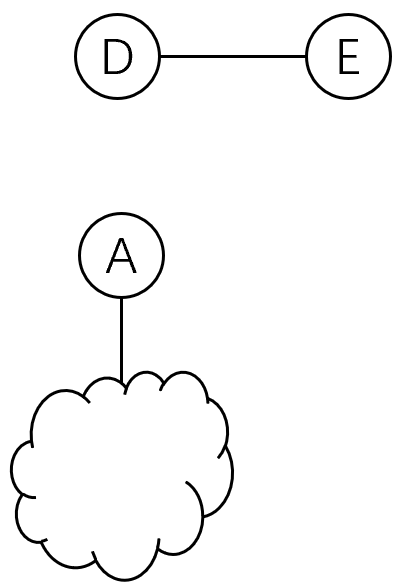
\includegraphics[width=0.19\textwidth]{assets/pics_and_ppts/ch5/09一个非连通图.png}
    \caption{无法抵达对岸的城镇}
    \label{fig:一个非连通图}
\end{wrapfigure}

信使回去汇报后，指挥官们发现类似的\textbf{非连通}区域还有很多，于是立即快马加鞭地组织人手修路搭桥，将王国地图修复成了一个\term{连通图}。

思渡者啊，你也许会想，若实际中某图存在从起点出发不可达的顶点，即图是一个非连通图，该如何遍历它呢？其实只需要对图中每一个顶点均执行一次上面的DFS或BFS即可，
以图\ref{fig:一个非连通图}为例，伪代码如下：

\begin{cppcode}
    Graph G;    // 假设G已经存储了图@\ref{fig:一个非连通图}@所示的图
    for(int i=0; i<N; i++) {
        if(!visited[i]) {
            DFS(G, i);
        }
    }
\end{cppcode}
以上代码会对G中所有顶点（包括顶点D、E、A等）依次判断，若未访问过，则对其执行DFS。显然，当首次对A所在的连通块执行DFS时，会将其中所有顶点标记为已访问，之后
循环中判断时，则不会对连通块中的其他顶点执行DFS了。D和E所在的连通块有类似的情况。\\

以上两种遍历的实现都是非递归实现。事实上，由于深度优先搜索的特性，通过递归的方式实现深度优先搜索是非常简单的：
\begin{cppcode}
    bool visited[N];    // 初始化为false
    void DFS(int v) {
        visit(v);   // 访问v
        visited[v] = true;
        // 递归地访问v的邻接点，适配邻接矩阵或邻接表就行了。
        for(v的每一个邻接点u) { 
            if(!visited[u]) {
                DFS(u);
            }
        }
    }
\end{cppcode}
要遍历非连通图，分别以每一个顶点为起点调用以上函数即可：
\begin{cppcode}
    void Travel() {
        for(int i=0; i<N; i++) {
            DFS(i);
        }
    }
\end{cppcode}
由于递归调用过程中，操作系统要开出很多个函数栈，因此递归的方式往往空间复杂度更大，但递归算法在很多情况下也是有用的。\\


根据指挥官给出的方法，信使无一疏漏地将大敌来犯的消息传遍了王国的每一座城池、每一座要塞。士兵和居民们纷纷武装起来，布起防御系统，准备迎接那场即将到来的大战。

\chapter*{--- BONFIRE ENCOUNTERED ---}%%%%%%%%%%%%%%%%%%%%%%%%%%%%%%%%%%%%%%%%%%%%%%%%%%%%%%%%%%%%%%%%%%%%%%%%%%%%%%%%%%%%%%%%%%%%%%%%%%%%%%%%%%%%%%%%%%%%%%%%%%%%%%%%%%%%%%%%%%
\begin{exercise}
1. 关于下图所示的无向图，下列说法错误的是\underline{\hspace{1cm}}
\begin{center}
    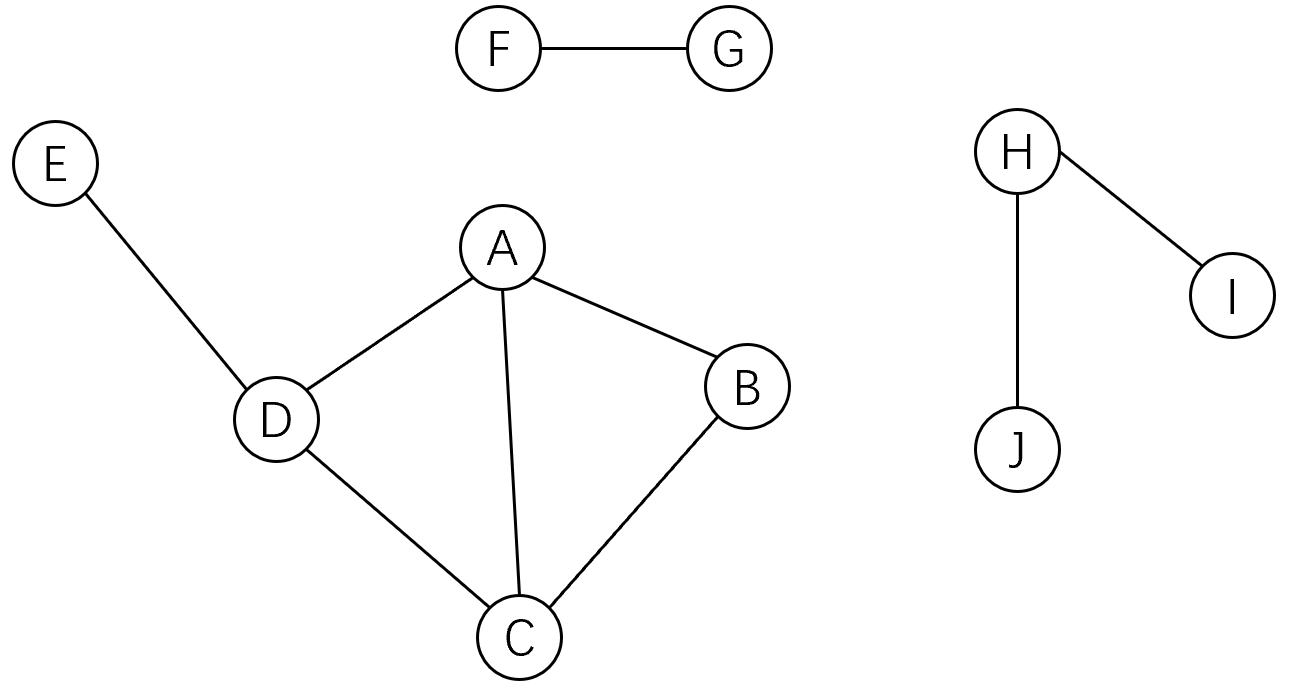
\includegraphics[width=0.48\textwidth]{assets/pics_and_ppts/ch5/习题01，图的基本概念.png}
\end{center}

\noindent A. 顶点A的度为3\\
B. 顶点A与顶点E是不连通的\\
C. 该图有3个连通分量\\
D. 对于顶点H所在的连通分量，若以H为起点，其深度优先搜索序列可以是\{H, I, J\}\\

2. 关于下图所示的有向图$G$以及其三个子图$G_1$, $G_2$, $G_3$，下列说法错误的是\underline{\hspace{1cm}}

\begin{center}
    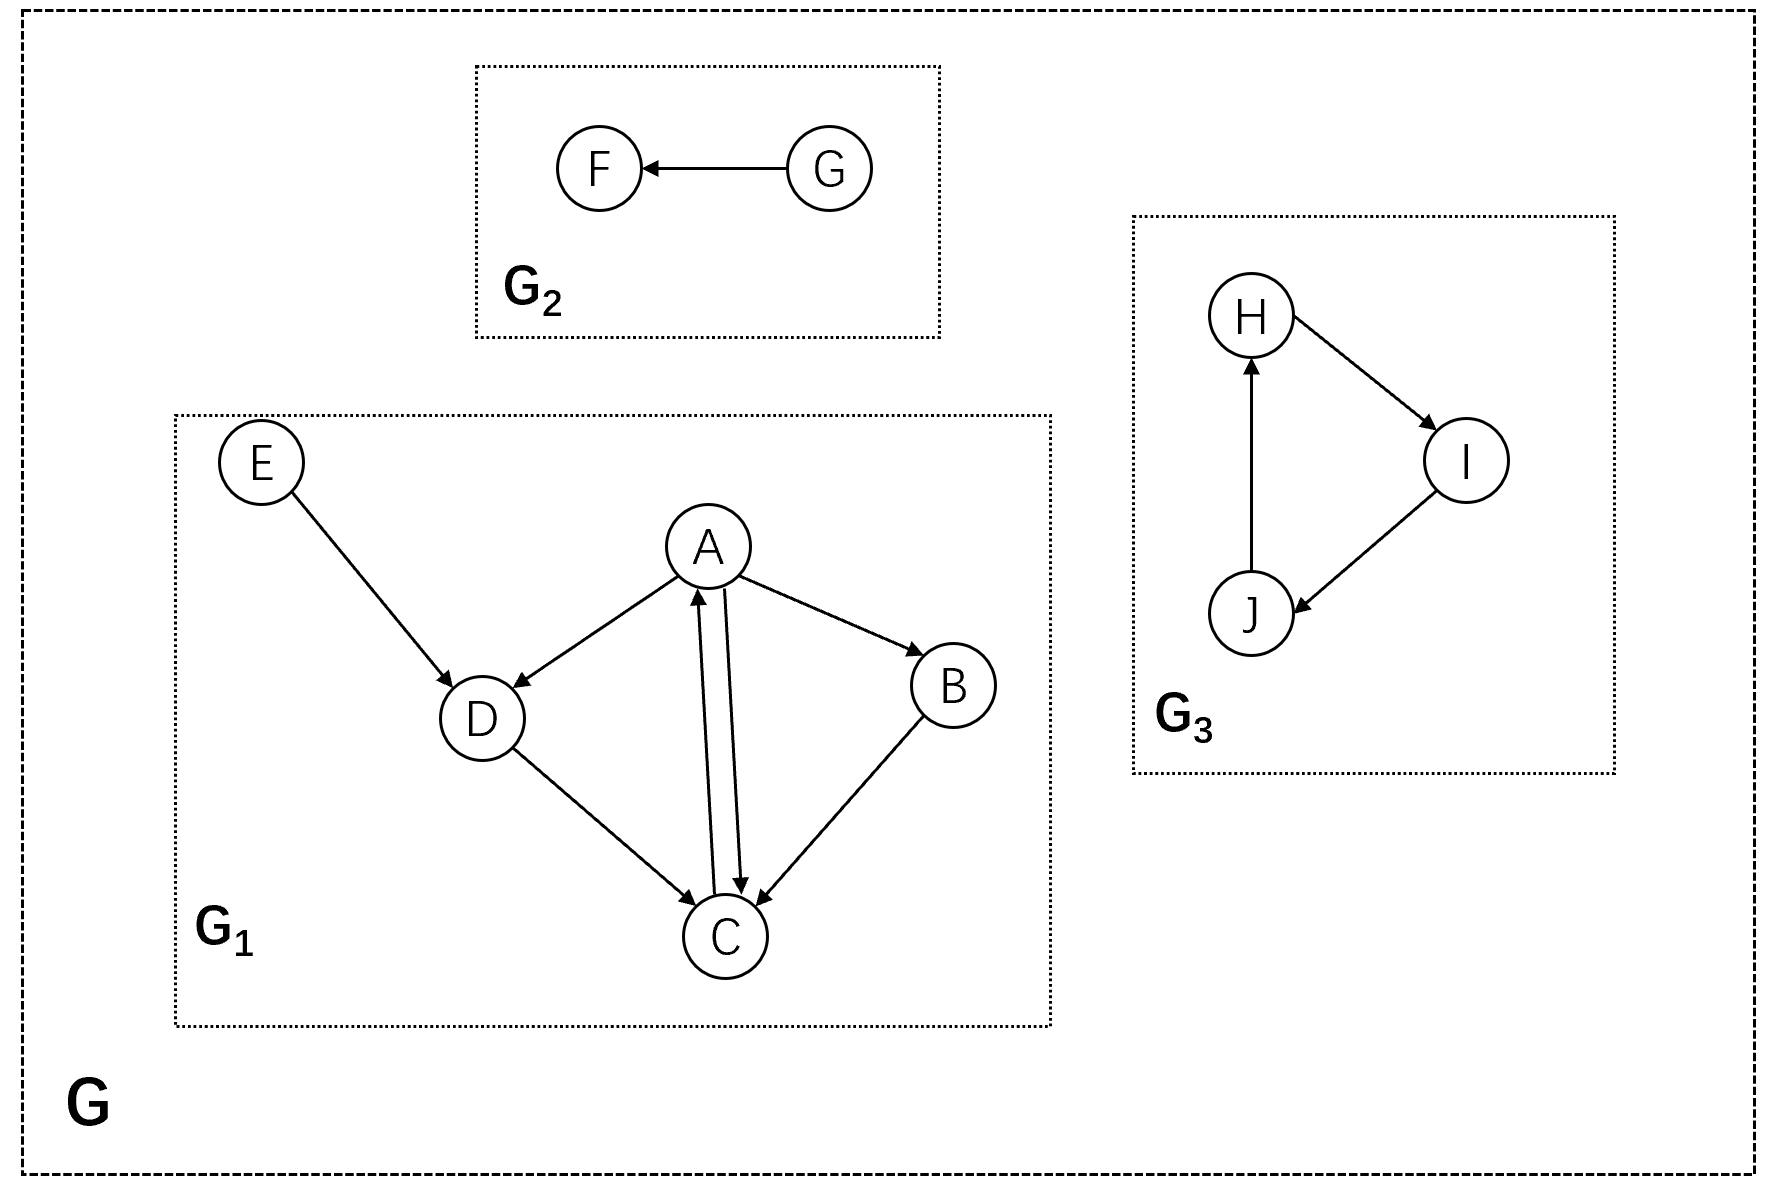
\includegraphics[width=0.72\textwidth]{assets/pics_and_ppts/ch5/习题02，图的基本概念.png}
\end{center}

\noindent A. 三个子图$G_1$, $G_2$, $G_3$中，仅$G_3$是强连通的\\
B. 图G的强连通分量数大于3\\
C. 顶点A的出度为3\\
D. 顶点F的出度为1\\

3. （某年408真题）下列关于无向连通图特性的叙述中，正确的是\underline{\hspace{1cm}}。

\(\mathrm{I}\). 所有顶点的度之和为偶数。

\(\mathrm{II}\). 边数大于顶点个数减 1。

\(\mathrm{III}\). 至少有一个顶点的度为 1。\\
A. 只有 \(\mathrm{I}\) \\
B. 只有 \(\mathrm{II}\) \\
C. \(\mathrm{I}\) 和 \(\mathrm{II}\) \\
D. \(\mathrm{I}\) 和 \(\mathrm{III}\) \\

4. 思考：有N个顶点的无向图，至多有多少条边？（不允许存在自环和重复边）。\\

5. 思考：有N个顶点的无向图，要保证它是连通图，至少要有多少条边？\\

6. （某年408真题）若无向图$G=(V, E)$有7个顶点，无边。现在要向图$G$中添加若干条边。请问，要保证无论怎样添加，添加$N$条边后图一定是连通的，则$N$最小是\underline{\hspace{1cm}}\\[0.5em]
\begin{tabular}{llll}
    A. 6 & B. 15 & C. 16 & D. 21
\end{tabular}

\vspace{\baselineskip}

7. 设某无向图的邻接矩阵A如下所示，若0表示边不存在，则各顶点的度依次是\underline{\hspace{1cm}}\\
\[
A =
\begin{bmatrix}
0 & 1 & 0 & 1 \\
1 & 0 & 1 & 1 \\
0 & 1 & 0 & 0 \\
1 & 1 & 0 & 0
\end{bmatrix}
\]

\begin{tabular}{llll}
    A. 2,3,1,2 & B. 4,6,2,4 & C. 0,1,2,3 & D. 999,1000,1001,7820
\end{tabular}

\vspace{\baselineskip}

8. 若上题的矩阵A表示的是某有向图的邻接矩阵，则各顶点的度依次是\underline{\hspace{1cm}}

提示：有向图中顶点的度定义为该顶点的入度和出度之和。\\[0.5em]
\begin{tabular}{llll}
    A. 2,3,1,2 & B. 4,6,2,4 & C. 0,1,2,3 & D. 999,1000,1001,7820
\end{tabular}

\vspace{\baselineskip}

9. 如下图所示的图$G$若使用邻接表存储，顶点A和C的邻接表表长分别是多少？\underline{\hspace{1cm}}\\

\begin{center}
    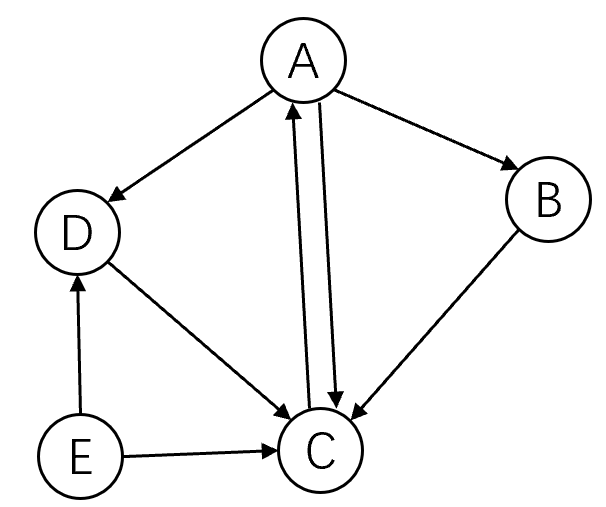
\includegraphics[width=0.27\textwidth]{assets/pics_and_ppts/ch5/习题05，邻接表表长.png}
\end{center}

\begin{tabular}{llll}
    A. 3,3 & B. 1,4 & C. 3,1 & D. 4,4
\end{tabular}

\vspace{\baselineskip}

10. 对于上题图以顶点E为起点进行深度优先搜索，不可能得到的搜索序列是\underline{\hspace{1cm}}\\
\begin{tabular}{ll}
    A. \{E,D,C,A,B\}& B. \{E,C,A,D,B\}\\
    C. \{E,C,A,B,D\}& D. \{E,C,D,A,B\}\\
\end{tabular}

\vspace{\baselineskip}

11. 对于下图所示的图$G$，以0号顶点为起点进行广度优先搜索，不可能得到的序列是\underline{\hspace{1cm}}\\
\begin{center}
    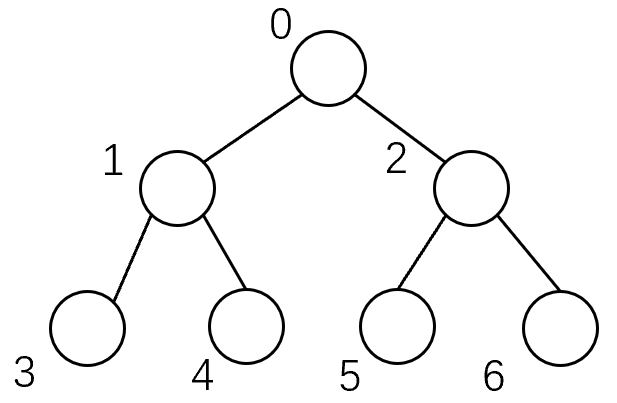
\includegraphics[width=0.33\textwidth]{assets/pics_and_ppts/ch5/习题06，树上的广度优先.png}
\end{center}
\begin{tabular}{ll}
    A. \{0,1,2,3,4,5,6\}& B. \{0,2,1,6,5,4,3\}\\
    C. \{0,3,4,5,6,1,2\}& D. \{0,1,2,3,4,6,5\}\\
\end{tabular}

\vspace{\baselineskip}

12. 关于图的两种遍历算法：深度优先搜索（DFS）和广度优先搜索（BFS），下列说法错误的是\underline{\hspace{1cm}}\\[0.5em]
A. 深度优先搜索通常通过队列实现，而广度优先搜索通常通过栈实现\\
B. 对于同一个图，深度优先搜索、广度优先搜索序列可能不唯一，取决于具体实现\\
C. 深度优先搜索能够访问到起点所在连通块的每一个顶点，不会遗漏 \\
D. 广度优先搜索能够访问到起点所在连通块的每一个顶点，不会遗漏\\

13. 对于有N个顶点，未知边数的无向无权图$G$, 分别编写以下两个函数：\\[0.5em]
1）若图G采用邻接矩阵存储，求其所有顶点的度数之和：
\begin{cppcode}
    bool AdjM[N][N];    // 假设该数组已经正确存储了G的邻接矩阵
    // 返回所有顶点的度数之和
    int DegreeSum(int N) {
        // 在此处完成你的代码
    }
    
\end{cppcode}

2）若图G采用邻接表存储，求其所有顶点的度数之和；
\begin{cppcode}
    vector<int> AdjList[N]; // 该数组已经正确存储了G的邻接表
    // 返回所有顶点的度数之和
    int DegreeSum(int N) {
        // 在此处完成你的代码
    }
\end{cppcode}

随意画出一个无向图，脑中模拟你代码的运行过程并计算出结果，你发现了什么规律吗？对于有向图有类似的规律吗？\\\\



【14、15、16、17、18题基于此背景】传说在《前有数据结构》大陆某处神秘的角落有一片森林，其中有一棵樱花树无时不刻地施展着她的魔法，为世人祈福，带来幸运。可是
该魔法也无时不刻地侵蚀着她自身，这些痛苦会凝聚成泪滴积于花瓣之上，将其饮下，便能抚平樱树的悲怆，化作自身的庇佑。

火光摇曳中，你在帐篷中沉睡过去。维火女凝视着你满身的疲惫与疮痍，眼底盛满了心疼与依恋。她不再忍心见你独自背负这苦难，便悄然别过营火，
孤身涉足那片未知的森林，去寻找并带回那代表着祝福与庇佑的樱花之泪。

天亮了。维火女已到达了那片森林。你通过火焰之环看到了那片森林的地图。森林中有N(N<=100)棵树木，编号为0到N-1，一些树木之间通过双向的灵魂通路相连，
而有些树木则无法抵达。\\


14. 维火女从编号为0的树木处出发，试图探索可达的所有树木，以找到那具有魔法的樱花树。假设地图采用邻接表存储，请你编写一个递归版本的DFS函数，计算维火女从起点0出发，
总共可以访问到的可达树木有多少棵？（包含起点本身）。

\begin{cppcode}
    const int N/* = 100*/;
    bool visited[N];    // 已初始化为false

    // AdjList[i] 已存放编号为i的顶点的邻接表，邻接表元素类型int，含义为与i邻接的顶点编号
    int CountAccessibleTrees(vector<int> AdjList[N]) {
        
    }
\end{cppcode}

\vspace{\baselineskip}

15. 假设地图采用邻接表存储，请你用非递归的DFS或BFS计算，这片森林有多少个连通块？
\begin{cppcode}
    const int N/* = 100*/;
    bool visited[N];    // 已初始化为false

    // AdjList[i] 已存放编号为i的顶点的邻接表，邻接表元素类型int，含义为与i邻接的顶点编号
    int CountConnectedComponents(vector<int> AdjList[N]) {
        
    }
\end{cppcode}

\vspace{\baselineskip}

*16. N棵树木的信息已存储于一个char类型的数组中：
\begin{cppcode}
    char trees[N];
\end{cppcode}
若某棵树是普通树木，其值为\textquotesingle F\textquotesingle, 若它是那棵魔法樱树，则其值为\textquotesingle T\textquotesingle。
假设地图采用\term{邻接矩阵}存储，维火女从起点u出发，能否抵达樱花树？若能，输出一条可行的路径，否则输出“......”。

以下图地图为例，若起点u为0，你可以输出“01356”、“0356”或“0231456”等，但不能输出“0456”、“06”等等不合法的路径；若起点u不在此连通块，输出“......”。
\begin{center}
    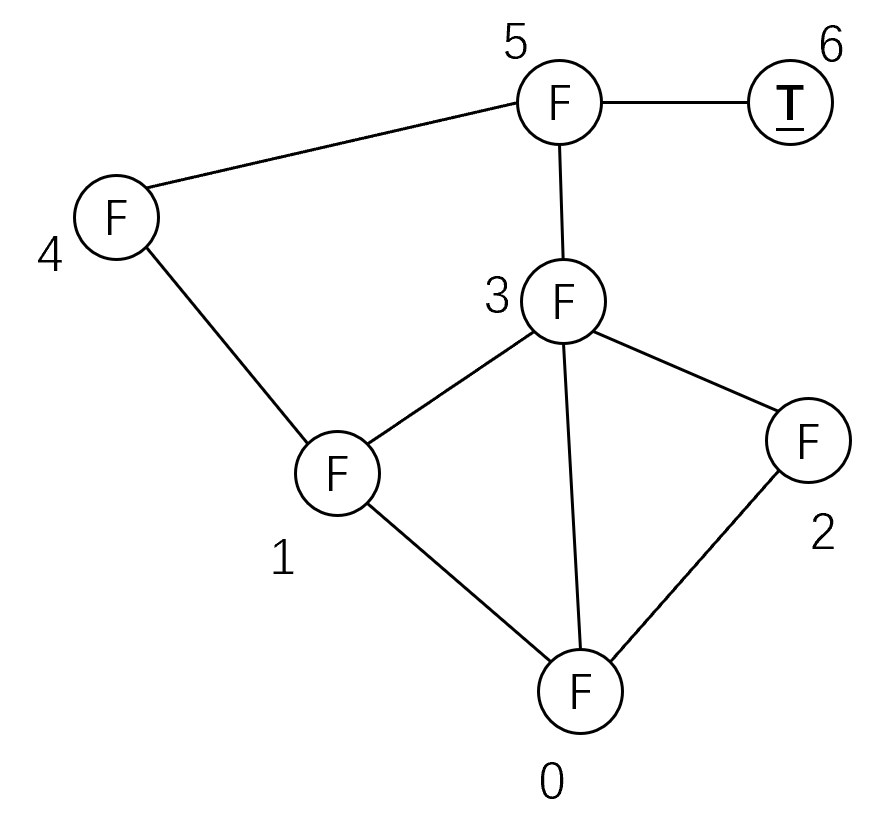
\includegraphics[width=0.37\textwidth]{assets/pics_and_ppts/ch5/习题07救出维火女.png}
\end{center}

\begin{cppcode}
    const int N/* = 7 */;
    
    char trees[N] /*= {'F', 'F', 'F', 'F', 'F', 'F', 'T'}*/;    // 保存顶点数据
    int Matrix[N][N] /*= {    // 邻接矩阵
        { 0, 1, 1, 1, 0, 0, 0 },
        { 1, 0, 0, 1, 1, 0, 0 },
        { 1, 0, 0, 1, 0, 0, 0 },
        { 1, 1, 1, 0, 0, 1, 0 },
        { 0, 1, 0, 0, 0, 1, 0 },
        { 0, 0, 0, 1, 1, 0, 1 },
        { 0, 0, 0, 0, 0, 1, 0 },
    }*/;
    
    void FindPath(int u) {

    }
\end{cppcode}

\vspace{\baselineskip}


*17. 若上题条件下，假设所有灵魂通路的通行时间\textbf{相等}，当樱花树可以抵达时，要求输出所有可行路径中距离最短的一条（经过的边数最少的），不可抵达时同样
输出“......”，请写出代码。

若有多条路径最短，任意输出一条即可。\\


\label{other:DFS求最短路径}
*18. 若16题条件下，假设所有灵魂通路的通行时间\textbf{不等}，当樱花树可以抵达时，要求输出所有可行路径中距离最短的一条（花费时间最少的），不可抵达时同样
输出“......”，请写出代码。

若有多条路径最短，任意输出一条即可。邻接矩阵中已存储了各灵魂通路的通行时间。
\begin{cppcode}
    const int N/* = 7 */;
    
    char trees[N] /*= {'F', 'F', 'F', 'F', 'F', 'F', 'T'}*/;    // 保存顶点数据
    int Matrix[N][N] /*= {    // 邻接矩阵，0表示无路，非0表示通行时间
        { 0, 3, 2, 2, 0, 0, 0 },
        { 3, 0, 0, 2, 5, 0, 0 },
        { 2, 0, 0, 1, 0, 0, 0 },
        { 2, 2, 5, 0, 0, 6, 0 },
        { 0, 1, 0, 0, 0, 2, 0 },
        { 0, 0, 0, 6, 2, 0, 1 },
        { 0, 0, 0, 0, 0, 1, 0 },
    }*/;
    
    void FindPath(int u) {

    }
\end{cppcode}

\vspace{\baselineskip}

19. （某年408真题）已知无向连通图存在EL路径的充要条件是度为奇数的顶点数为0或2。
设无向连通图$G$采用邻接矩阵存储，类型定义如下：
\begin{cppcode}
    typedef struct {
        int numVertices, numEdges;  // 图中实际的顶点数和边数
        char VerticesList[MAXV];    // 顶点表。MAXV为已定义常量
        int Matrix[MAXV][MAXV];       // 邻接矩阵
    }MGraph;
\end{cppcode}

若顶点$i$到$j$存在边，则Edge[i][j]为1，否则为0。请设计算法int IsExistEL(MGraph G)，判断$G$是否存在EL路径，若存在，返回1，否则返回0。要求：\\
1）给出算法的基本设计思想；\\
2）根据设计思想，采用C或C++语言描述算法，关键之处给出注释；\\
3）说明你所设计算法的时间和空间复杂度。\\

20. （某年408真题）已知通常将有向图中出度大于入度的顶点称为K顶点。若图采用邻接矩阵存储，类型定义如下：
\begin{cppcode}
    typedef struct {
        int numVertices, numEdges;  // 图的顶点数和有向边数
        char VerticesList[MAXV];    // 顶点表，MAXV为已定义常量
        int Matrix[MAXV][MAXV];       // 邻接矩阵
    }MGraph;
\end{cppcode}
若顶点$i$到$j$存在边，则Edge[i][j]为1，否则为0。请你设计一个算法int PrintKVertices(MGraph G)，输出G中的所有K顶点，并返回K顶点的个数。要求：\\
1）给出算法的基本设计思想；\\
2）根据设计思想，采用C或C++语言描述算法，关键之处给出注释。\\




\end{exercise}
\clearpage

\begin{exerciseanswer}
1. 选B。顶点A与顶点E存在相互连通的路径: A -> D -> E 以及 E -> D -> A，选项B错误。\\

2. 选D。A项，存在两顶点A、E，A到E无路径，所以$G_1$不是强连通的；对于$G_2$，F到G无路径，因此$G_2$不是强连通的；$G_3$任意两顶点之间都有路径，是强连通的。B项，
图$G$存在以下强连通分量：
\begin{center}
    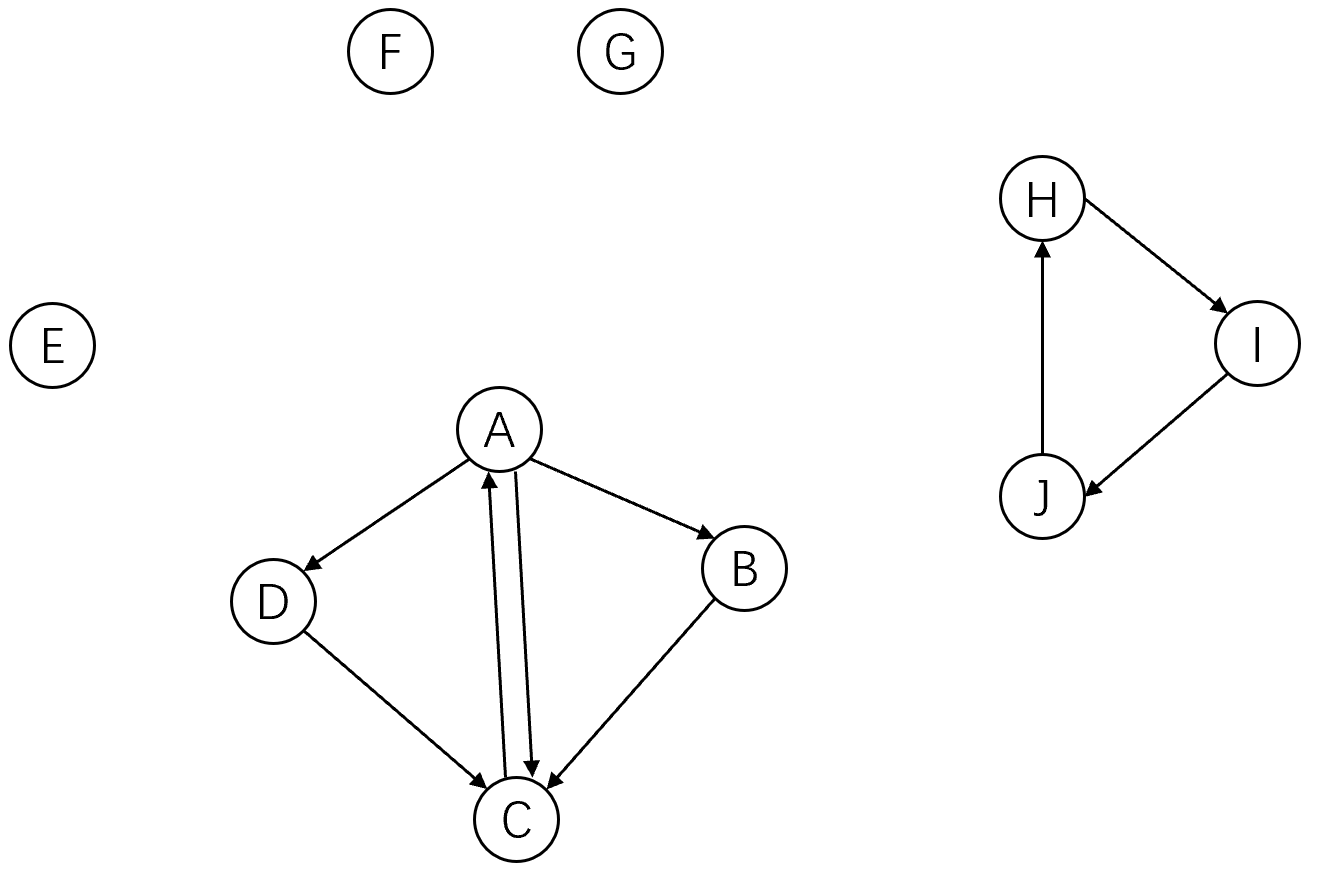
\includegraphics[width=0.58\textwidth]{assets/pics_and_ppts/ch5/习题02，图的基本概念答案图.png}
\end{center}
显然数量大于3。C项，顶点A出度为3，入度为1，C正确。D项，顶点F出度为0，入度为1，D错误。\\

3. 选A。下图所示的图是一个无向连通图，但不具有\(\mathrm{II}\)与\(\mathrm{III}\)的特性。只有\(\mathrm{I}\)正确。
\begin{center}
    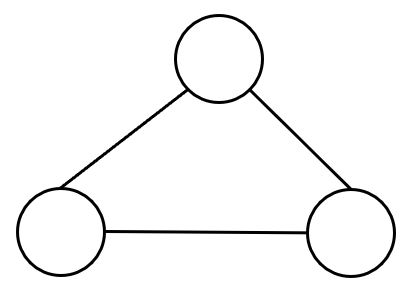
\includegraphics[width=0.19\textwidth]{assets/pics_and_ppts/ch5/习题03，09408无向连通图特性答案图.png}
\end{center}

\vspace{\baselineskip}

4. 要使得边数达到最大，一定是任意两个顶点之间都有一条边。因此最大边数是从N个顶点选出2个的组合数：
\[
    C_N^2 = \frac{N(N-1)}{2}
\]

另一种理解方式：第1个顶点可以与另外N-1个顶点各形成一条边，共N-1条；第2个顶点可以和剩下的N-2个顶点各
形成一条边，共N-2条......第N-1个顶点可以和剩下的1个顶点组成1条边，此时，任意两个顶点都有边存在了，达到最大。因此最大边数为
\[
    (N-1) + (N-2) + ... + 2 + 1 = \frac{(N-1)(1+N-1)}{2} = \frac{N(N-1)}{2}
\]

事实上，对于不存在重复边、不存在自环（即指向自身的边）的图，通常称其为\term{简单图}。若无特殊说明，
本书中提到的所有图均为简单图。

对于有N个顶点的无向图，其边数最大为\(\frac{N(N-1)}{2}\)，
有\(\frac{N(N-1)}{2}\)条边的无向图就被称为\term{完全图}，也被称为\term{简单完全图}，完全图中的任意两个顶点之间均存在边。
而对于有向图，显然边数最大为\(2\cdot  \frac{N(N-1)}{2} = N(N-1)\)，因此，将有\(N(N-1)\)条边的有向图称为\term{有向完全图}，
有向完全图中的任意两个顶点之间都存在方向相反的两条边。\\

5. 要保证连通性，边数最少的情况就是“用一根线将所有顶点串起来”，如图所示：
\begin{center}
    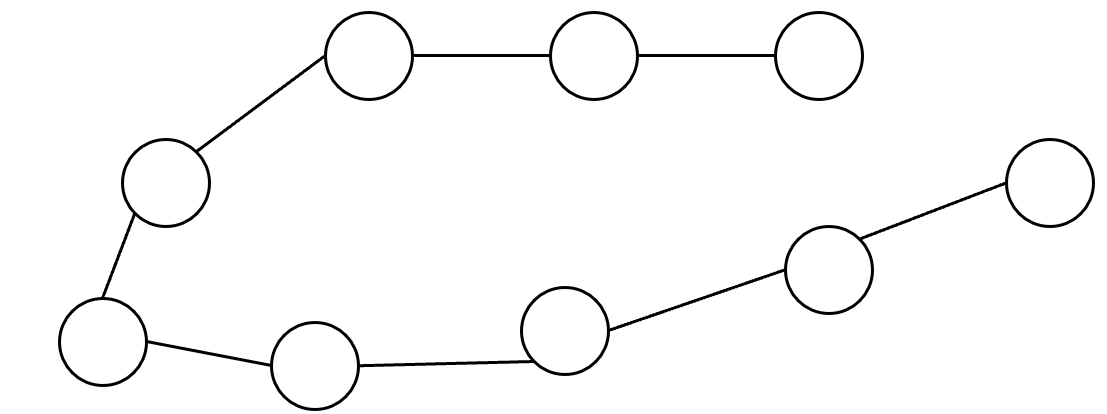
\includegraphics[width=0.52\textwidth]{assets/pics_and_ppts/ch5/习题04，N个顶点的连通图最少边数答案.png}
\end{center}
在此情况下，再少一条边，则图将不连通。显然此情况边数等于顶点数减一。即：\textbf{有N个顶点的无向图，要保证它是连通图，至少要有N-1条边。换句话说，
有N个顶点的无向图，若边数小于N-1，则它一定是不连通的。}

也可以这样理解：对于N个顶点、无边的无向图，显然有N个连通块。之后每添加1条边，一定能让两个本不连通的块连通起来。因此，添加N-1条边后，就只剩一个连通块了。\\

6. 选C：16。若N为15，则存在一种方式：将其中6个顶点通过这\(\frac{6\cdot (6-1)}{2} = 15\)条边连接为一个完全图，将第七个顶点孤立在外，使得图G不连通。而若N为16，
多出来的一条边一定可以让第七个顶点与另外6个连通。\\

7. 选A。图的邻接矩阵AdjM[i][j]存储的是编号为$i$的顶点到编号为$j$的顶点的边的信息。0表示无边，那么编号为$i$的顶点的度
就等于邻接矩阵第 \(i\) 行（或第 \(i\) 列）中非零元素的数量。\\

8. 选B。 如果是有向图，那么AdjM[i][*]，即第$i$行的非0元素数量，是顶点$i$的出度，而AdjM[*][i]，即第$i$列的非0元素数量，是顶点$i$的入度，二者加起来才是顶点$i$的度。\\

9. 选C。邻接表存储方式，为每个顶点维护一个线性表，存放其所有\term{出边}的信息，顶点A有3条出边，顶点C有1条出边，选C。\\

10. 选D。D项序列\{E,C,D,A,B\}，探索完前两个顶点E、C，与C邻接的顶点尚有A未被访问，仍可以向更深处探索，而序列中下一个探索了D，说明不是深度优先的策略。\\

11. 选C。本题意在更直观地揭示树的层序遍历与图的广度优先遍历之间的关联。它们都是像涟漪一样从中心向外“扩散”：
\begin{center}
    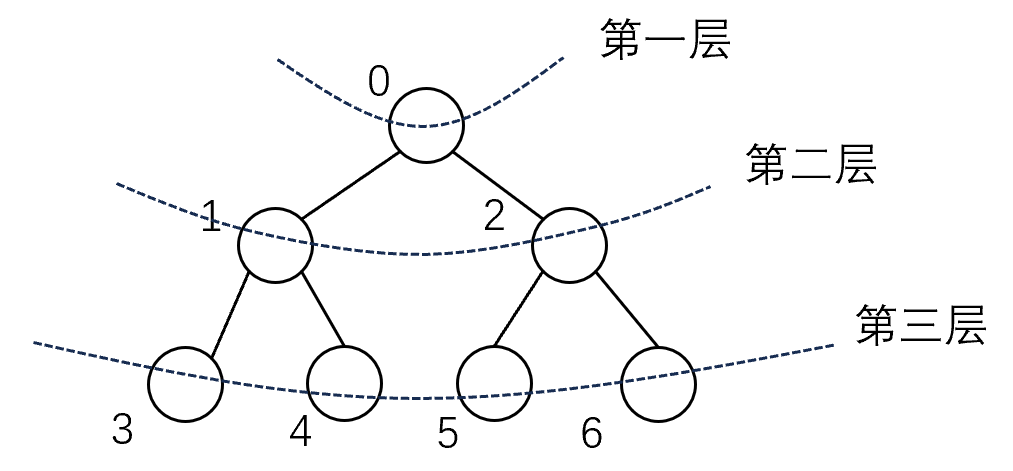
\includegraphics[width=0.39\textwidth]{assets/pics_and_ppts/ch5/习题06，树上的广度优先答案图.png}
\end{center}

12. 选A。广度优先是越早看见的顶点越先被访问，是“先进先出”的，因此通常用队列实现，而不是栈；深度优先是“后进先出”的，通常用栈实现，A错误。\\

13. 1）邻接矩阵版：
\begin{cppcode}
    bool AdjM[N][N];    // 假设该数组已经正确存储了G的邻接矩阵
    // 返回所有顶点的度数之和
    int DegreeSum(int N) {
        // 在此处完成你的代码
        int ret = 0;
        for(int i=0; i<N; i++) {
            for(int j=0; j<N; j++) {
                if(AdjM[i][j] == 1) {
                    ret += 1;
                }
            }
        }
        return ret;
    }
    
\end{cppcode}

2）邻接表版：
\begin{cppcode}
    vector<int> AdjList[N]; // 该数组已经正确存储了G的邻接表
    // 返回所有顶点的度数之和
    int DegreeSum(int N) {
        // 在此处完成你的代码
        int ret = 0;
        for(int i=0; i<N; i++) {
            ret += AdjList[i].size();
        }
        return ret;
    }
\end{cppcode}

事实上，对于无向图，一条边必定连接两个顶点，为这两个顶点各贡献一个度。因此，无向图中所有顶点的度数之和一定是图的边数的 2 倍。这个事实被称为\term{“牵手定理”}。

类似地，对于有向图，一条有向边始于一个顶点（贡献 1 个出度）、终于一个顶点（贡献 1 个入度），因此有向图中所有顶点的出度之和
（或入度之和）等于图的边数 $M$，而有向图的总度数之和（入度 + 出度）同样是边数的 2 倍（$2M$）。\\



14. 显然，本题从起点出发，DFS遍历一遍，每访问到一个新的顶点，就将计数器加一即可。
“访问”一个节点的过程就是将全局计数器加一的过程，而不需要对顶点自身做任何其他操作。代码如下：
\begin{cppcode}
    const int N/* = 100*/;
    bool visited[N];    // 已初始化为false

    void DFS(int v, int& count, vector<int> AdjList[N]) {
        count += 1;
        visited[v] = true;
        for(int i=0; i<AdjList[v].size(); i++) {
            int adj_vertex = AdjList[v][i];
            if(!visited[adj_vertex]) {
                DFS(adj_vertex, count, AdjList);
            }
        }
    }

    int CountAccessibleTrees(vector<int> AdjList[N]) {
        int count = 0;
        // 从起点0出发，全局计数器count以引用传递，每访问一个顶点时计数。
        DFS(0, count, AdjList);
        return count;
    }
\end{cppcode}

\vspace{\baselineskip}

15. 这是非常经典的求图的连通块的问题。我们检查一遍图的所有顶点（代码中的循环\Circled{1}），若其没被访问过，说明这是一个新的需要计数的连通块，
于是计数加一，并以该顶点为起点执行BFS或DFS，将该连通块的所有顶点标记为已访问。反之若顶点已被访问，说明它属于之前遍历过的某
个连通块，已经被计数过了，跳过即可。
\begin{cppcode}
    const int N/* = 100*/;
    bool visited[N];    // 已初始化为false

    // 以v为起点，遍历v所在的连通块
    void BFS(int v, vector<int> AdjList[N]) {
        queue<int> q;
        q.push(v);
        visited[v] = true;
        while(!q.empty()) {
            int cur_vertex = q.front();
            q.pop();
            for(int i=0; i<AdjList[v].size(); i++) {
                int adj_vertex = AdjList[cur_vertex][i];
                if(!visited[adj_vertex]) {
                    q.push(adj_vertex);
                    visited[adj_vertex] = true;
                }
            }
        }
    }

    int CountConnectedComponents(vector<int> AdjList[N]) {
        int count = 0;
        for(int i=0; i<N; i++) {    // 循环@\Circled{1}@
            if(!visited[i]) {   // 该顶点所在的连通块没被计数过
                count += 1;
                BFS(i, AdjList);
            }
        }
        return count;
    }
\end{cppcode}

\vspace{\baselineskip}

*16. 本题思路比较简单，通过BFS或DFS从起点开始搜索，当搜索到'T'时即找到了一条路径。问题在于搜索过程中如何将涉足过的轨迹记录下来？

\Circled{1}对于递归的DFS代码，算法一定是一步一个脚印地，沿着合法路径在前进或回溯。当走进一条错误的路径之后，
如何正确地进行\term{回溯}？如图所示，
\begin{center}
    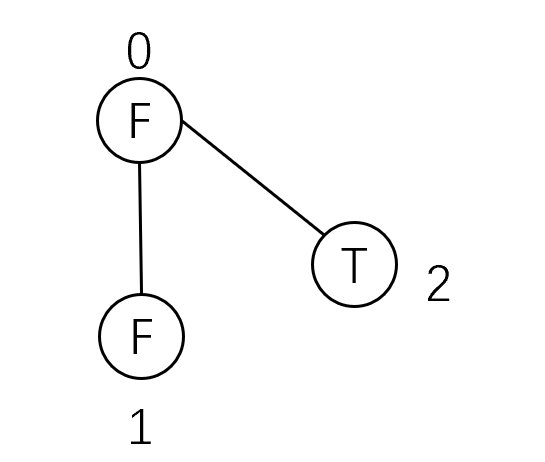
\includegraphics[width=0.23\textwidth]{assets/pics_and_ppts/ch5/习题08，任意路径答案图.png}
\end{center}
若从0出发进入了1，此时记录的路径是“01”，回到0后，要将路径回溯到“0”。显然，由于回退时总是将“\uline{后}路过的顶点\uline{先}从路径中拿掉”，因此可以使用一个
栈保存所经过的路径。回溯时，将顶点从栈顶弹出即可。

\Circled{2}而对于非递归的BFS或DFS代码，不同的是，非递归算法的下一个“出发点”是由队列（或栈）中元素决定的，顶点的访问顺序未必是一条
合法路径。所以对于非递归代码，要记录路径，可以设一个Pre[]数组，如Pre[3]值为0就表示顶点3的上一步是顶点0。

我们给出非递归的BFS与递归的DFS代码如下：
\begin{cppcodeNum}[codetitle={非递归的BFS解法}]
    const int N/* = 7 */;
    char trees[N] /*= {'F', 'F', 'F', 'F', 'F', 'F', 'T'}*/;    // 保存顶点数据
    int Matrix[N][N] /*= {    // 邻接矩阵
        { 0, 1, 1, 1, 0, 0, 0 },
        { 1, 0, 0, 1, 1, 0, 0 },
        { 1, 0, 0, 1, 0, 0, 0 },
        { 1, 1, 1, 0, 0, 1, 0 },
        { 0, 1, 0, 0, 0, 1, 0 },
        { 0, 0, 0, 1, 1, 0, 1 },
        { 0, 0, 0, 0, 0, 1, 0 },
    }*/;
    int Pre[N]; // 记录路径
    bool visited[N];
    
    // 以v为起点，BFS搜索一条找到'T'的路径。若找到了，返回'T'所在顶点的编号。若'T'不可达，返回-1。
    int BFS(int v) {
        queue<int> q;
        int ret = -1;
        if(trees[v] == 'T') {
            return v;
        }
        q.push(v);
        visited[v] = true;
        while(!q.empty()) {
            int step = q.front();
            q.pop();
            for(int i=0; i<N; i++) {
                if(Matrix[step][i] != 0 && !visited[i]) {
                    // 记录轨迹的上一个顶点编号
                    Pre[i] = step;
                    if(trees[i] == 'T') {
                        ret = i;
                        return ret;
                    }
                    q.push(i);
                    visited[i] = true;
                }
            }
        }
        return ret;
    }

    void FindPath(int u) {
        for(int i=0; i<N; i++) {
            Pre[i] = -1;
            visited[i] = false;
        }
        int flower_idx = BFS(u);
        if(flower_idx == -1) {
            cout << "......" << endl;
            return;
        }
        // 从flower_idx向前找到的路径顶点顺序是反的，用一个栈正向打印
        stack<int> to_print;
        for(int i=flower_idx; i!=-1; i=Pre[i]) {
            to_print.push(i);
        }
        while(!to_print.empty()) {
            cout << to_print.top();
            to_print.pop();
        }
        cout << endl;
    }
\end{cppcodeNum}
以上BFS算法要访问约$N$个顶点，访问每个顶点时要遍历该顶点的邻接矩阵以找出邻接点，时间为$O(N)$，因此总的时间复杂度为$O(N^2)$。

递归的DFS代码：
\begin{cppcodeNum}[codetitle={递归的DFS解法}]
    const int N/* = 7 */;
    char trees[N] /*= {'F', 'F', 'F', 'F', 'F', 'F', 'T'}*/;    // 保存顶点数据
    int Matrix[N][N] /*= {    // 邻接矩阵
        { 0, 1, 1, 1, 0, 0, 0 },
        { 1, 0, 0, 1, 1, 0, 0 },
        { 1, 0, 0, 1, 0, 0, 0 },
        { 1, 1, 1, 0, 0, 1, 0 },
        { 0, 1, 0, 0, 0, 1, 0 },
        { 0, 0, 0, 1, 1, 0, 1 },
        { 0, 0, 0, 0, 0, 1, 0 },
    }*/;
    // 存在解返回true，否则返回false
    bool DFS(int v, stack<int>& track, bool visited[]) {
        visited[v] = true;
        track.push(v);  /* 先假设经由该顶点v能到达樱树，在轨迹中记录此顶点，若后面发现无法到达，回溯。 */
        bool solved = false;    // 先假设不存在解，若递归过程中找到了樱树，将结果一层一层地向上带。
        if(trees[v] == 'T') {
            solved = true;
            return solved;
        }
        
        // 从此顶点v开始，向邻接点递归地探索
        for(int i=0; i<N; i++) {
            if(!visited[i] && Matrix[v][i] == 1) {
                // 以此顶点v为（半路）起点，可以找到樱树，返回true
                if(DFS(i, track, visited) == true) {
                    solved = true;
                    return solved;
                }
            }
        }
        /* 若代码执行至此，说明事实上由此顶点v作为（半路）起点的所有路径均无法找到樱树，于是从轨迹中弹出此顶点，回溯到上一个顶点，继续探索其他路径。 */
        track.pop();
        return solved;
    }

    void FindPath(int u) {
        // 动态记录轨迹
        stack<int> track;
        bool visited[N];
        for(int i=0; i<N; i++) {
            visited[i] = false;
        }
        // 存在解
        if(DFS(u, track, visited) == true) {
            // 栈中保存的轨迹是相反的，保存到一个vector中之后从后向前打印
            vector<int> to_print;
            while(!track.empty()) {
                to_print.push(track.top());
                track.pop();
            }
            for(int i=to_print.size()-1; i>=0; i--) {
                cout << to_print[i];
            }
            cout << endl;
        } else {    // 不存在解
            cout << "......" << endl;
        }
    }
\end{cppcodeNum}
该算法的性能瓶颈在于DFS，最坏情况下，假设每个顶点都有接近N个邻接点，则DFS被调用接近N次，并且每次调用执行接近N次循环，因此算法最坏时间复杂度为$O(N^2)$。

\vspace{\baselineskip}

*17. 事实上，{\color{red}\textbf{上题}}的非递归BFS解法，求出来的那条路径一定是最短路径。为什么？


如图所示，由于 BFS 总是先搜索完当前层的所有顶点，才会进入下一层，因此它一定会按照从近到远的顺序发现顶点。
所以当 BFS 第一次发现某个顶点时，就已经找到了从起点到达该顶点、经过边数最少的路径。
\begin{center}
    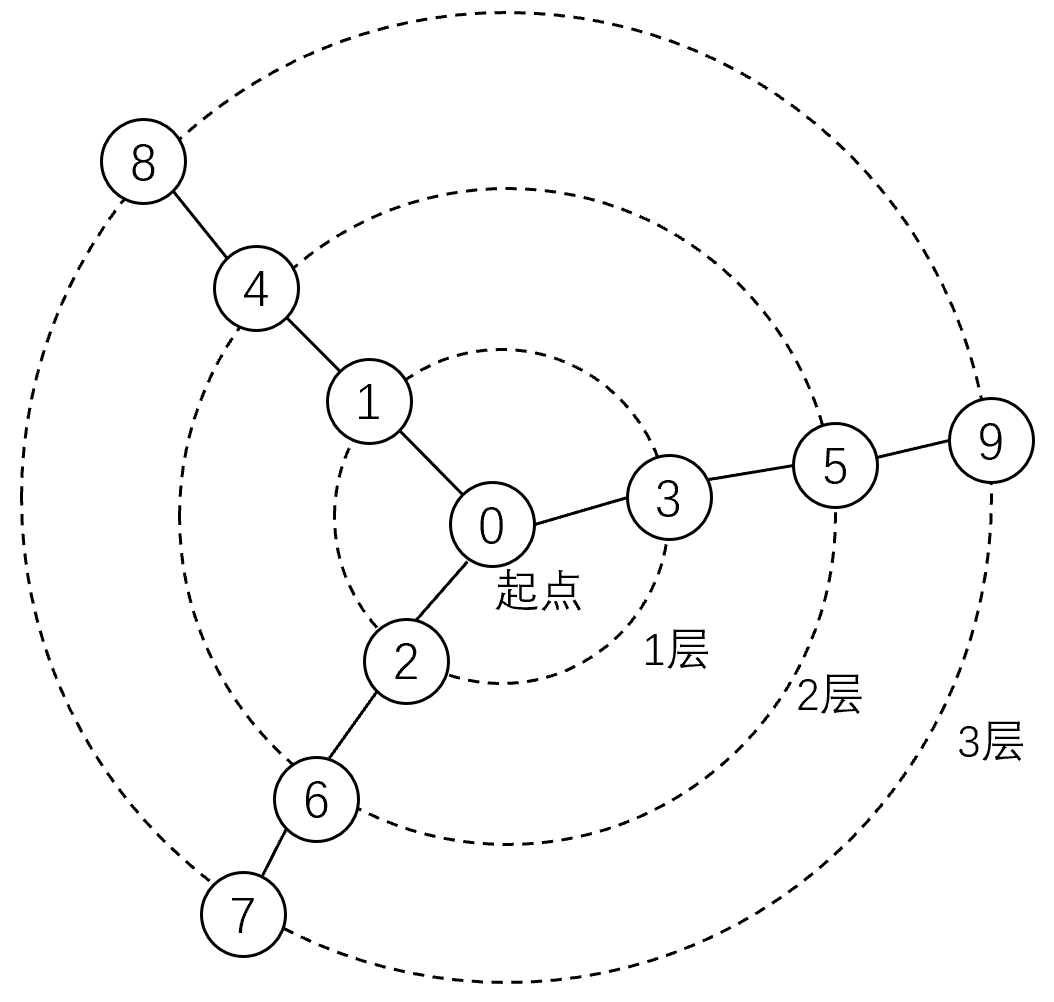
\includegraphics[width=0.45\textwidth]{assets/pics_and_ppts/ch5/21BFS求解最短路径原理.png}
\end{center}

\textbf{当图中所有边的权重都相同时，路径的总权重只取决于它经过了多少条边。而 BFS 恰好能够保证：第一次到达某个顶点时，经过的边数最少。
因此对于无权图或等权图，BFS可以用于求解\uwave{最短路径}问题。}

而对于带权图，经过的边数最少的路径不一定是总长度最短的路径。因此BFS算法无法求解带权图的最短路径。而DFS可以将所有的路径都探索一遍，通过穷举路径的方式计算出
路径最短的是哪一条。因此通过DFS方式穷举路径的方法，是一种求带权图最短路径的算法，我们将在{\color{red}\textbf{下一题中体会}}。\\



*18. 如{\color{red}上题所述}，对于带权图无法使用BFS求解最短路径，但是可以DFS递归地将所有路径穷举一遍。
在搜索到\textquotesingle T\textquotesingle 后回溯，继续寻找其他路径。
一种简单的想法是，在DFS过程中，将当前已经找到的每一条路径轨迹及其长度都记录下来，最后再选择一条长度最短的输出其轨迹。我们做如下定义：
\begin{cppcode}
    // 定义一条路径
    struct track {
        stack<int> nodes;   // 轨迹序列，如0356
        int length;         // 该路径的长度
    };
    track t;    // 当前走过的路径
    vector<track> tracks;   // 用于保存所有路径
\end{cppcode}
于是我们可以在DFS递归过程中动态维护当前走过的路径t（包括轨迹顶点集nodes以及轨迹的长度length），
当找到\textquotesingle T\textquotesingle 时，就将当前记录的路径t放入tracks尾部：
\begin{bulk}
    tracks.push\_back(track);
\end{bulk}

需要注意的是，在寻找路径的过程中，每个顶点有可能被多次访问，因此回溯时不仅要维护t.nodes与t.length，还要将当前节点重新标记为未访问。比如在下图中，
假设已经找到了一条路径01356，回溯时若不把这些顶点的visited[]标记为false，会导致后面重新从0出发时，无法达到1和3，从而错过最短路径：“0356”。
\begin{center}
    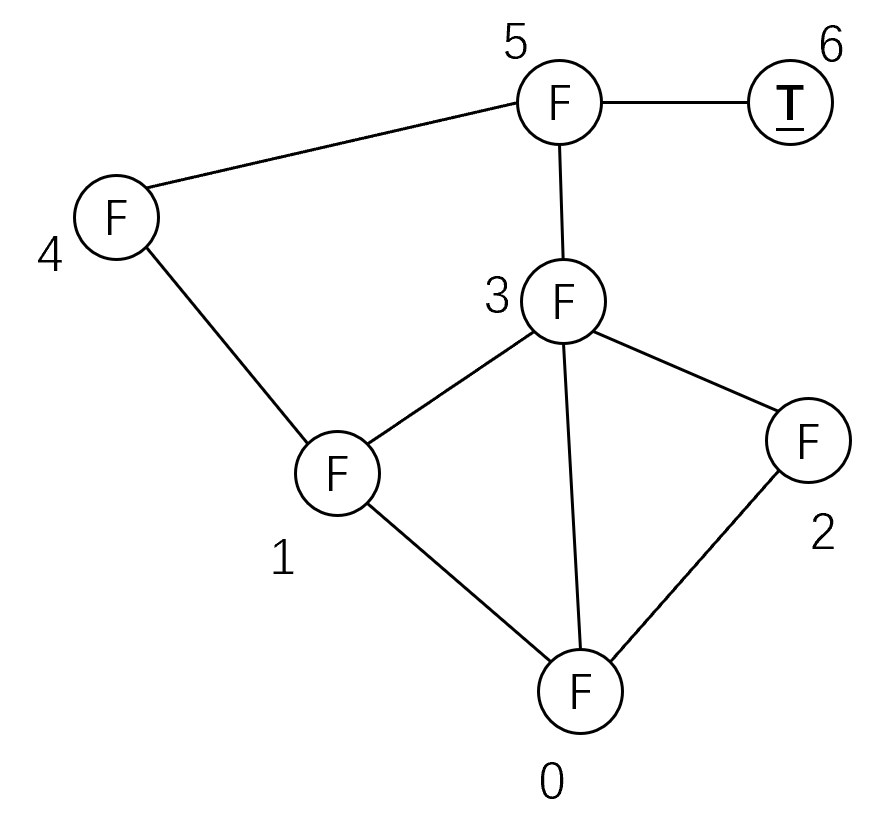
\includegraphics[width=0.30\textwidth]{assets/pics_and_ppts/ch5/习题07救出维火女.png}
\end{center}

完整的代码如下所示。
\begin{cppcode}
    const int N/* = 7 */;
    char trees[N] /*= {'F', 'F', 'F', 'F', 'F', 'F', 'T'}*/;    // 保存顶点数据
    int Matrix[N][N] /*= {    // 邻接矩阵，0表示无路，非0表示通行时间
        { 0, 3, 2, 2, 0, 0, 0 },
        { 3, 0, 0, 2, 5, 0, 0 },
        { 2, 0, 0, 1, 0, 0, 0 },
        { 2, 2, 5, 0, 0, 6, 0 },
        { 0, 1, 0, 0, 0, 2, 0 },
        { 0, 0, 0, 6, 2, 0, 1 },
        { 0, 0, 0, 0, 0, 1, 0 },
    }*/;
    struct track {
        stack<int> nodes;
        int length;
    };

    void DFS(int v, int pre_v, track& t, bool visited[], vector<track>& tracks) {
        visited[v] = true;
        t.nodes.push(v);
        t.length += Matrix[pre_v][v];
        if(trees[v] == 'T') {
            tracks.push_back(t);

            // 回溯
            visited[v] = false;
            t.nodes.pop();
            t.length -= Matrix[pre_v][v];
            return ;
        }

        for(int i=0; i<N; i++) {
            if(Matrix[v][i] != 0 && !visited[i]) {
                DFS(i, v, t, visited, tracks);
            }
        }

        // 回溯
        visited[v] = false;
        t.nodes.pop();
    }

    void FindPath(int u) {
        vector<track> tracks;
        track t;
        bool visited[N];
        for(int i=0; i<N; i++) {
            visited[i] = false;
        }

        DFS(u, u, t, visited, tracks);
        // tracks为空说明从未找到过任何一条路径，不可达。
        if(tracks.empty()) {
            cout << "......" << endl;
        } else {
            // 判断一下哪条路径长度最短
            int min_length = 0x3fffffff;
            int ans_idx = -1;   // 最短路径的下标
            vector<int> min_path;
            for(int i=0; i<tracks.size(); i++) {
                if(tracks[i].length < min_length) {
                    min_length = tracks[i].length;
                    ans_idx = i;
                }
            }
            vector<int> to_print;
            while(!tracks[ans_idx].nodes.empty()) {
                to_print.push_back(tracks[ans_idx].top());
                tracks[ans_idx].pop();
            }
            for(int i=to_print.size()-1; i>=0; i--) {
                cout << to_print[i] ;
            }
            cout << endl;
        }
    }
\end{cppcode}

最坏情况下，假设N个顶点任意两顶点之间都存在边，边的数量达到了$ \frac{N(N-1)}{2} $（{\color{red}\textbf{见本习题第4题}}），从起点出发，下一步有(N-1)条路，
这(N-1)个新的起点，每个起点又有(N-2)条路可以选择，......，于是需要辗转的顶点数量为
\[
    (N-1)\cdot (N-2)... \cdot 2 \cdot 1
\]
时间复杂度为$O(N!)$量级。对于稍微复杂一点的图，这是根本不可能接受的！

事实上，在DFS过程中，可以再维护一个变量，记录当前已经找到的所有可行路径的最短长度，在递归到某顶点时，若此时当前路径长度已经大于最短长度，则无需继续递归下去，而是
直接回溯即可。这种优化策略通常被称为\term{剪枝}，意为在递归树中剪掉一些无意义的路线。

此外，完全可以在DFS搜索过程中只维护和更新“当前已找到的所有路径中最短的那一条路径”，而不必将所有路径都存储起来，这对于存储空间是一个极大的优化。感兴趣的同学
可以自己尝试写出代码。\\

但是，以上两种优化策略也仅仅是杯水车薪，带来的优化比较有限。在\ref{sec:最短路径}节中，我们将介绍一种极具创造性的算法---迪杰斯特拉算法，来解决
\term{单源最短路径问题}。\\

19. 计算所有顶点的度即可。代码如下：
\begin{cppcode}
    int IsExistEL(MGraph G) {
        int odd_deg_num = 0;    // 计算度为奇数的顶点个数
        for(int i=0; i<G.numVertices; i++) {
            int i_degree = 0;   // 计算顶点i的度
            for(int j=0; j<G.numVertices; j++) {
                if(G.Matrix[i][j] == 1) {
                    i_degree += 1;
                }
            }
            if(i_degree%2 == 1) {   // 顶点i是度为奇数的顶点
                odd_deg_num += 1;
            }
        }
        return (odd_deg_num == 0) || (odd_deg_num == 2);
    }
\end{cppcode}
显然时间复杂度为$O(n^2)$，空间复杂度为$O(1)$。

\vspace{\baselineskip}

20. 遍历一遍邻接矩阵，计算各顶点的入度和出度即可。
\begin{cppcode}
    int PrintKVertices(MGraph G) {
        int ret = 0;    // 计算K顶点的个数
        for(int i=0; i<G.numVertices; i++) {
            int out_deg = 0;    // 顶点i的出度
            int in_deg = 0;     // 入度
            for(int j=0; j<G.numVertices; j++) {
                // i到j有路径，i的出度+1
                if(G.Matrix[i][j] != 0) out_deg += 1;   
                // j到i有路径，i的入度+1
                if(G.Matrix[j][i] != 0) in_deg += 1;    
            }
            // 出度大于入度，是一个K顶点，输出
            if(out_deg > in_deg) {
                cout << G.VerticesList[i];
                ret += 1;
            }
        }
        return ret;
    }
\end{cppcode}

\end{exerciseanswer}%%%%%%%%%%%%%%%%%%%%%%%%%%%%%%%%%%%%%%%%%%%%%%%%%%%%%%%%%%%%%%%%%%%%%%%%%%%%%%%%%%%%%%%%%%%%%%%%%%%%%%%%%%%%%%%%%%%%%%%%%%%%%%%%%
\section{最短路径}
\label{sec:最短路径}
王国的故事还在继续。根据指挥官给出的遍历方法，信使无一疏漏地将大敌来犯的消息传遍了王国的每一座城池、每一座要塞。士兵和居民们纷纷武装起来，
布起防御系统，准备迎接那场即将到来的大战。

\subsection{迪杰斯特拉算法}
接下来，一位指挥官提出了这样一个问题：若某个据点有重兵来犯，从首都派出军队去该据点支援，走哪条路，能够最快到达？这种求解从某顶点到图中其他所有顶点
的最短路径的问题，后来被称为\term{单源最短路径}问题。

为了解决这个问题，指挥官们将王国建模成了一个无向带权图，边的权表示走此路径需要消耗的时间。如图\ref{fig:最短路径王国地图}所示。
\begin{wrapfigure}{l}{0.35\textwidth}
    \centering
    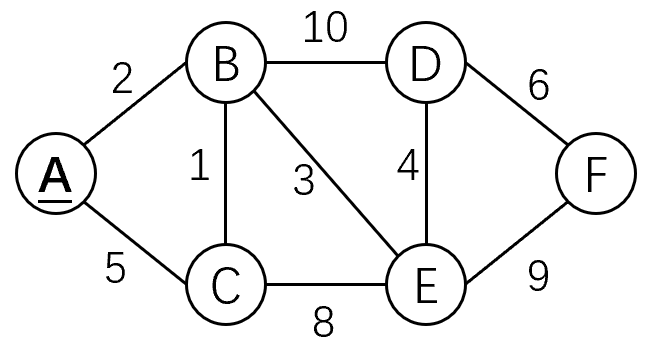
\includegraphics[width=0.35\textwidth]{assets/pics_and_ppts/ch5/10最短路径王国地图.png}
    \caption{}
    \label{fig:最短路径王国地图}
\end{wrapfigure}

假设A为首都，如何求A到F的最短路径？一位指挥官指出，最简单的做法就是把所有可能的路径都找出来，然后比较它们的长度。
这种做法通过DFS进行路径搜索即可实现，如{\color{red}\textbf{习题6第18题}}（
第\pageref{other:DFS求最短路径}页）所做的那样。但是，这种做法存在一个明显的问题：即使其中许多路径已经不可能成为最短路径，我们仍然要花费时间去搜索它们。
对图\ref{fig:最短路径王国地图}进行DFS路径搜索的\uwave{搜索树}如图\ref{fig:DFS搜索树}所示。可以看到每个叶节点即代表了一条路径的终点，
要么是找到了目标顶点，要么是非目标顶点的死路。

\begin{figure}[htbp]
    \centering
    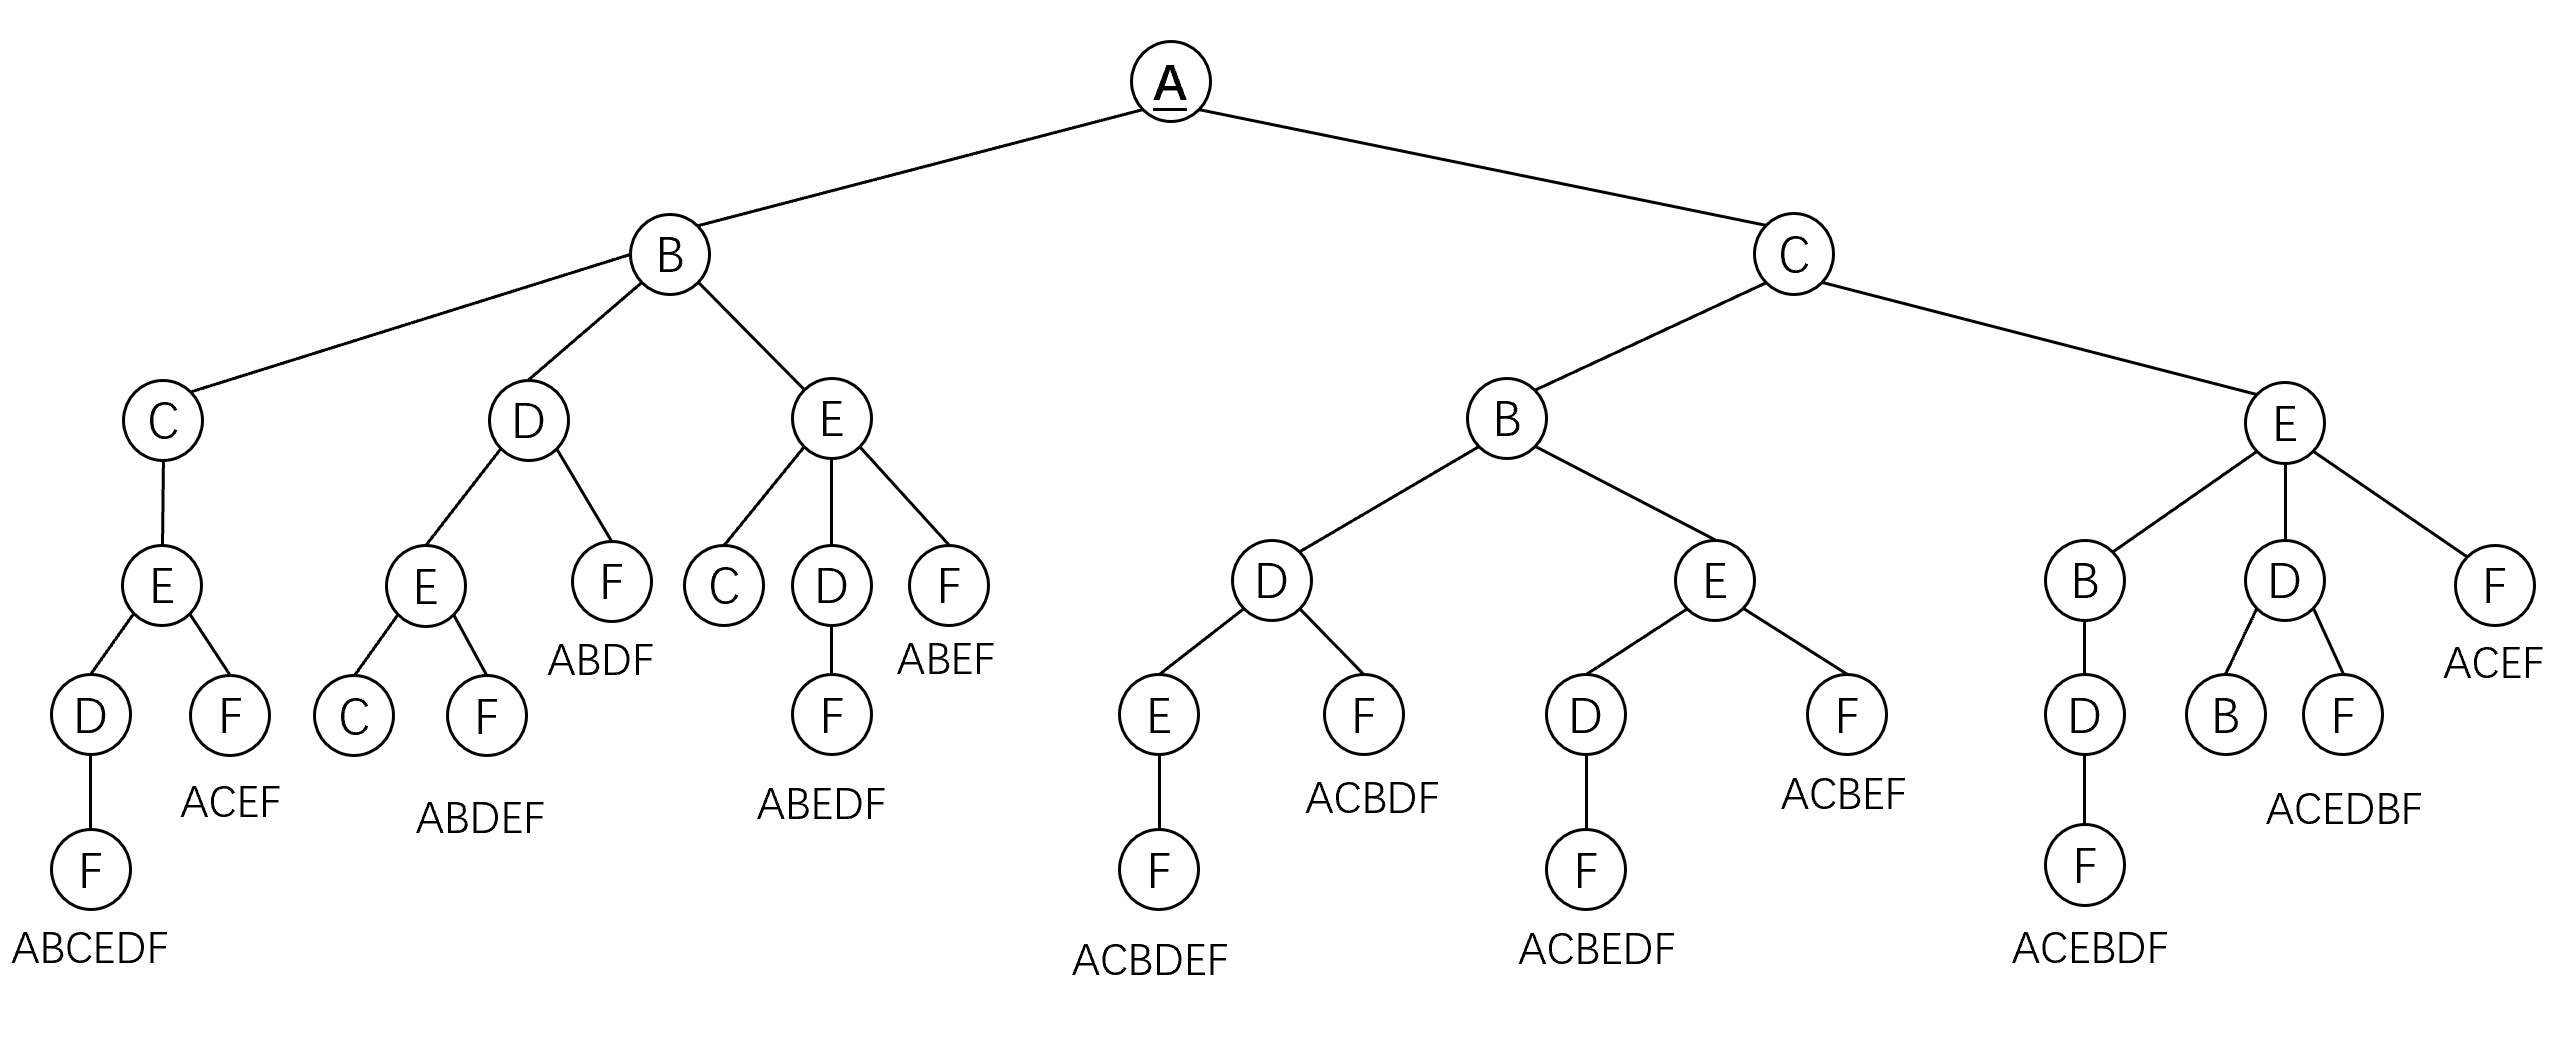
\includegraphics[width=1.05\textwidth]{assets/pics_and_ppts/ch5/11DFS搜索树.png}
    \caption{搜索树}
    \label{fig:DFS搜索树}
\end{figure}

当我们探索到一条可行的路径ABDF时，就已经知道最短路径
不可能大于4，于是ABEDF、ACBDEF等路径其实完全没有必要探索，即使使用\term{剪枝策略}（{\color{red}\textbf{见习题6第18题参考答案}}），
也要至少探索4个顶点再回头。DFS的穷举过程最差时间复杂度是$O(N!)$量级，对于稍微复杂的图，该算法绝对无法接受。况且如果需要求出A到所有顶点的最短路径，就需要
再重复如图\ref{fig:DFS搜索树}的搜索过程若干次。

\begin{notebox}{CoreLoop}
    \hspace{1.6em}我们暂时把思路拉回现实世界。
    
    \hspace{1.6em}执笔至此，笔者以为，接下来要介绍的迪杰斯特拉算法，大抵是本书中最令人惊叹、最具创造性的算法。
    我不想直接介绍迪杰斯特拉算法的过程与实现。我要尝试做一件事情：与你一起思考并探索迪杰斯特拉算法“诞生”的过程：当DFS绝对无法接受时，最短路径问题就摆在我们面前，
    我们将会有哪些思考和结论？以此过程，一方面加深大家对于算法的理解和记忆（而不是枯燥地记住这复杂的过程），另一方面，通过探索过程中的艰难到最后的柳岸花明，
    来体会算法开创者非凡的创造力，以此向艾兹赫尔·迪杰斯特拉（Edsger W. Dijkstra）---这位计算机领域的传奇人物致敬。

    \hspace{1.6em}\textbf{如你对此过程兴趣无多，请直接跳至\bookmarkref{bookmark:waypoint-8}{waypoint-8}处，这不会影响后面的旅途。}
\end{notebox}

首先，我们很容易想到这样一个想法：

\textbf{假设顶点$\boldsymbol{i}$正确的事实最短路径为$\boldsymbol{mind[i]}$}，那么，一定有：
\[
    mind[i] = min( mind[j_1] + cost(j_1, i), mind[j_2] + cost(j_2, i), ..., mind[j_n] + cost(j_n, i) )
\] 
其中，\(j_1, j_2, ..., j_n\)为$i$的所有邻接点，\(cost(j, i)\)表示顶点$j$到$i$的花费。
\begin{wrapfigure}{l}{0.30\textwidth}
    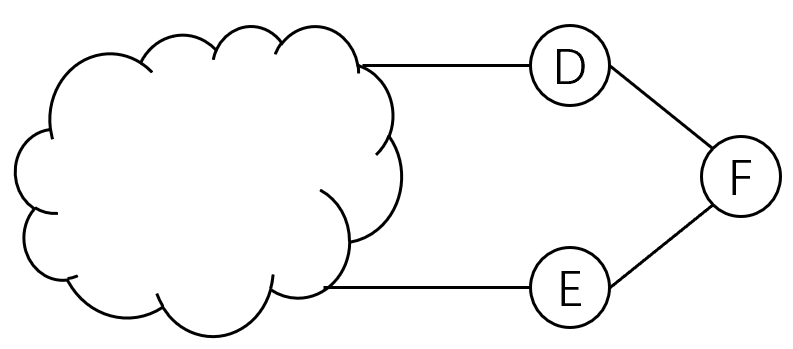
\includegraphics[width=0.30\textwidth]{assets/pics_and_ppts/ch5/13到达F必然经过D和E.png}
\end{wrapfigure}
例如如图\ref{fig:最短路径王国地图}中，要到达F，必然经过D或E，因此对于顶点F，一定有：
\[
    mind[F] = min( mind[D] + cost(D, F), mind[E] + cost(E, F) )
\]

也就是说，F的最短路径就是\Circled{1} A到D的最短路径 + D到F的花费 与 \Circled{2} A到E的最短路径 + E到F的花费 这二者之间更小的。
以上是\textbf{第一个事实}。那么只要确定了D、E的最短路径，F的最短路径也就确定了。

那么我们能不能先确定某些顶点的最短路径呢？\\

显然，顶点A到自身的花费（即$mind[A]$）一定是能确定的：就是0。这是因为路程花费时间不可能为负，所以A -> xxx -> A的花费一定更大。我们将这种
思想记为\textbf{“不绕弯思想”}。

同时，知道了mind[A]为0之后，对于顶点C，他有A、B、E三个邻接点，因此有：
\[
    mind[C] = min( mind[A] + cost(A, C), mind[B] + cost(B, C), mind[E] + cost(E, C) )
\]
其中的\(mind[A] + cost(A, C)\)这一项就能计算得出：\(0 + 5 = 5\)。于是我们可以记录下
来\textbf{当前已知的（并非全局的）C的最短路径$\boldsymbol{cur\_mind[C]} = 5$}，并在未来
某时刻确定了B、E的\(mind[B]\)和\(mind[E]\)时，若\(mind[B] + cost(B, C) < cur\_mind[C]\) 或 \(mind[E] + cost(E, C) < cur\_mind[C]\)，则可以用B或E
来更新\(cur\_mind[C]\)，这样最终得到的\(cur\_mind[C]\)一定是全局最短路径。于是我们顺着这个思路会自然地有这样的想法：\textbf{在确定了一个顶点的全局最短
路径mind[]时，要尝试更新其所有邻接点的最短路径，否则可能错过正确解。}

于是在知道了\(mind[A]\)之后我们更新所有A能到达的邻接点的“当前最短路径\(cur\_mind[]\)”，此时：
\begin{bulk}
    \begin{center}
        $cur\_mind[B] = 2$ \\
        $cur\_mind[C] = 5$
    \end{center}
\end{bulk}
而其他顶点暂未找到一条到达A的路径。如图\ref{fig:思考版迪杰斯特拉算法过程} a）所示，带下划线的数字表示该顶点当前已知的最短路径$cur\_mind[]$，
顶点有填充则表示该顶点的全局事实最短路径已经确定。
\begin{figure}[htbp]
    \centering
    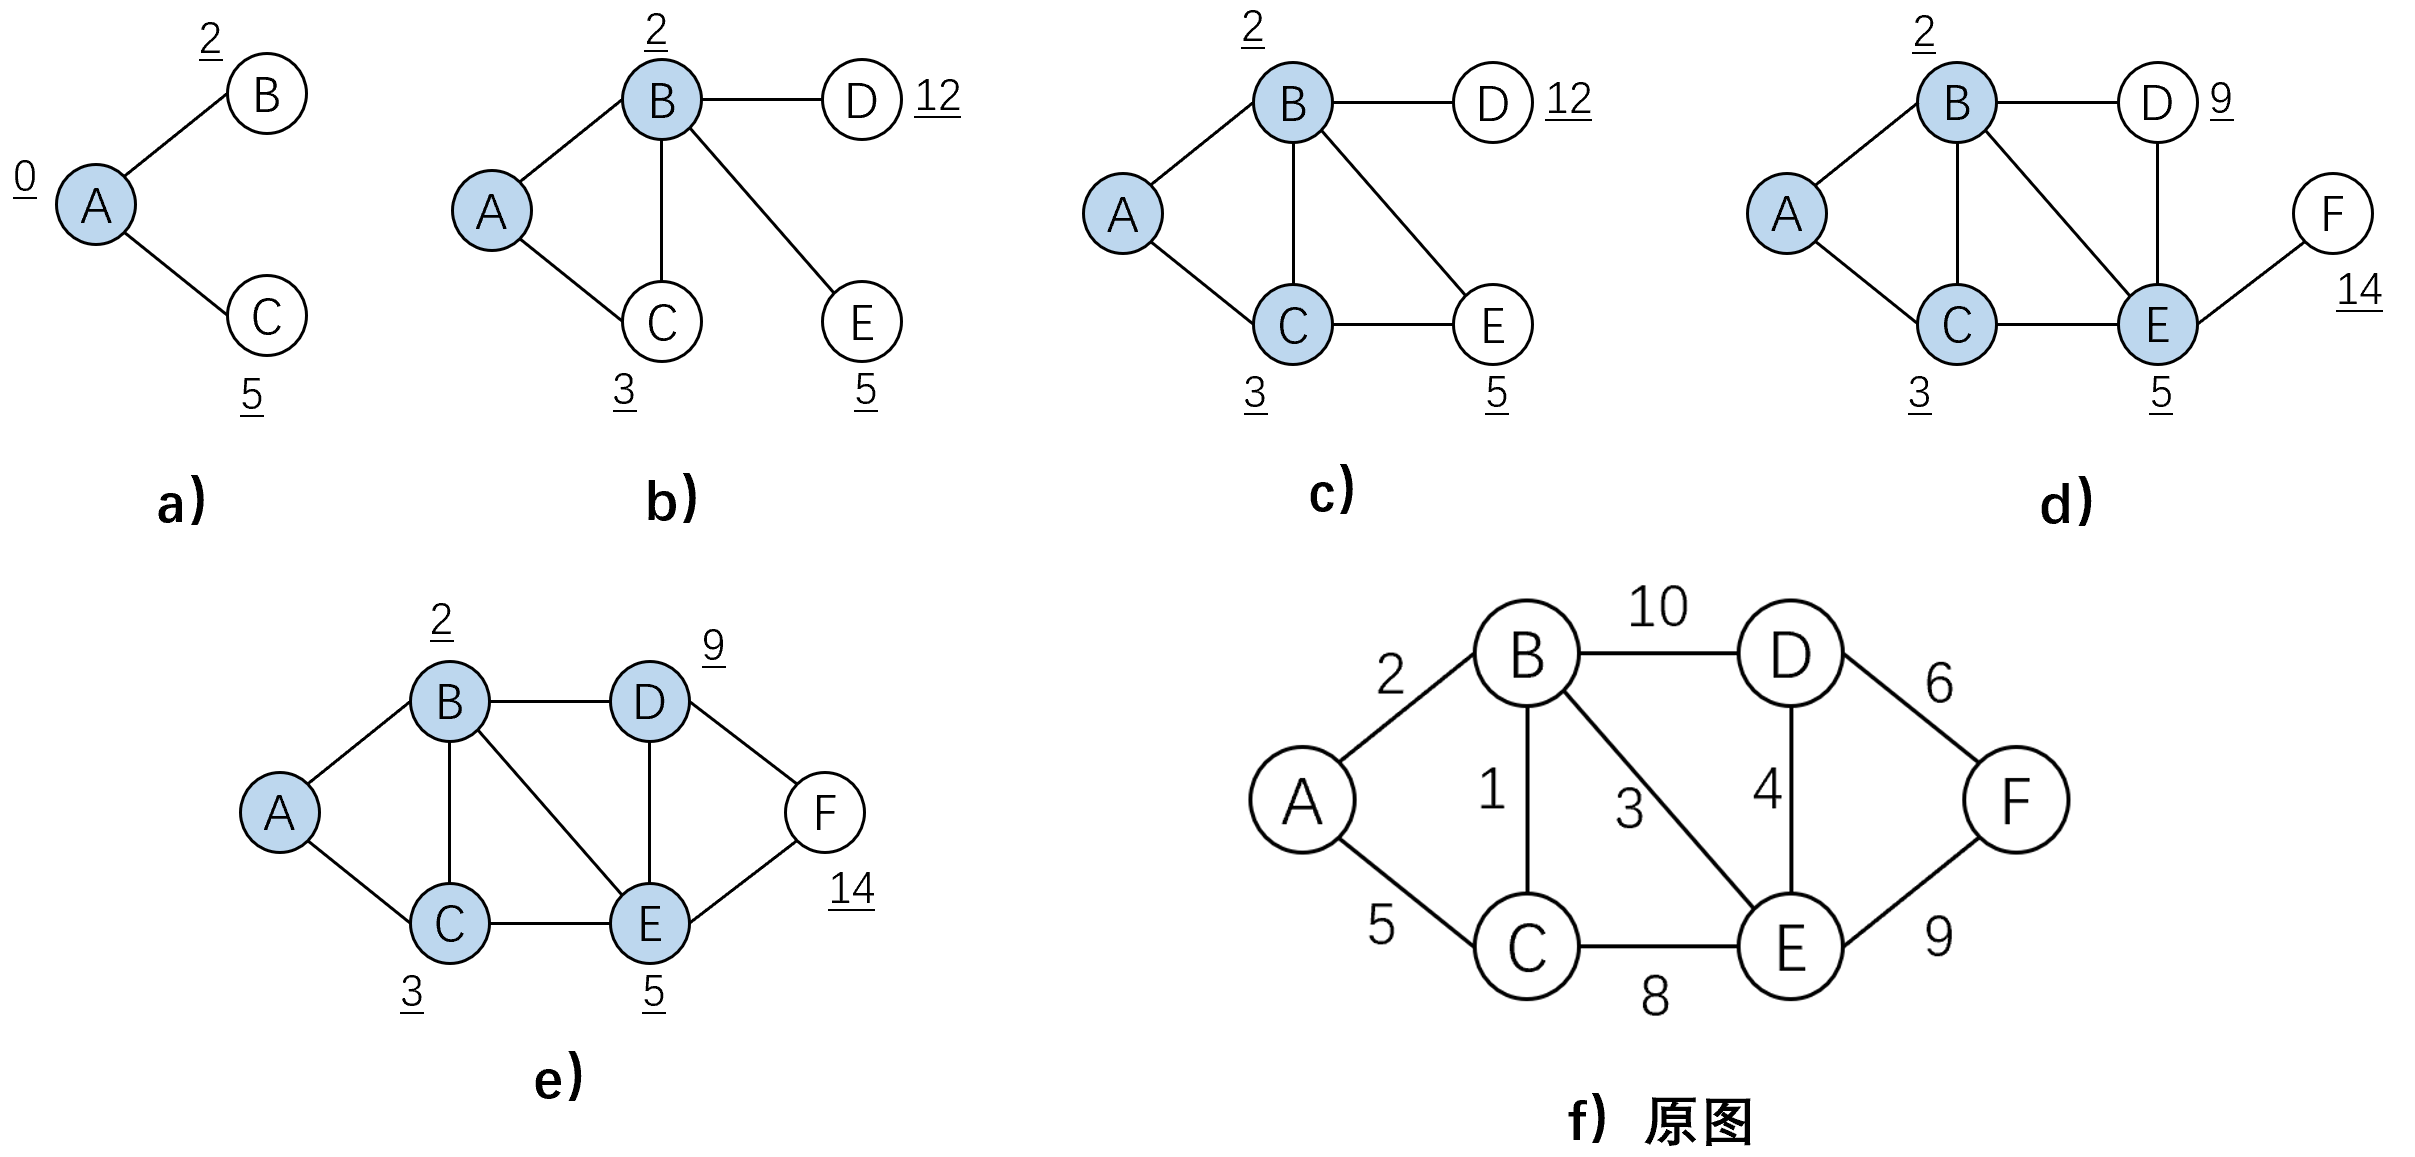
\includegraphics[width=0.99\textwidth]{assets/pics_and_ppts/ch5/12思考版迪杰斯特拉算法过程.png}
    \caption{}
    \label{fig:思考版迪杰斯特拉算法过程}
\end{figure}

我们会发现，此时\(cur\_mind[B] = 2\)一定是B的全局最短路径（因为B是所有A的邻接点中花费最小的那个，因此 A -> B 一定
比 A -> 非B 更短，结合“不绕弯思想”，B此时一定全局最短）。我们用集合$S$记录已经找到全局最短路径的顶点，此时
\[
    S = \{A, B\}
\]
如前所述，确定了$mind[B]$后，就可以更新与B邻接的C、D、E的当前已知最短路径$cur\_mind[]$信息：
\begin{bulk}
        $cur\_mind[C] = min(5, mind[B] + cost(B, C)) = min(5, 2+1) = 3$\\
        $cur\_mind[D] = mind[B]+cost(B,D) = 2 + 10 = 12$\\
        $cur\_mind[E] = 2 + 3 = 5$
\end{bulk}
如图\ref{fig:思考版迪杰斯特拉算法过程} b）所示。此时所有$cur\_mind[]$中，最小的就是$cur\_mind[C]$。根据“不绕弯思想”，显然此时C已知的当前最短一定
也是全局最短。可是，如何证明？接下来这部分便是迪杰斯特拉算法最为精彩也是最难理解的部分，还请听我慢慢道来。\\


如何证明当前已知的所有最短路径$cur\_mind[]$中最小的那个一定就是该顶点的全局最短路径？

如图\ref{fig:思考版迪杰斯特拉算法过程} b）所示，
由于A、B已确定全局最短路径，C还未确定，且所有可以到达C的路径中一定至少存在一个还未确定的顶点（至少有一个C还未确定），
我们假设\uline{存在}某条路径PATH到C的距离比$cur\_mind[C]$更短：
\begin{bulk}
    \begin{center}
        PATH: A -> xxx -> P -> X -> xxx -> C
    \end{center}
\end{bulk}
我们用X表示路径PATH中的第一个尚未确定全局最短路径的顶点，则它的前一个顶点P的全局最短路径一定已经确定。记这条路径PATH的长度为$L\_PATH$，
则我们实际上假设了
\[
    L\_PATH < cur\_mind[C]
\]
接下来，我们来一点一点证出该假设与事实相悖，从而推翻该假设。

由于P的全局最短路径已经确定，因此$cur\_mind[X]$一定已经由P点更新过，即此时一定有：
\[
    cur\_mind[X] <= mind[P] + cost(P, X)  \quad \text{\textbf{// 式（1）}}
\]
上不等式右边即是假设的那条路径PATH到X时的长度（A -> xxx -> P -> X的长度）。而由于图没有负权边，因此
\begin{bulk}
    A -> xxx -> P -> X
\end{bulk}
的长度一定小于等于
\begin{bulk}
    A -> xxx -> P -> X -> xxx -> C
\end{bulk}
的长度，即下式一定成立：
\[
    mind[P] + cost(P, X) <= L\_PATH    \quad \text{\textbf{// 式（2）}}
\]

于是整理式1式2，有：
\[
    cur\_mind[X] <= mind[P] + cost(P, X) <= L\_PATH   \quad \text{\textbf{// 式（3）}}
\]

而事实上C、X均是此时未确定最短路径的顶点，且C是所有$cur\_mind[]$中最小的那个，因此一定有：
\[
    cur\_mind[C] <= cur\_mind[X] \quad \text{\textbf{// 式（4）}}
\]
由式3、式4，得：
\[
    cur\_mind[C] <= cur\_mind[X] <= mind[P] + cost(P, X) <= L\_PATH
\]
这与我们假设的$L\_PATH < cur\_mind[C]$相悖，因此假设不成立，即不存在一条路径，其距离比当前已知的C的
最小距离$cur\_mind[C]$更小。

\textbf{由以上的过程，我们就证明了：当前已知的所有最短路径$cur\_mind[]$中最小的那个一定就是该顶点的全局最短路径。}\\

于是，接下来的思路就豁然开朗了：不断地选择当前已知的所有最短路径中最小的那个，作为该顶点的全局最短路径（已由上面的过程证明这是绝对正确的），接下来，
以该顶点为新的“中介”，去尝试更新其所有邻接点的$cur\_mind[]$，不断重复这个过程，直至所有顶点的全局最短路径都被确定。我们从C开始，看一遍接下来的过程。
\begin{figure}[htbp]
    \centering
    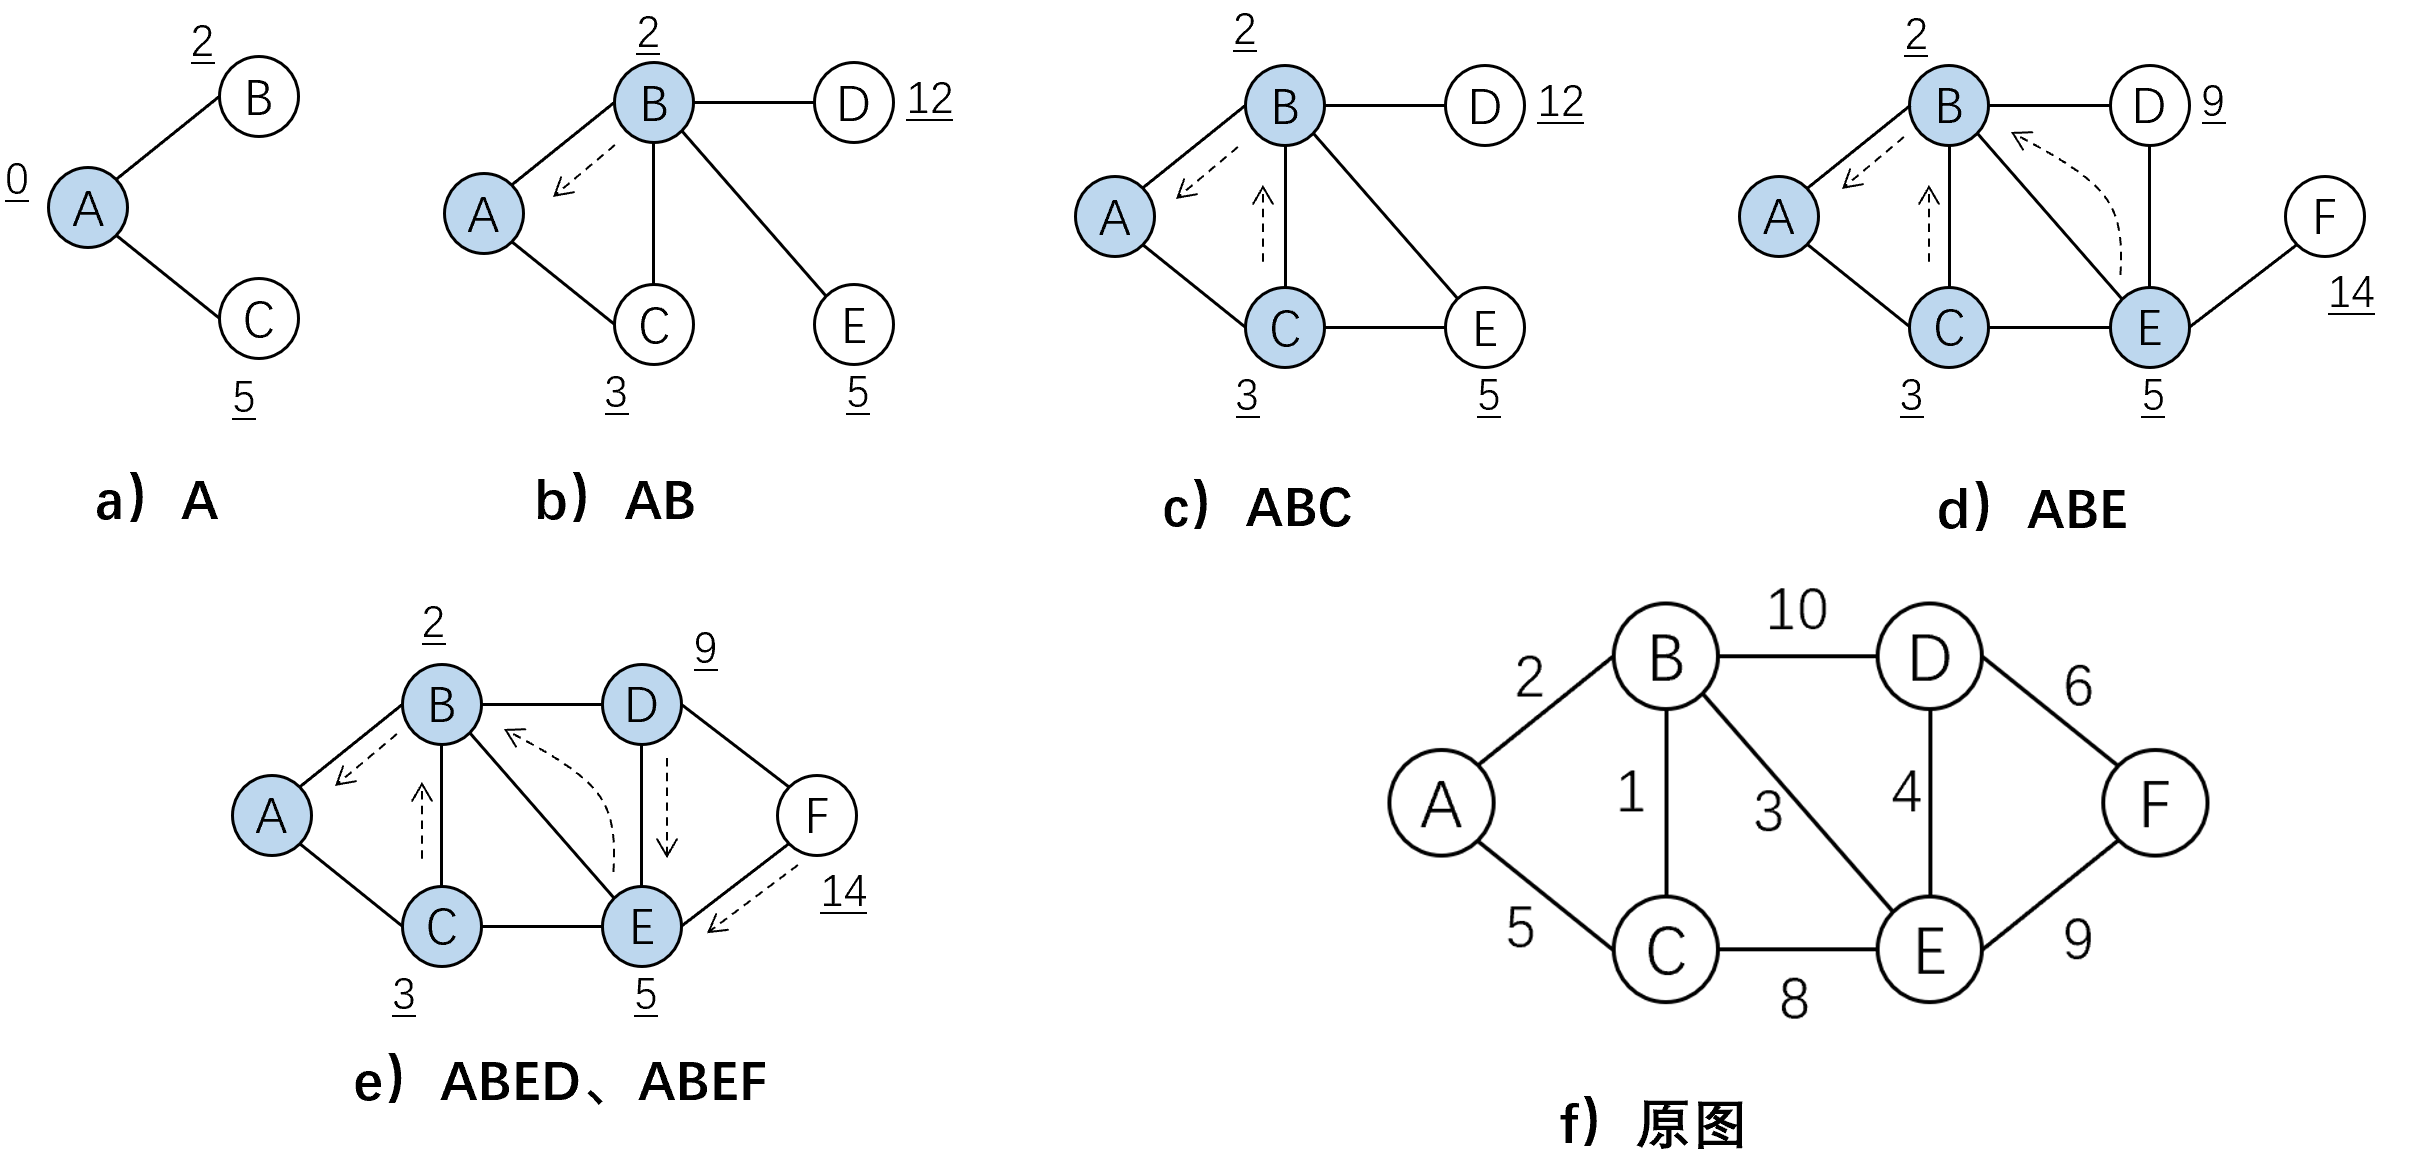
\includegraphics[width=0.99\textwidth]{assets/pics_and_ppts/ch5/14思考版迪杰斯特拉，带路径回溯.png}
    \caption{}
    \label{fig:思考版迪杰斯特拉，带路径回溯}
\end{figure}
如前所述，接下来将C的$cur\_mind[C]$作为C的全局最短，C也就成了“已求解”的顶点。所有已求解的顶点集合S就变成了：
\[
    S = \{A, B, C\}
\]
并且尝试更新$cur\_mind[E]$，但发现通过C到达E的距离：3 + 8 = 11不会比当前已知的：A -> B -> E（5）更短，因此$cur\_mind[E]$依然是5。如图
\ref{fig:思考版迪杰斯特拉，带路径回溯} c）所示。这一次我们在图中加入了路径回溯，记录每一个顶点最终的最短路径是由哪个顶点作为“中介”更新来的，如B
是由A更新来的，因此指向A，C是由B最终更新来的，因此指向B，以此方法记录最短路径本身（B是A -> B, C是A -> B -> C）。


继续从图中的 c）开始，此时$cur\_mind[D]=12$， $cur\_mind[E]=5$，最小的是$cur\_mind[E]$，因此E“已成功求解”，记$mind[E] = cur\_mind[E] = 5$，
并以E作为新的中介，计算：
\begin{bulk}
    $mind[E] + cost(E, D) = 5 + 4 = 9$，小于当前的$cur\_mind[D] = 12$，于是更新D\\
    $mind[E] + cost(E, F) = 5 + 9 = 14$，发现了一条新的到达F的路，所以更新F
\end{bulk}
更新后如图d）所示。最后一步，D作为“已成功求解”的顶点，并作为新的中介尝试更新F，但通过D到F不会更小，因此F的路径前驱依然是E，最终F也已成功求解，无其他顶点
了，如e）所示。

\begin{center}
    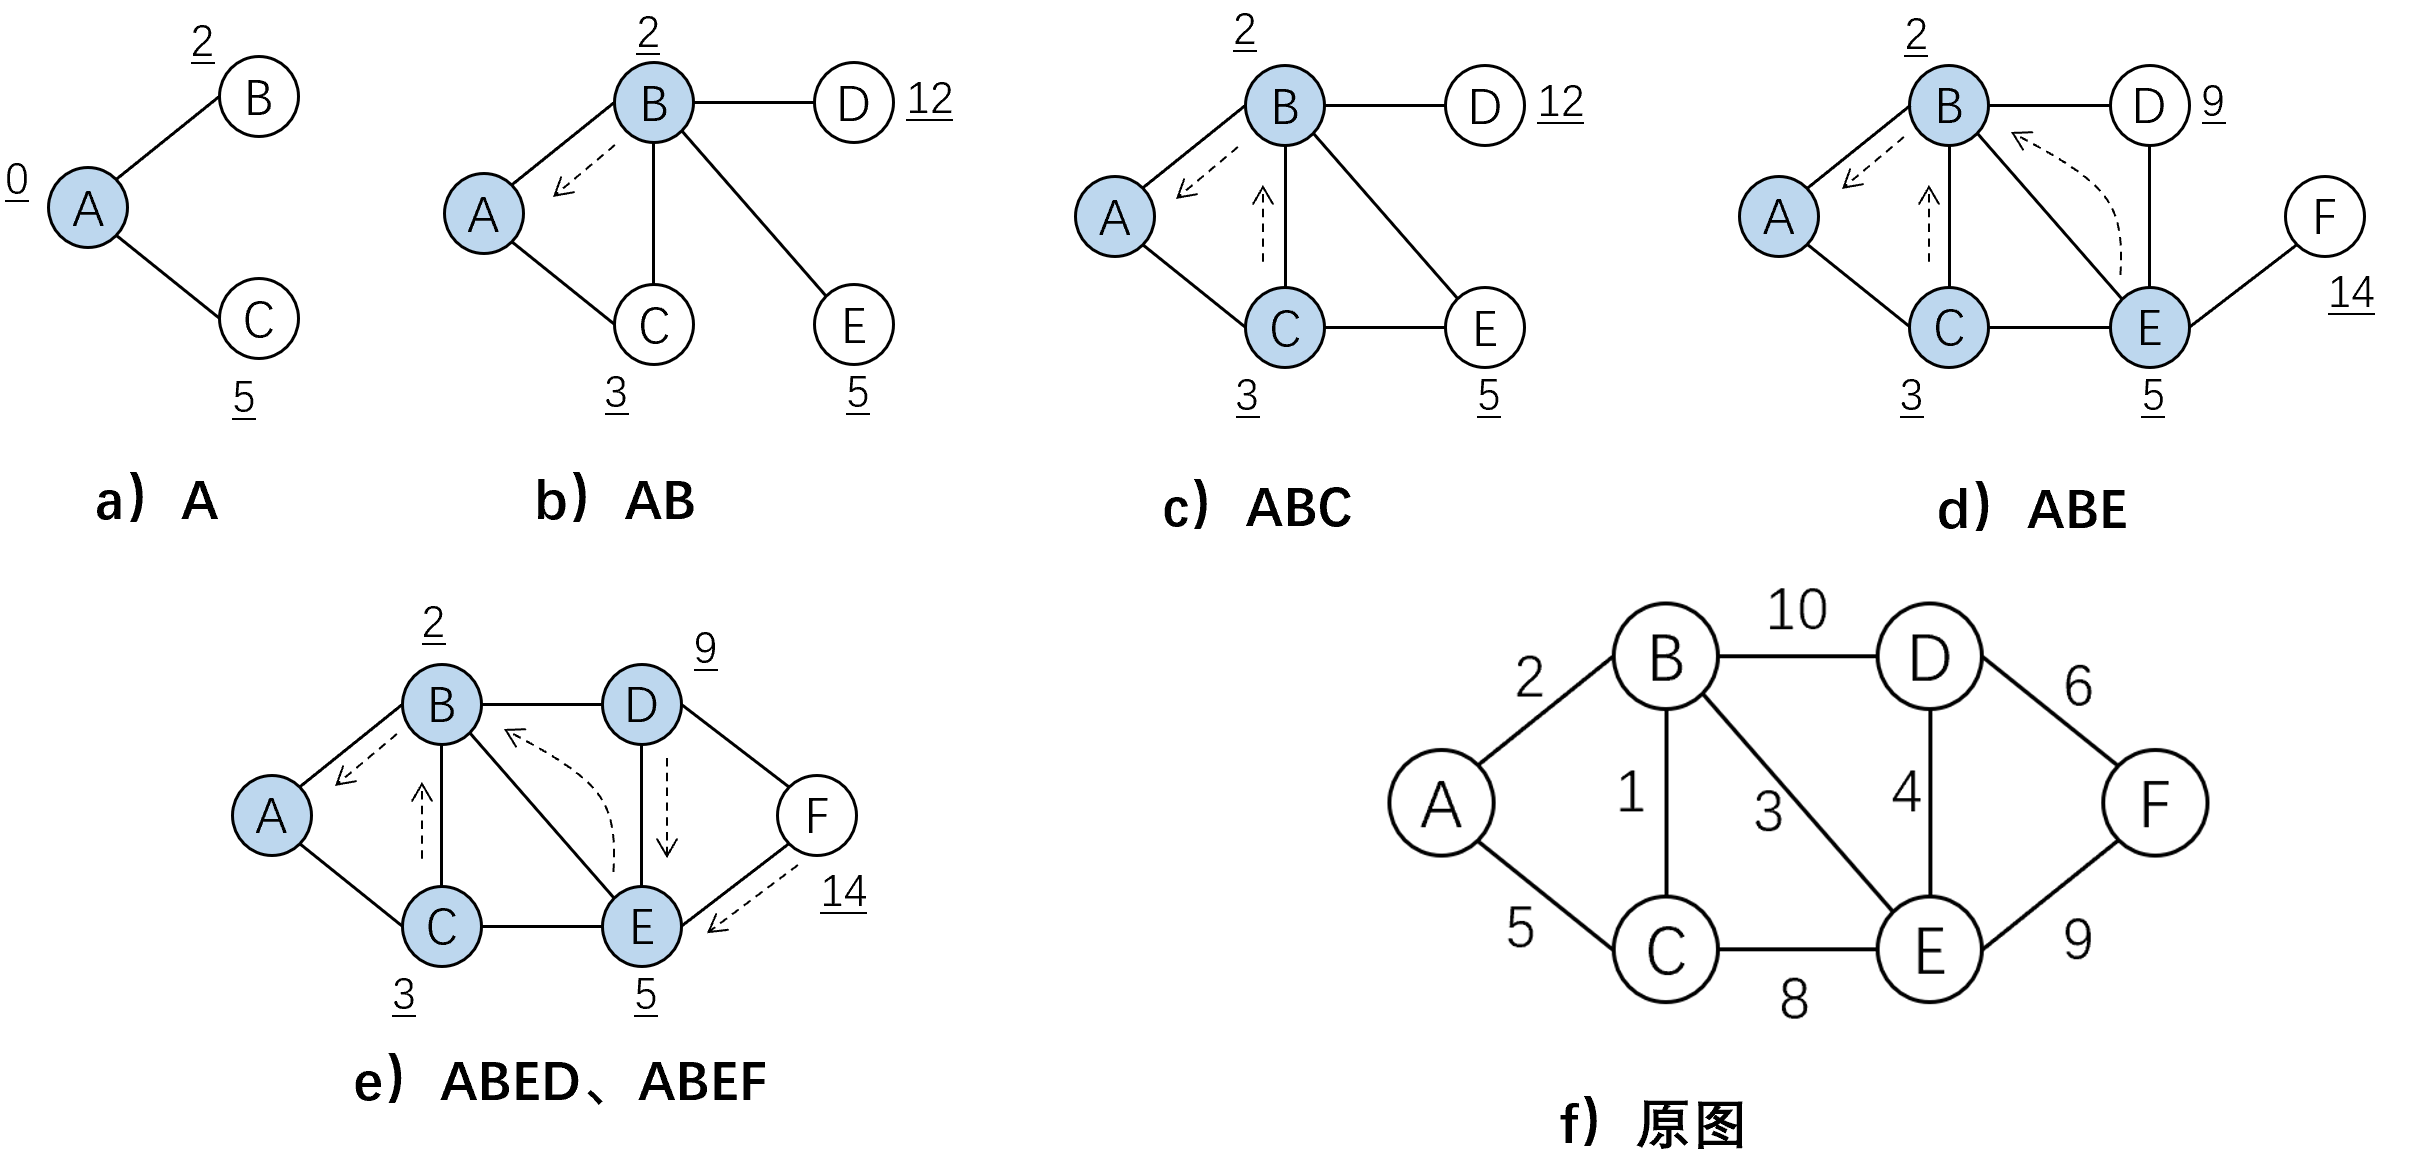
\includegraphics[width=0.99\textwidth]{assets/pics_and_ppts/ch5/14思考版迪杰斯特拉，带路径回溯.png}
\end{center}

至此，所有顶点到达A的最短路径均已求解，$cur\_mind[i]$中最终保存的就是顶点$i$到A的全局最短路径（事实最短路径），因为它一定已经经过了其所有邻接点的更新操作。

最后，需要注意我们以上讨论，都是基于一个假设：图中不存在负权边。通过上述过程也可以看得出来，若存在负边，“不绕弯思想”将不复存在，因此整个推理过程也将崩塌。
正是由于这样的道理，我们马上会看到，\textbf{迪杰斯特拉算法要求图中不存在从源点可达的负权边}。并且由以上思维过程我们知道，若图非连通，
迪杰斯特拉算法也可以得出哪些顶点从源点出发是不可达的。

\bookmark{bookmark:waypoint-8}{waypoint-8}
接下来我们正式介绍赫赫有名的迪杰斯特拉算法（Dijkstra算法）。我们先给出算法正确、完整的步骤，再由一个具体例子直观地感受一下。

\textbf{迪杰斯特拉算法}可用于求解单源最短路径问题。设图$G=(V,E)$有$N$个顶点，$cost(u, v)$为u到v的权值（路径的长度），我们记
$cur\_mind[i]$为顶点$i$当前已知的
最短路径长度，则求解起点$s$到其他任意顶点的最短路径的过程如下：

\begin{enumerate}
    \item 除起点s距离s为0（$cur\_mind[s]=0$）外，当前不知道任何其他顶点到s的最短路径，暂时认为所有顶点的最短路径都是正无穷+inf，将其他所有$cur\_mind[]$初始化为+inf。
    此时所有顶点均\textbf{未求解}。
    \item 从所有\textbf{未求解}顶点中，选出已知的最短路径长度$cur\_mind[]$最小的那个顶点v（第一次选的一定是s），
    该长度一定就是该顶点v到s的全局最短路径长度，于是v\textbf{“已求解”}。
    \item 以v为中介点，尝试更新所有v的邻接点的$cur\_mind[]$。具体来说，对于v的一条指向u的边，若$cur\_mind[v] + cost(v, u) < cur\_mind[u]$，说明经过v
    到u比之前已知的u到s的最短路径更短，所以将$cur\_mind[u]$ 更新为$cur\_mind[v] + cost(v, u)$。这一操作通常被称为\term{“松弛操作”}。
    \item 重复步骤 2 和步骤 3，直到所有可从起点 s 到达的顶点均已确定最短距离。
\end{enumerate}
\textbf{事实上迪杰斯特拉算法就是一个不断地“选点”、“更新”的过程}。我们设置一个数组Solved[]来标记哪些顶点已求解，哪些还未求解；并设立一个数组Pre[]标识每个顶点的路径
前驱，如Pre[1]值为0就表示顶点1的最短路径的上一步是从0走过来的。

我们以图\ref{fig:迪杰斯特拉算法过程演示图} f）所示的图为例来直观地感受一下迪杰斯特拉的过程。
\begin{figure}[htbp]
    \centering
    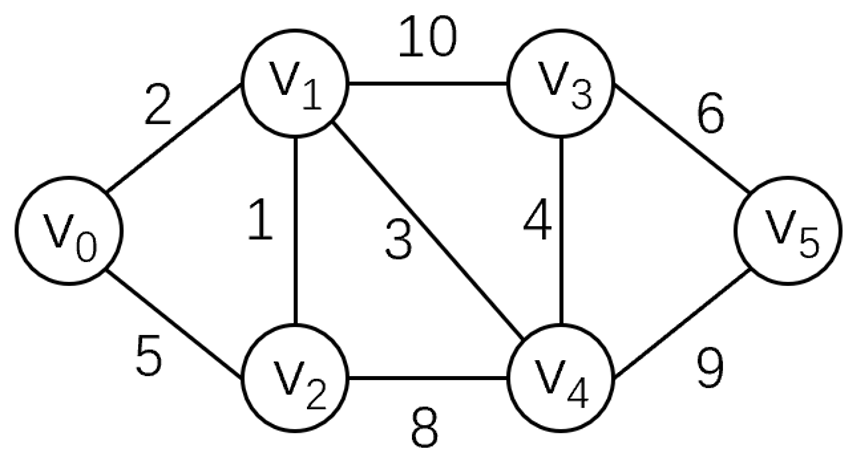
\includegraphics[width=0.40\textwidth]{assets/pics_and_ppts/ch5/15迪杰斯特拉算法过程演示.png}
    \caption{迪杰斯特拉算法过程演示图}
    \label{fig:迪杰斯特拉算法过程演示图}
\end{figure}

我们将$v_0$作为源点s，初始时，所有顶点均未求解，Solved[]为false，除源点s的$cur\_mind[0]=0$外，
所有其他顶点$cur\_mind[]$都是+inf，并且所有顶点的Pre[]均初始化为-1，表示尚未找到一条路径，暂无前驱，如表\ref{table:迪杰斯特拉算法过程演示}“初始”所示。
\begin{enumerate}
    \item
    \begin{minipage}[t]{0.65\linewidth}
        \vspace{0pt}
        从未求解顶点集合
        \{0,1,2,3,4,5\}
        中选择当前已知最短路径
        $cur\_mind[]$ 最小的顶点（0号顶点）。
        此时0号顶点的当前已知最短路径$cur\_mind[0]$一定也是全局最短路径，
        于是将$v_0$作为“已求解”顶点，
        Solved[0] 标记为 true。
        并且$v_0$就是起点，无前驱，
        $Pre[]$ 保持 -1 即可。然后以0号顶点为中介，尝试更新其邻接点$v_1$和$v_2$的$cur\_mind[]$:由于 $cur\_mind[v_0] + cost(v_0, v_1) = 0 + 2 = 2 < cur\_mind[v_1] = +inf$，
        因此将$cur\_mind[v_1]$更新为$cur\_mind[v_0] + cost(v_0, v_1)=2$，同理将$cur\_mind[v_2]$更新为0+5=5，由于$v_1$和$v_2$当前是由$v_0$更新来的，
        因此将Pre[1]和Pre[2]均设为0。
        
        如图a）及表\ref{table:迪杰斯特拉算法过程演示}步骤1所示。
    \end{minipage}
    \hfill
    \begin{minipage}[t]{0.30\linewidth}
        \vspace{0pt}
        \centering
        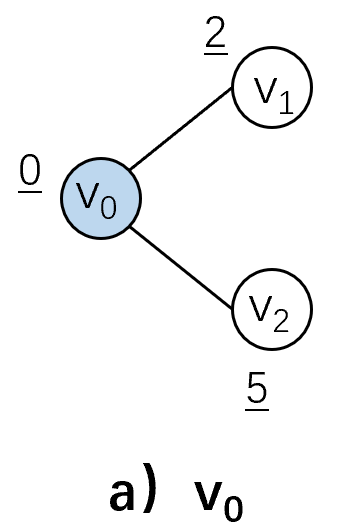
\includegraphics[width=0.67\linewidth]
        {assets/pics_and_ppts/ch5/16迪杰斯特拉过程a.png}
    \end{minipage}

    \item 
    \begin{minipage}[t]{0.65\linewidth}
        \vspace{0pt}
        从未求解顶点集合\{1,2,3,4,5\}中选择$cur\_mind[]$最小的顶点$v_1$，将该顶点的全局最短路径确定为2，并标记$v_1$的Solved[1]为true。然后
        以$v_1$为中介，$v_1$的邻接点有$v_2$、$v_3$、$v_4$，于是分别计算：$cur\_mind[v_1] + cost(v_1, v_2) = 3 < cur\_mind[v_2] = 5$，于是将
        $cur\_mind[v_2]$更新为3；$cur\_mind[v_1] + cost(v_1, v_3) = 12 < cur\_mind[v_3] = +inf$，于是将$cur\_mind[v_3]$更新为12，类似地，
        将$cur\_mind[v_4]$更新为5。并且$v_2$、$v_3$、$v_4$此时都是由$v_1$更新来的，因此将Pre[2]、Pre[3]、Pre[4]记为1。

        如图b）及表\ref{table:迪杰斯特拉算法过程演示}步骤2所示。
    \end{minipage}
    \hfill
    \begin{minipage}[t]{0.30\linewidth}
        \vspace{0pt}
        \centering
        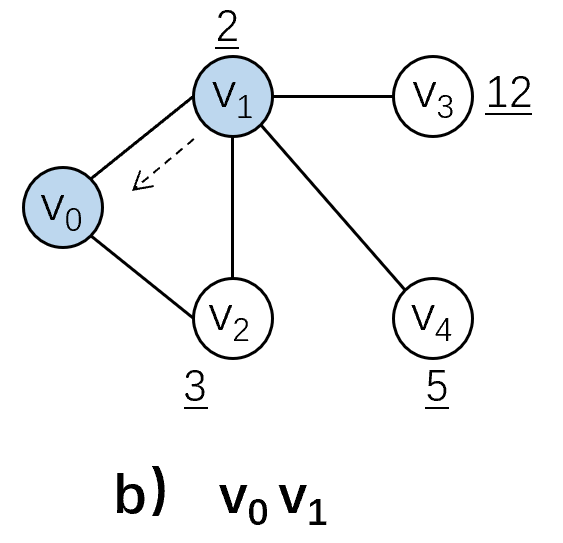
\includegraphics[width=0.88\linewidth]
        {assets/pics_and_ppts/ch5/17迪杰斯特拉过程b.png}
    \end{minipage}

    \item 
    \begin{minipage}[t]{0.65\linewidth}
        \vspace{0pt}
        从未求解顶点集合\{2,3,4,5\}中选择$cur\_mind[]$最小的顶点$v_2$，将Solved[2]标记为true，然后尝试更新$v_4$的$cur\_mind[4]$，但由于
        $cur\_mind[2] + cost(v_2, v_4) = 3 + 8 = 11 > cur\_mind[4] = 5$，因此无需更新。

        这一步其实只将顶点$v_2$标记为了“已求解”，如图c）及表\ref{table:迪杰斯特拉算法过程演示}步骤3所示。

    \end{minipage}
    \hfill
    \begin{minipage}[t]{0.30\linewidth}
        \vspace{0pt}
        \centering
        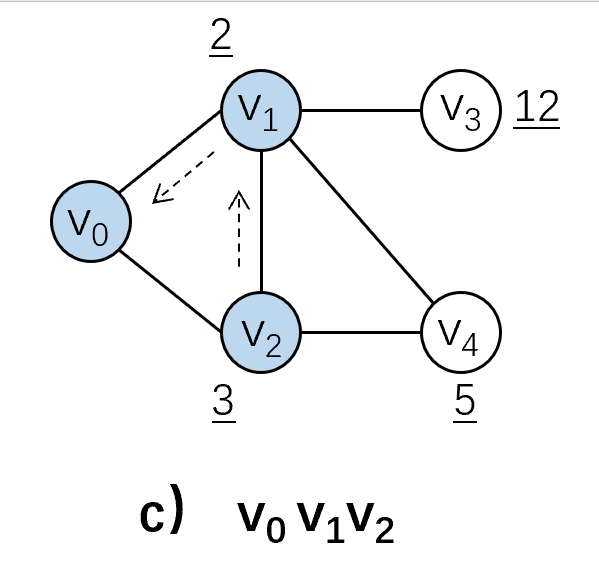
\includegraphics[width=0.90\linewidth]
        {assets/pics_and_ppts/ch5/18迪杰斯特拉过程c.png}
    \end{minipage}

    \item 
    \begin{minipage}[t]{0.65\linewidth}
        \vspace{0pt}
        从\{3,4,5\}中，选择顶点$v_4$，标记Solved[4]为true。并以$v_4$为中介，将$cur\_mind[3]$更新为9、Pre[3]更新为4；将$cur\_mind[5]$更新为5+9=14，将Pre[5]更新为4。

        如图d）及表\ref{table:迪杰斯特拉算法过程演示}步骤4所示。

    \end{minipage}
    \hfill
    \begin{minipage}[t]{0.30\linewidth}
        \vspace{0pt}
        \centering
        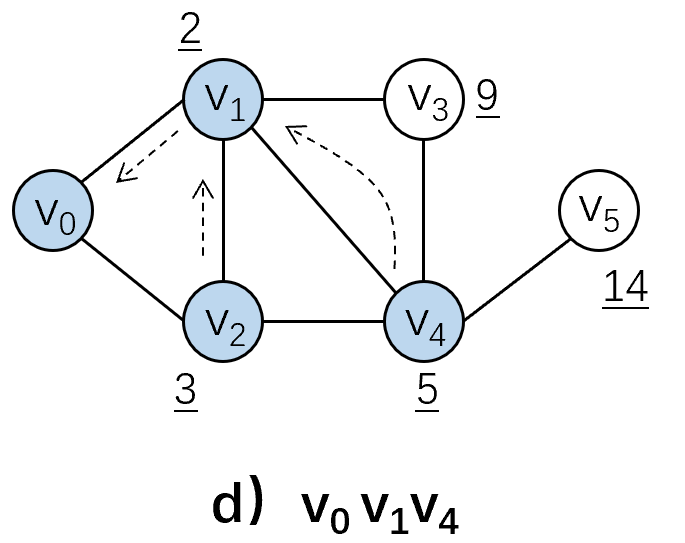
\includegraphics[width=0.99\linewidth]
        {assets/pics_and_ppts/ch5/19迪杰斯特拉过程d.png}
    \end{minipage}

    \item 
    \begin{minipage}[t]{0.65\linewidth}
        \vspace{0pt}
        从\{3,5\}中，选择顶点$v_3$，标记Solved[3]为true。以$v_3$为中介，发现$cur\_mind[3] + cost(3, 5) = 9+6 = 15 > cur\_mind[5] = 14$，因此无需更新。
        此时最后一个顶点$v_5$的最短路径显然也已经确定了，为14。

        如图e）及表\ref{table:迪杰斯特拉算法过程演示}步骤5所示。最后，我们将
        $v_5$标记为已求解顶点即可。

    \end{minipage}
    \hfill
    \begin{minipage}[t]{0.30\linewidth}
        \vspace{0pt}
        \centering
        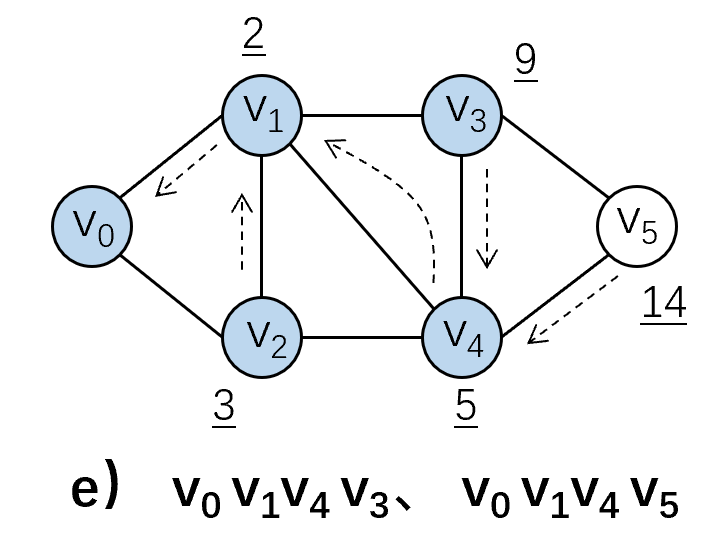
\includegraphics[width=0.99\linewidth]
        {assets/pics_and_ppts/ch5/20迪杰斯特拉过程e.png}
    \end{minipage}

    \item 将最后的顶点$v_5$标记为已求解。如表\ref{table:迪杰斯特拉算法过程演示}步骤6所示。

\end{enumerate}





\begin{table}[htbp]
    \centering
    \caption{迪杰斯特拉算法过程演示}
    \small
    \sffamily
    

    {
    \renewcommand{\arraystretch}{1.6}
    \setlength{\tabcolsep}{5pt}
    \setlength{\arrayrulewidth}{0.8pt}
    \arrayrulecolor{white}

    \begin{tabular}{
        |>{\columncolor{stepbg}\centering\arraybackslash}m{1.15cm}
        |>{\columncolor{fieldbg}\raggedright\arraybackslash}m{1.6cm}
        |*{7}{>{\columncolor{datablue}\color{white}\centering\arraybackslash}m{1.25cm}|}
    }
        \hline

        % 表头
        \multicolumn{2}{|c|}{
            \cellcolor{headblue}
            {\color{white}
            \diagbox[width=3.2cm,height=1.15cm,dir=NW]
            {\bfseries 步骤}
            {\bfseries 顶点}}
        }
        & \cellcolor{headblue}\textbf{0}
        & \cellcolor{headblue}\textbf{1}
        & \cellcolor{headblue}\textbf{2}
        & \cellcolor{headblue}\textbf{3}
        & \cellcolor{headblue}\textbf{4}
        & \cellcolor{headblue}\textbf{5}
        & \cellcolor{headblue}\textbf{剩余未求解顶点集合}
        \\
        \hline

        % 初始状态
        初始
        & \shortstack[l]{cur\_mind[]\\Pre[]\\Solved[]}
        & \shortstack[l]{0\\[0.23em]-1\\[0.23em]false} & \shortstack[l]{+inf\\[0.23em]-1\\[0.23em]false} & \shortstack[l]{+inf\\[0.23em]-1\\[0.23em]false} 
            & \shortstack[l]{+inf\\[0.23em]-1\\[0.23em]false}
        & \shortstack[l]{+inf\\[0.23em]-1\\[0.23em]false} & \shortstack[l]{+inf\\[0.23em]-1\\[0.23em]false} & \shortstack[l]{\{0,1,2,\\3,4,5\}}
        \\
        \hline

        % 第 1 步
        1
        & \shortstack[l]{cur\_mind[]\\Pre[]\\Solved[]}
        & \shortstack[l]{0\\[0.23em]-1\\[0.23em]\textbf{true}} & \shortstack[l]{\textbf{2}\\[0.23em]\textbf{0}\\[0.23em]false} & \shortstack[l]{\textbf{5}\\[0.23em]\textbf{0}\\[0.23em]false} 
            & \shortstack[l]{+inf\\[0.23em]-1\\[0.23em]false}
        & \shortstack[l]{+inf\\[0.23em]-1\\[0.23em]false} & \shortstack[l]{+inf\\[0.23em]-1\\[0.23em]false} & \shortstack[l]{\{1,2,\\3,4,5\}}
        \\
        \hline

        % 第 2 步
        2
        & \shortstack[l]{cur\_mind[]\\Pre[]\\Solved[]}
        & \shortstack[l]{0\\[0.23em]-1\\[0.23em]true} & \shortstack[l]{2\\[0.23em]0\\[0.23em]\textbf{true}} & \shortstack[l]{\textbf{3}\\[0.23em]\textbf{1}\\[0.23em]false} 
            & \shortstack[l]{\textbf{12}\\[0.23em]\textbf{1}\\[0.23em]false}
        & \shortstack[l]{\textbf{5}\\[0.23em]\textbf{1}\\[0.23em]false} & \shortstack[l]{+inf\\[0.23em]-1\\[0.23em]false} & \{2,3,4,5\}
        \\
        \hline

        % 第 3 步
        3
        & \shortstack[l]{cur\_mind[]\\Pre[]\\Solved[]}
        & \shortstack[l]{0\\[0.23em]-1\\[0.23em]true} & \shortstack[l]{2\\[0.23em]0\\[0.23em]true} & \shortstack[l]{3\\[0.23em]1\\[0.23em]\textbf{true}} 
            & \shortstack[l]{12\\[0.23em]1\\[0.23em]false}
        & \shortstack[l]{5\\[0.23em]1\\[0.23em]false} & \shortstack[l]{+inf\\[0.23em]-1\\[0.23em]false} & \{3,4,5\}
        \\
        \hline

        % 第 4 步
        4
        & \shortstack[l]{cur\_mind[]\\Pre[]\\Solved[]}
        & \shortstack[l]{0\\[0.23em]-1\\[0.23em]true} & \shortstack[l]{2\\[0.23em]0\\[0.23em]true} & \shortstack[l]{3\\[0.23em]1\\[0.23em]true} 
            & \shortstack[l]{\textbf{9}\\[0.23em]\textbf{4}\\[0.23em]false}
        & \shortstack[l]{5\\[0.23em]1\\[0.23em]\textbf{true}} & \shortstack[l]{\textbf{14}\\[0.23em]\textbf{4}\\[0.23em]false} & \{3,5\}
        \\
        \hline

        % 第 5 步
        5
        & \shortstack[l]{cur\_mind[]\\Pre[]\\Solved[]}
        & \shortstack[l]{0\\[0.23em]-1\\[0.23em]true} & \shortstack[l]{2\\[0.23em]0\\[0.23em]true} & \shortstack[l]{3\\[0.23em]1\\[0.23em]true} 
            & \shortstack[l]{9\\[0.23em]4\\[0.23em]\textbf{true}}
        & \shortstack[l]{5\\[0.23em]1\\[0.23em]true} & \shortstack[l]{14\\[0.23em]4\\[0.23em]false} & \{5\}
        \\
        \hline

        % 第 6 步
        6
        & \shortstack[l]{cur\_mind[]\\Pre[]\\Solved[]}
        & \shortstack[l]{0\\[0.23em]-1\\[0.23em]true} & \shortstack[l]{2\\[0.23em]0\\[0.23em]true} & \shortstack[l]{3\\[0.23em]1\\[0.23em]true} 
            & \shortstack[l]{9\\[0.23em]4\\[0.23em]true}
        & \shortstack[l]{5\\[0.23em]1\\[0.23em]true} & \shortstack[l]{14\\[0.23em]4\\[0.23em]\textbf{true}} & \{\;\}
        \\
        \hline

    \end{tabular}
    }
    \label{table:迪杰斯特拉算法过程演示}
\end{table}

% 恢复表格样式
\arrayrulecolor{black}
\setlength{\arrayrulewidth}{0.5pt}

可以看到，“选点”就是每次从尚未求解的集合中，“选”出一个当前已知最短路径$cur\_mind[]$最小的顶点v，作为“已求解顶点”，并用它尝试“更新”其所有邻接点的
最短路径$cur\_mind[]$。每次能确定一个顶点的全局最短路径，重复$N$次操作（其实$N-1$次即可），即可求解所有顶点的全局最短路径，最终$cur\_mind[]$
中保存的就是各个顶点的全局最短路径的长度，而各顶点的最短路径是什么，顺着Pre[]数组一路向前即可。如$v_5$到$v_0$的最短路径就是
\begin{bulk}
    5 -> Pre[5] = 4 -> Pre[4] = 1 -> Pre[1] = 0，即 5 -> 4 -> 1 -> 0    
\end{bulk}
这就是赫赫有名的迪杰斯特拉算法。迪杰斯特拉算法可以求解出从源点s到各个与之连通的顶点之间的最短路径，同时也可以确定哪些顶点与s是不连通的。但迪杰斯特拉算法要求
图中不存在从源点出发可达的负权边，\textbf{若图不满足这一条件，迪杰斯特拉算法将失效}。

迪杰斯特拉算法需要$N$次“选点”、“更新”操作，更新时需要找到该顶点的所有邻接点，而对于邻接矩阵和邻接表存储的图，找邻接点的时间复杂度有所区别，因此，迪杰斯特拉
算法的时间复杂度与图的存储方式有关，下面我们就看看两种存储方式下，迪杰斯特拉算法如何实现。

\minisection{1.迪杰斯特拉算法实现（邻接矩阵版）}
有了前面的思路，我们可以很轻松地写出迪杰斯特拉算法的代码。唯一需要注意的就是需要正确处理图中存在顶点不可达的情况，详请参见如下代码及注释。

\begin{cppcode}
    int Matrix[N][N];   // 邻接矩阵，存放边权，若边不存在用-1表示
    bool Solved[N];     // 已初始化为false
    int Pre[N];         // 已初始化为-1
    int cur_mind[N];    // 已初始化为 +inf。
    const int inf = 0x3fffffff; // +inf
    // 求解以s为源点的单源最短路径
    void Dijkstra(int s) {
        cur_mind[s] = 0;
        // 该层循环用于执行N次“选点”、“更新”的操作
        for(int i=0; i<N; i++) {
            // 选出未求解的顶点中，cur_mind[]最小的顶点v
            int min_cur_mind = inf;
            int v = -1;
            for(int j=0; j<N; j++) {
                if(Solved[j] == false && cur_mind[j] < min_cur_mind) {
                    min_cur_mind = cur_mind[j];
                    v = j;
                }
            }

            /* 这里是为了处理图中存在顶点不可达的情况。
             若存在顶点不可达，则将可达顶点全选完之后，
             接下来一定会“选不到顶点”，所以若没选到顶点，
             则v的值是无意义的，不应执行后面的代码。*/
            if(v == -1) {
                break;
            }
            
            Solved[v] = true;
            // 以v为中介，尝试更新其所有邻接点
            for(int u=0; u<N; u++) {
                // v到u有路径并且u的全局最短还未确定 不判断Solved[u] == false性能稍差一点，但影响不大。
                if(Matrix[v][u] != -1 && Solved[u] == false) {    
                    if(cur_mind[v] + Matrix[v][u] < cur_mind[u]) {
                        cur_mind[u] = cur_mind[v] + Matrix[v][u];
                        Pre[u] = v;
                    }
                }
            } 
        } 
    }
    
\end{cppcode}
对于以上邻接矩阵版的代码，需要$N$次“选点”、“更新”操作，外层循环时间为$O(N)$，每次选点时遍历一遍cur\_mind[]数组的时间是$O(N)$，更新时需要找到该顶点的所有邻接点，
时间是$O(N)$，整体的时间复杂度为$O(N^2)$。空间方面，需要额外引入Pre[]、Solved[]、cur\_mind[]三个数组，空间复杂度为$O(N)$。

注意：邻接矩阵是存储图本身所需要的空间，不属于迪杰斯特拉算法带来的空间开销，不能算在算法的空间复杂度中。

\minisection{2.迪杰斯特拉算法实现（邻接表版）}
邻接表版仅在获取顶点的邻接点信息时代码有所不同。邻接表版代码如下所示。
\begin{cppcodeHighlight}[1-5,30-36]
    struct AdjEdge {
        int u;      // 邻接点的编号
        int weight; // 边权
    };
    vector<AdjEdge> AdjList[N];    // 邻接表
    bool Solved[N];     // 已初始化为false
    int Pre[N];         // 已初始化为-1
    int cur_mind[N];    // 已初始化为 +inf。
    const int inf = 0x3fffffff; // +inf
    // 求解以s为源点的单源最短路径
    void Dijkstra(int s) {
        cur_mind[s] = 0;
        for(int i=0; i<N; i++) {
            // 选出未求解的顶点中，cur_mind[]最小的顶点v
            int min_cur_mind = inf;
            int v = -1;
            for(int j=0; j<N; j++) {
                if(Solved[j] == false && cur_mind[j] < min_cur_mind) {
                    min_cur_mind = cur_mind[j];
                    v = j;
                }
            }

            if(v == -1) {
                break;
            }
            
            Solved[v] = true;
            // 以v为中介，尝试更新其所有邻接点
            for(int j=0; j<AdjList[v].size(); j++) {
                int u = AdjList[v][j].u;  // 与v邻接的顶点u
                if(cur_mind[v] + AdjList[v][j].weight < cur_mind[u]) {
                    cur_mind[u] = cur_mind[v] + AdjList[v][j].weight;
                    Pre[u] = v;
                }
            }
        } 
    }
\end{cppcodeHighlight}
对于以上邻接表版的代码，外层循环时间同样为$O(N)$，每次选点时遍历一遍cur\_mind[]数组的时间同样是$O(N)$，而更新时找到该顶点的所有邻接点的操作
实际上与外层循环无关，是对整个图来说需要进行约$M$次，$M$为图的边数。因此邻接表版时间复杂度为$O(N^2+M)$。

空间方面，与邻接矩阵版本类似，同样是需要额外引入Pre[]、Solved[]、cur\_mind[]三个数组，空间复杂度为$O(N)$。

请注意，上面的代码中，每次寻找当前cur\_mind[]最小的顶点时，我们是遍历一遍数组，为O(N)的时间。事实上，可以使用前面介绍过的数据结构---\textbf{堆}
（C++中的priority\_queue）来完成，每次以O(1)时间
即可返回最小的元素。若图采用邻接表实现，这种堆优化的迪杰斯特拉算法的\textbf{最坏}时间复杂度可以达到$O((N+M)logN)$。由于priority\_queue在此处的使用涉及
稍复杂的C++原理，因此不在此处给出代码，感兴趣的同学可以自己尝试写出。



\subsection{Bellman-Ford算法}
几乎在迪杰斯特拉算法诞生的同期，也诞生了另外一个求解单源最短路径的算法：Bellman-Ford 算法。它与 Dijkstra 算法有一个重要区别：只要从源
点出发能够到达的范围内不存在负权\uline{环}，Bellman-Ford 算法就能够正确求得单源最短路径，即使图中存在负权边也没有问题。\\

Bellman-Ford算法的核心思想是：反复对图中的\uline{所有边}进行松弛操作。具体来说，假设图中有$N$个顶点$M$条边，源点为s，与迪杰斯特拉算法类似，定义：
cur\_mind[v]为当前已知的从s到v的最短路径长度，初始化cur\_mind[s]为0，其他顶点的cur\_mind[]均为正无穷。

然后，对图中的每一条边$(u, v)$ 进行松弛操作：
\[
    dist[v]=\min(dist[v], dist[u] + cost(u,v))
\]
其中，\(cost(u,v)\) 表示边 \((u,v)\) 的权值（路径长度）。对所有边完成一轮松弛后，再进行下一轮，则最多进行 \(N-1\) 轮后，所有顶点的cur\_mind[]就已经是
全局最短路径。

为什么这个算法是正确的？

如图\ref{fig:BellmanFord算法理解}所示，以$v_2$为起点，$v_1$到$v_2$的最短路径是1条边的路径：$v1 -> v2$，因此第一轮操作之后就能考虑到，并将其长度1赋值给
cur\_mind[1]，此后无论如何cur\_mind[1]也不会再被更新。
\begin{figure}[htbp]
    \centering
    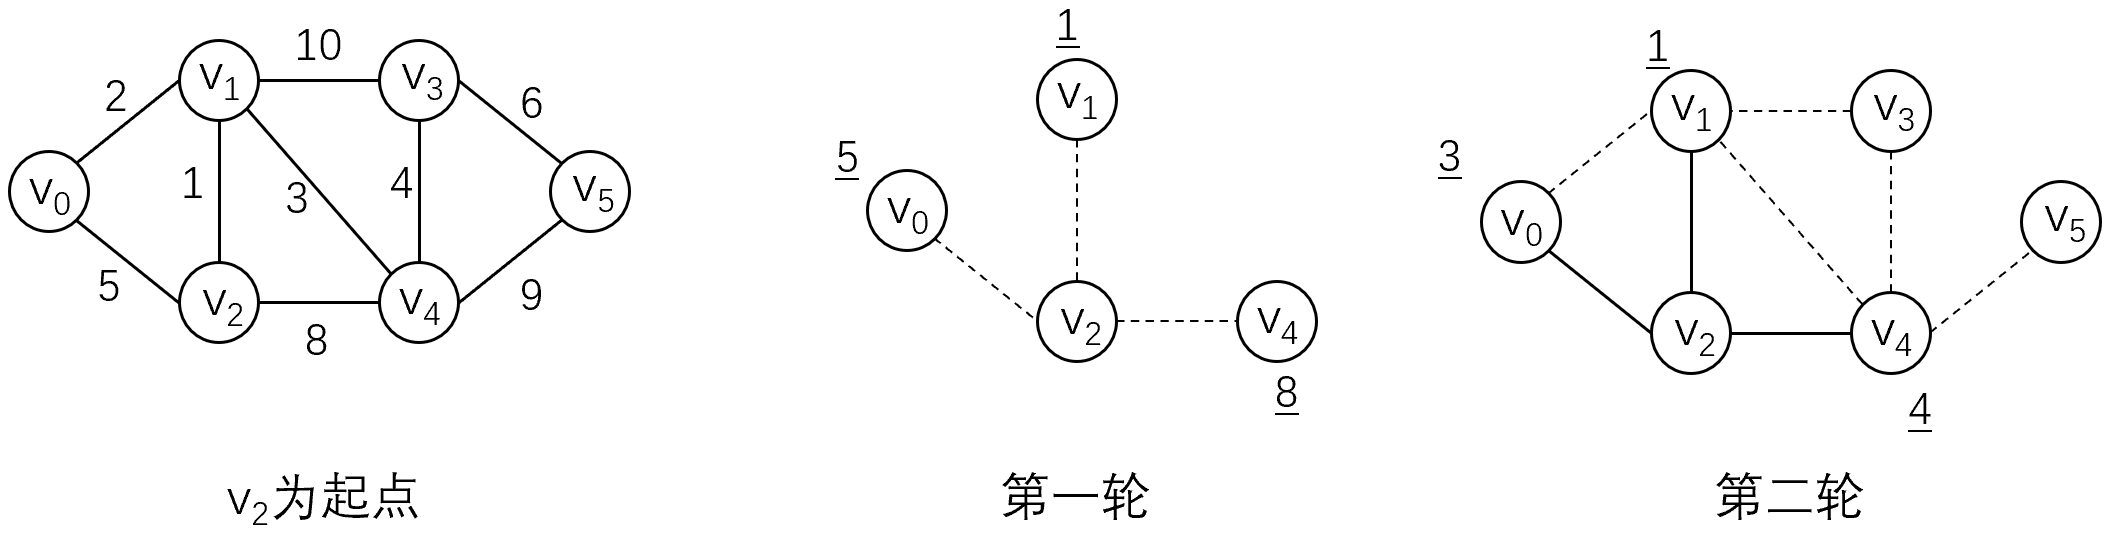
\includegraphics[width=0.85\textwidth]{assets/pics_and_ppts/ch5/22BellmanFord算法理解.png}
    \caption{}
    \label{fig:BellmanFord算法理解}
\end{figure}

$v_0$到$v_2$的最短
路径是$v_0 -> v_1 -> v_2$、$v_4$到$v_2$的最短路径是$v_4 -> v_1 -> v_2$，都是2条边的最短路径，因此第二轮操作之后就能考虑到这些路径，并且赋值给
cur\_mind[0]、cur\_mind[4]，之后绝对不会再改变。

Bellman-Ford 算法每完成一轮对所有边的松弛，就能够保证考虑到最多多一条边的路径，因此$N-1$轮之后，就能考虑到最多$N-1$条边的路径。而
如果源点可达范围不存在负权环，那么任意两个顶点之间的最短路径一定不包含重复顶点，路径最多$N-1$条边。

此外，如果完成 \(N-1\) 轮后，再对所有边进行一轮松弛，仍然能够更新某个顶点的距离，就说明存在从源点可达的负权环。若图存在从源点可达的负环，则显然在负环
中不断转圈可以让最短路径无限地小下去，直至负无穷。因此，通过以上手段Bellman-Ford算法可以在图不存在负环时给出正确解，并在图存在负环时给出“问题不可解”的结论。

Bellman-Ford 算法需要做约$N$轮操作，每轮操作需要遍历所有边，对于邻接矩阵存储的图，遍历所有边需要遍历邻接矩阵，时间为$O(N^2)$，而对于邻接表，遍历所有边
需要遍历邻接表，时间为$O(M)$。因此对于邻接矩阵存储的图，Bellman-Ford时间复杂度为$O(N^3)$，对于邻接表存储的图，Bellman-Ford的时间复杂度为$O(NM)$。

对于邻接表存储的图，Bellman-Ford算法的实现如下所示：
\begin{cppcode}
    struct AdjEdge {
        int u;
        int weight;
    };
    vector<AdjEdge> AdjList[N]; // 已存储图的邻接表
    const int inf = 0x3fffffff;
    int cur_mind[N];    // 已初始化为inf
    int Pre[N];     // 已初始化为-1
    bool BellmanFord(int s) {
        cur_mind[s] = 0;
        // 做N-1次
        for(int i=0; i<N-1; i++) {
            // 遍历所有边
            for(int v=0; v<N; v++) {
                // 与v邻接的所有边
                for(int k=0; k<AdjList[v].size(); k++) {
                    int u = AdjList[v][k].u;
                    int weight = AdjList[v][k].weight;
                    if(cur_mind[v] + weight < cur_mind[u]) {
                        cur_mind[u] = cur_mind[v] + weight;
                        Pre[u] = v;
                    }

                }
            }
        }

        // 再做一次，判断是否存在负环
        for(int v=0; v<N; v++) {
            for(int k=0; k<AdjList[v].size(); k++) {
                int u = AdjList[v][k].u;
                int weight = AdjList[v][k].weight;
                if(cur_mind[v] + weight < cur_mind[u]) {
                    return false;
                }

            }
        }
        return true;
    }
\end{cppcode}
当图存在负环时，Bellman-Ford算法返回false，表示存在负环，最短路径问题不可解。否则返回true，cur\_mind[]数组中存放的就是各顶点的最短路径。沿着Pre[]数组
往回追溯即可得到轨迹。对于邻接矩阵版本仅在于遍历边的方式不同，这里不再给出代码。

可以看到，与Dijkstra算法从源点出发，逐渐向外“扩散”地求解各个顶点的最短路径的策略不同，Bellman-Ford算法则是“放眼全局”，一步一步地让全局下的各个cur\_mind[]
慢慢向正确解“收拢”。\\

对于Bellman-Ford算法，我们自然会想到这样一个问题：我们每轮处理的时候，都需要遍历所有边，判断能否更新某个顶点的cur\_mind[]。但事实上，假设第$i-1$轮
仅有顶点v的cur\_mind[]发生了变化，那么第$i$轮其实我们没有必要遍历所有边，而是只遍历v的出边即可，因为只有距离发生了变化的顶点才可能继续影响其他顶点。这样，
仅处理距离发生了变化的边，就大大提高了算法的效率。因此对于上面的代码，在以下条件成立时：
\begin{cppcode}
    if(cur_mind[v] + weight < cur_mind[u]) {
        cur_mind[u] = cur_mind[v] + weight;
        Pre[u] = v;
    }
\end{cppcode}
说明u是一个距离发生了变化的顶点，我们将其放入队列中。

于是思路就是：最初将起点s放入队列，并在每次处理时，将那些距离发生了改变的顶点入队。当队列为空时，说明没有新的顶点距离发生改变，也就处理完了。但是这样做有两个新的问题：

（1）反复入队问题。

\begin{wrapfigure}{r}{0.27\textwidth}
    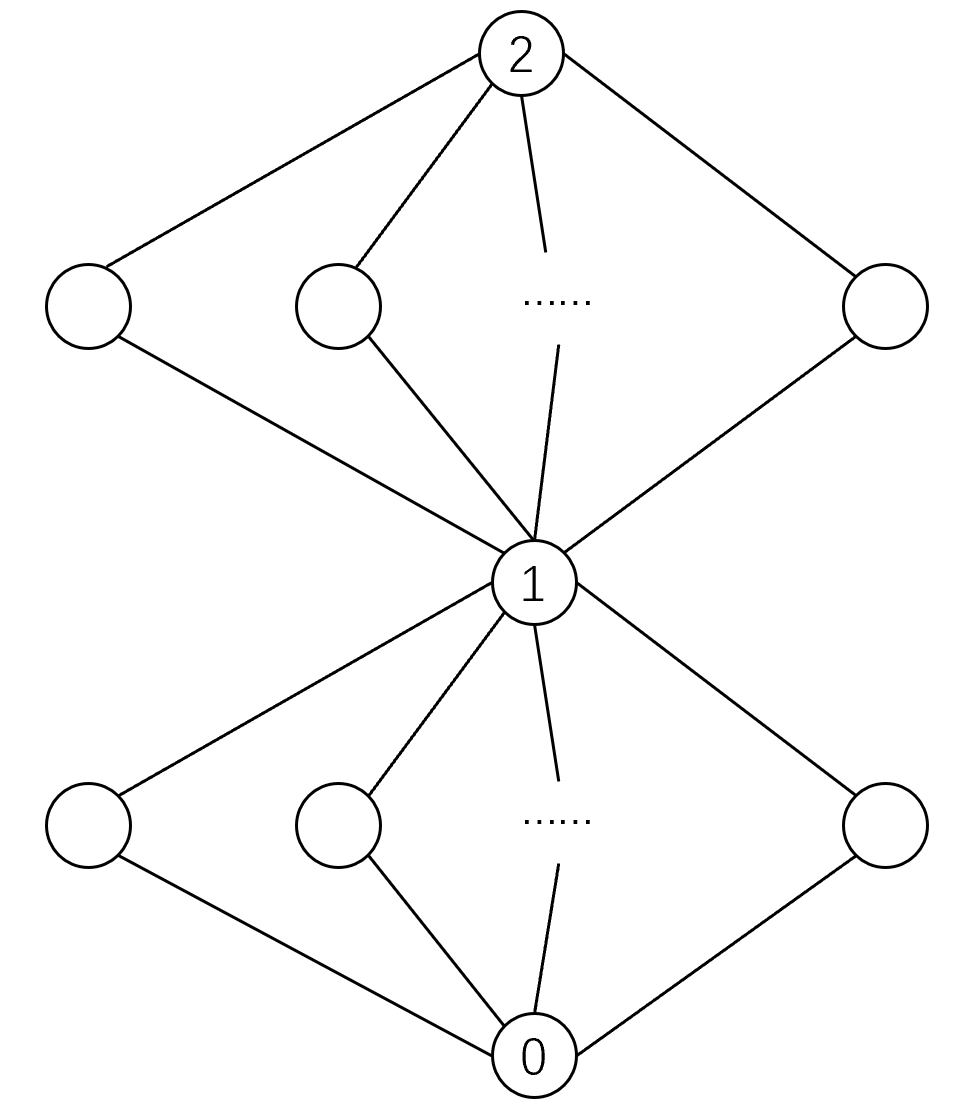
\includegraphics[width=0.35\textwidth]{assets/pics_and_ppts/ch5/23SPFA反复入队导致性能雪崩.png}
    \caption{反复入队问题}
    \label{fig:SPFA反复入队导致性能雪崩}
\end{wrapfigure}

如图\ref{fig:SPFA反复入队导致性能雪崩}所示，假设0为起点，向上松弛的若干顶点，将这些顶点入队后，
取出时，对每一个顶点的处理都可能将顶点1松弛一遍，如果每次都将1入队就造成了重复入队，会出现很多无意义的重复处理，继续向外传导，会造成指数级的性能灾难。因此要
解决这个问题，就需要引入一个数组in\_queue[N]，标识每一个顶点是否已经在队列中了，顶点此时不在队列中时才将它入队。



（2）负环判断问题。这种做法一直做到队列为空，若存在负环，则永远会有新的顶点距离变小，队列永远不会空。那怎么办？常见的做法是再记录一个数组
inq\_cnt[N]，标记每个顶点入队的次数。若某个顶点已经入队了超过$N-1$次（它的距离已经被更新过超过$N-1$次），说明存在负环，问题不可解。

于是我们可以给出这种优化的Bellman-Ford算法代码（邻接表版）如下所示：
\begin{cppcode}
    struct AdjEdge {
        int u;
        int weight;
    };
    vector<AdjEdge> AdjList[N]; // 已存储图的邻接表
    const int inf = 0x3fffffff;
    int cur_mind[N];    // 已初始化为inf
    int Pre[N];     // 已初始化为-1

    bool in_queue[N];   // 标记顶点是否当前在队列中，初始化为false
    int inq_cnt[N];         // 记录顶点入队次数，用于检测负权环，初始化为0
    bool SPFA(int s) {
        cur_mind[s] = 0;
        queue<int> q;
        q.push(s);
        in_queue[s] = true;

        while(!q.empty()) {
            int v = q.front();
            q.pop();
            
            // 弹出后，别忘了将标记改为 false，允许它以后再次入队
            in_queue[v] = false;

            // 遍历当前顶点的所有出边
            for(int j = 0; j < AdjList[v].size(); j++) {
                int u = AdjList[v][j].u;
                int weight = AdjList[v][j].weight;

                // 松弛操作
                if(cur_mind[v] + weight < cur_mind[u]) {
                    cur_mind[u] = cur_mind[v] + weight;
                    Pre[u] = v;

                    // 如果 u 不在队列中，将其压入队列
                    if(!in_queue[u]) {
                        q.push(u);
                        in_queue[u] = true;
                        inq_cnt[u]++; // 记录入队次数

                        // 如果某个顶点入队次数超过 N-1 次，说明存在负权环
                        if(inq_cnt[u] >= N) {
                            return false; 
                        }
                    }
                }
            }
        }

        return true; 
    }
\end{cppcode}

这种优化后的Bellman-Ford算法被称为\term{SPFA（Shortest Path Faster Algorithm）算法}。它的平均时间复杂度为O(kM)，k是每个顶点的
平均入队次数，而最坏时间复杂度为O(NM)。在大多数场景下SPFA算法性能要由于堆优化后的迪杰斯特拉算法，但对于极端情况，迪杰斯特拉算法
最差也能保证O((N+M)logN)的复杂度，而SPFA算法可能达到O(NM)。


\subsection{Floyd算法}
Floyd 算法（弗洛伊德算法），是一种用于求解图中所有顶点对之间最短路径的算法，即\term{全源最短路径}问题。。
Floyd算法的核心思想在于：对于任意三个顶点 \(i\)、\(j\)、\(k\)，我们都可以尝试：
\[
    d_{ij}=\min(d_{ij},d_{ik}+d_{kj})
\]
也就是说，我们原来知道的\(i\) 到 \(j\) 的最短距离是 \(d_{ij}\)，现在尝试让路径经过顶点 \(k\)，如果经过 \(k\) 的距离更短，就更新答案。

顶点到自身的距离初始化为$0$，存在直接边的顶点之间距离初始化为边权，不存在直接边的顶点之间距离初始化为正无穷。算法实现如下：
\begin{cppcode}
    const int inf = 0x3fffffff;
    int d[N][N];

    // 初始化距离矩阵
    for (int i = 0; i < N; i++) {
        for (int j = 0; j < N; j++) {
            d[i][j] = (i == j ? 0 : inf);
        }
    }

    // 根据图中的边更新距离矩阵
    // 假设存在一条从u到v、权重为w的边
    degree[u][v] = w;
    // ...

    // Floyd算法
    for (int k = 0; k < N; k++) {
        for (int i = 0; i < N; i++) {
            for (int j = 0; j < N; j++) {
                if (d[i][k] != inf &&
                    d[k][j] != inf) {
                    d[i][j] = min(
                        d[i][j],
                        d[i][k] + d[k][j]
                    );
                }
            }
        }
    }
\end{cppcode}
Floyd算法支持存在负权边的图，但要求不存在从源点可达的负权环。其时间复杂度为$O(N^3)$，空间复杂度为$O(N^2)$。






\chapter*{--- BONFIRE ENCOUNTERED ---}%%%%%%%%%%%%%%%%%%%%%%%%%%%%%%%%%%%%%%%%%%%%%%%%%%%%%%%%%%%%%%%%%%%%%%%%%%%%%%%%%%%%%%%%%%%%%%%%%%%%%%%%%%%%%%%%%%%%%%%%%%%%%%%%%%%%%%%%%%
火光闪烁中，你独自坐在营火旁。


\begin{exercise}
1. （某年408真题）使用迪杰斯特拉算法求下图中顶点1到其他各顶点之间的最短路径，则依次确定最短路径的目标定点是\underline{\hspace{1cm}}
\begin{center}
    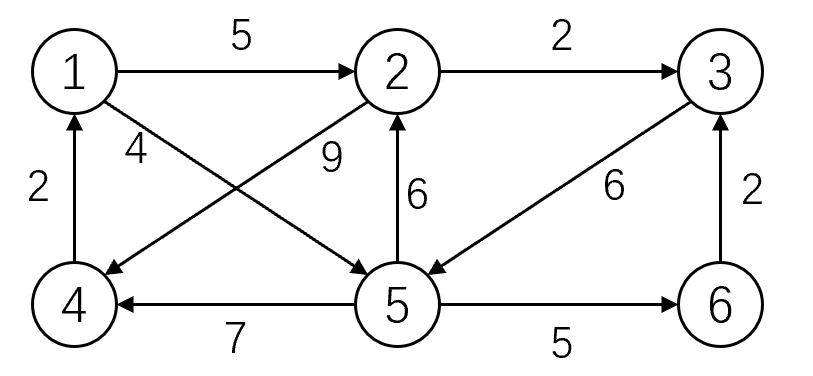
\includegraphics[width=0.40\textwidth]{assets/pics_and_ppts/ch5/习题09，16408最短路径的选点顺序.png}
\end{center}

\begin{tabular}{llll}
    A. 5,2,3,4,6 & B. 5,2,3,6,4 & C. 5,2,4,3,6 & D. 5,2,6,3,4
\end{tabular}

\vspace{\baselineskip}

2. （某年408真题）对下图所示的有向带权图，若采用迪杰斯特拉算法求源点a到其他各顶点的最短路径，则第一个确定全局最短路径的顶点是b，第二个确定全局最短路径
的顶点是c，后续的顶点依次是\underline{\hspace{1cm}}

\begin{center}
    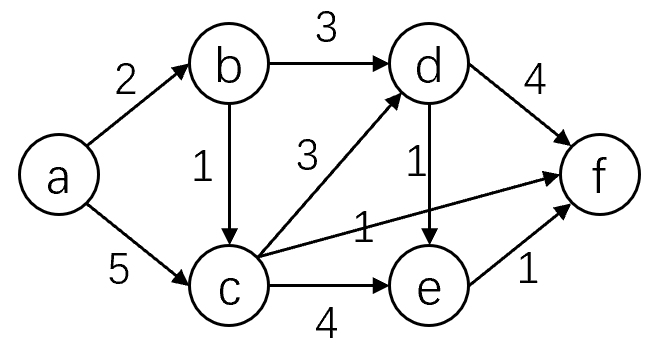
\includegraphics[width=0.34\textwidth]{assets/pics_and_ppts/ch5/习题10，12408最短路径选点顺序.png}
\end{center}

\begin{tabular}{llll}
    A. d,e,f & B. e,d,f & C. f,d,e & D. f,e,d
\end{tabular}

\vspace{\baselineskip}

3. （某年408真题）使用迪杰斯特拉算法求下图中从顶点1到其余各顶点的最短路径，将当前找到的从顶点1到顶点2，3，4，5的最短路径
保存在数组dist[]中，则依次求出两个顶点（不包括源点1）的最短路径后，dist中的内容更新为\underline{\hspace{1cm}}

\begin{center}
    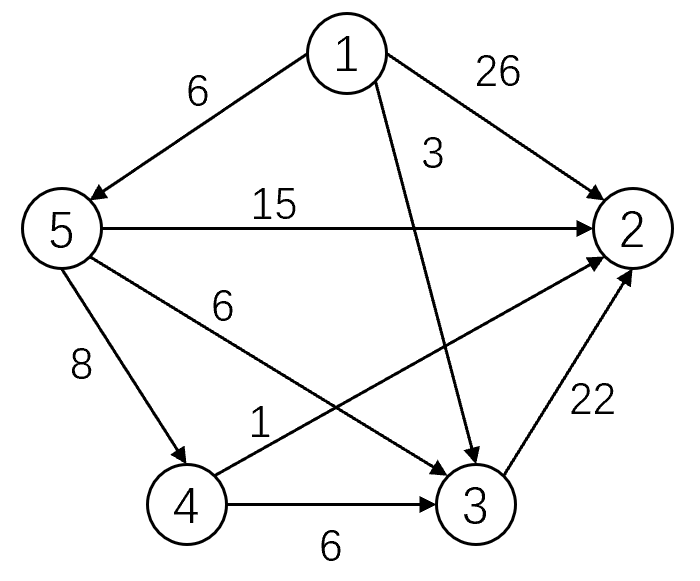
\includegraphics[width=0.33\textwidth]{assets/pics_and_ppts/ch5/习题11，21408迪杰斯特拉dist内容.png}
\end{center}

\begin{tabular}{llll}
    A. 26,3,14,6 & B. 25,3,14,6 & C. 21,3,14,6 & D. 15,3,14,6
\end{tabular}

\vspace{\baselineskip}

4. 请你说明：迪杰斯特拉算法、Bellman-Ford算法以及SPFA算法应对以下情况的图时会怎样？\\[0.5em]
a）存在从源点可达的负环；\\
b）不存在从源点可达的负环，但存在从源点可达的负权边；\\

维火女被邪恶的恶魔、大陆守护神的孪生兄弟LoopCore抓了起来，并关在了监牢的某个牢房里。监牢可以被建模为一个图$G=(V,E)$，顶点表示牢房。

已知该监牢有 $N$ 个牢房，编号为 0 到 $N-1$，牢房之间均存在双向通路，用邻接表存储图模型。你毫不犹豫地动身前往牢房营救维火女，但你破门而入后意外地被魔法传送进了牢房s。\\

5. 已知每个牢房（顶点）的数据类型为char：维火女所在的牢房为\textquotesingle T\textquotesingle，其余牢房均为\textquotesingle F\textquotesingle。
给出在每两个牢房之间移动所需要花费的时间time\_cost（非负），请你计算从s出发，到达维火女的房间所需要的最短时间是多少，若无法到达，返回-1。

\begin{cppcode}
    // N 已定义
    struct AdjEdge {
        int u;          // 顶点编号
        int time_cost;  // 花费时间（边权）
    };
    vector<AdjEdge> AdjList[N];    // 已存储邻接表信息 
    char ver_info[N];   // 已存储顶点信息
    // 返回以s为起点到达维火女的房间需要花费的最短时间
    int MinTime(int s) {
        
    }
\end{cppcode}

\vspace{\baselineskip}

6. 在{\color{red}上题}条件下，假设你在任何两个房间移动时需要和敌人战斗，此时邻接边（AdjEdge）使用如下结构定义：
\begin{cppcode}
    struct AdjEdge {
        int u;              
        int time_cost;      // 花费时间
        int energy_cost;    // 和敌人战斗需要消耗的能量值
    };
\end{cppcode}
保证所有边的time\_cost和energy\_cost均非负。你决定选择所有路线中，消耗时间最少的路线去营救维火女。若有多条路线消耗时间相等，你将选择其中
消耗能量最少的一条路线。

编写一个函数，返回你所选择的路线所消耗的能量值。若无法到达，返回-1。\\

% *7. 在{\color{red}上题}条件下，若你的初始能量值为$e_1$，并且在你到达维火女的房间后，至少还剩有$e_2$的能量值的前提下，才能带她一起离开监牢。
% 现要求你找到她后，必须能够带她离开监牢。在此前提下，你将选择时间最短的一条路线，若有多条路线，你将选择消耗能量最少的路线。请返回在此路线下你
% 到达维火女的房间时剩余的能量值。

% \begin{cppcode}
%     // N 已定义
%     struct AdjEdge {
%         int u;              
%         int time_cost;      // 花费时间
%         int energy_cost;    // 和敌人战斗需要消耗的能量值
%     };
%     vector<AdjEdge> AdjList[N];    // 已存储邻接表信息 
%     char ver_info[N];   // 已存储顶点信息
%     // 返回以s为起点到达维火女的房间需要花费的最短时间
%     int RemainingEnergy(int s, int e1, int e2) {
        
%     }
% \end{cppcode}



\end{exercise}
\clearpage

\begin{exerciseanswer}
1. 选B。每一步所选的点，及选完该点后所有点的当前已知最短路径cur\_mind[]如下图所示（带下划线的数字表示该顶点的cur\_mind[]）。
\begin{center}
    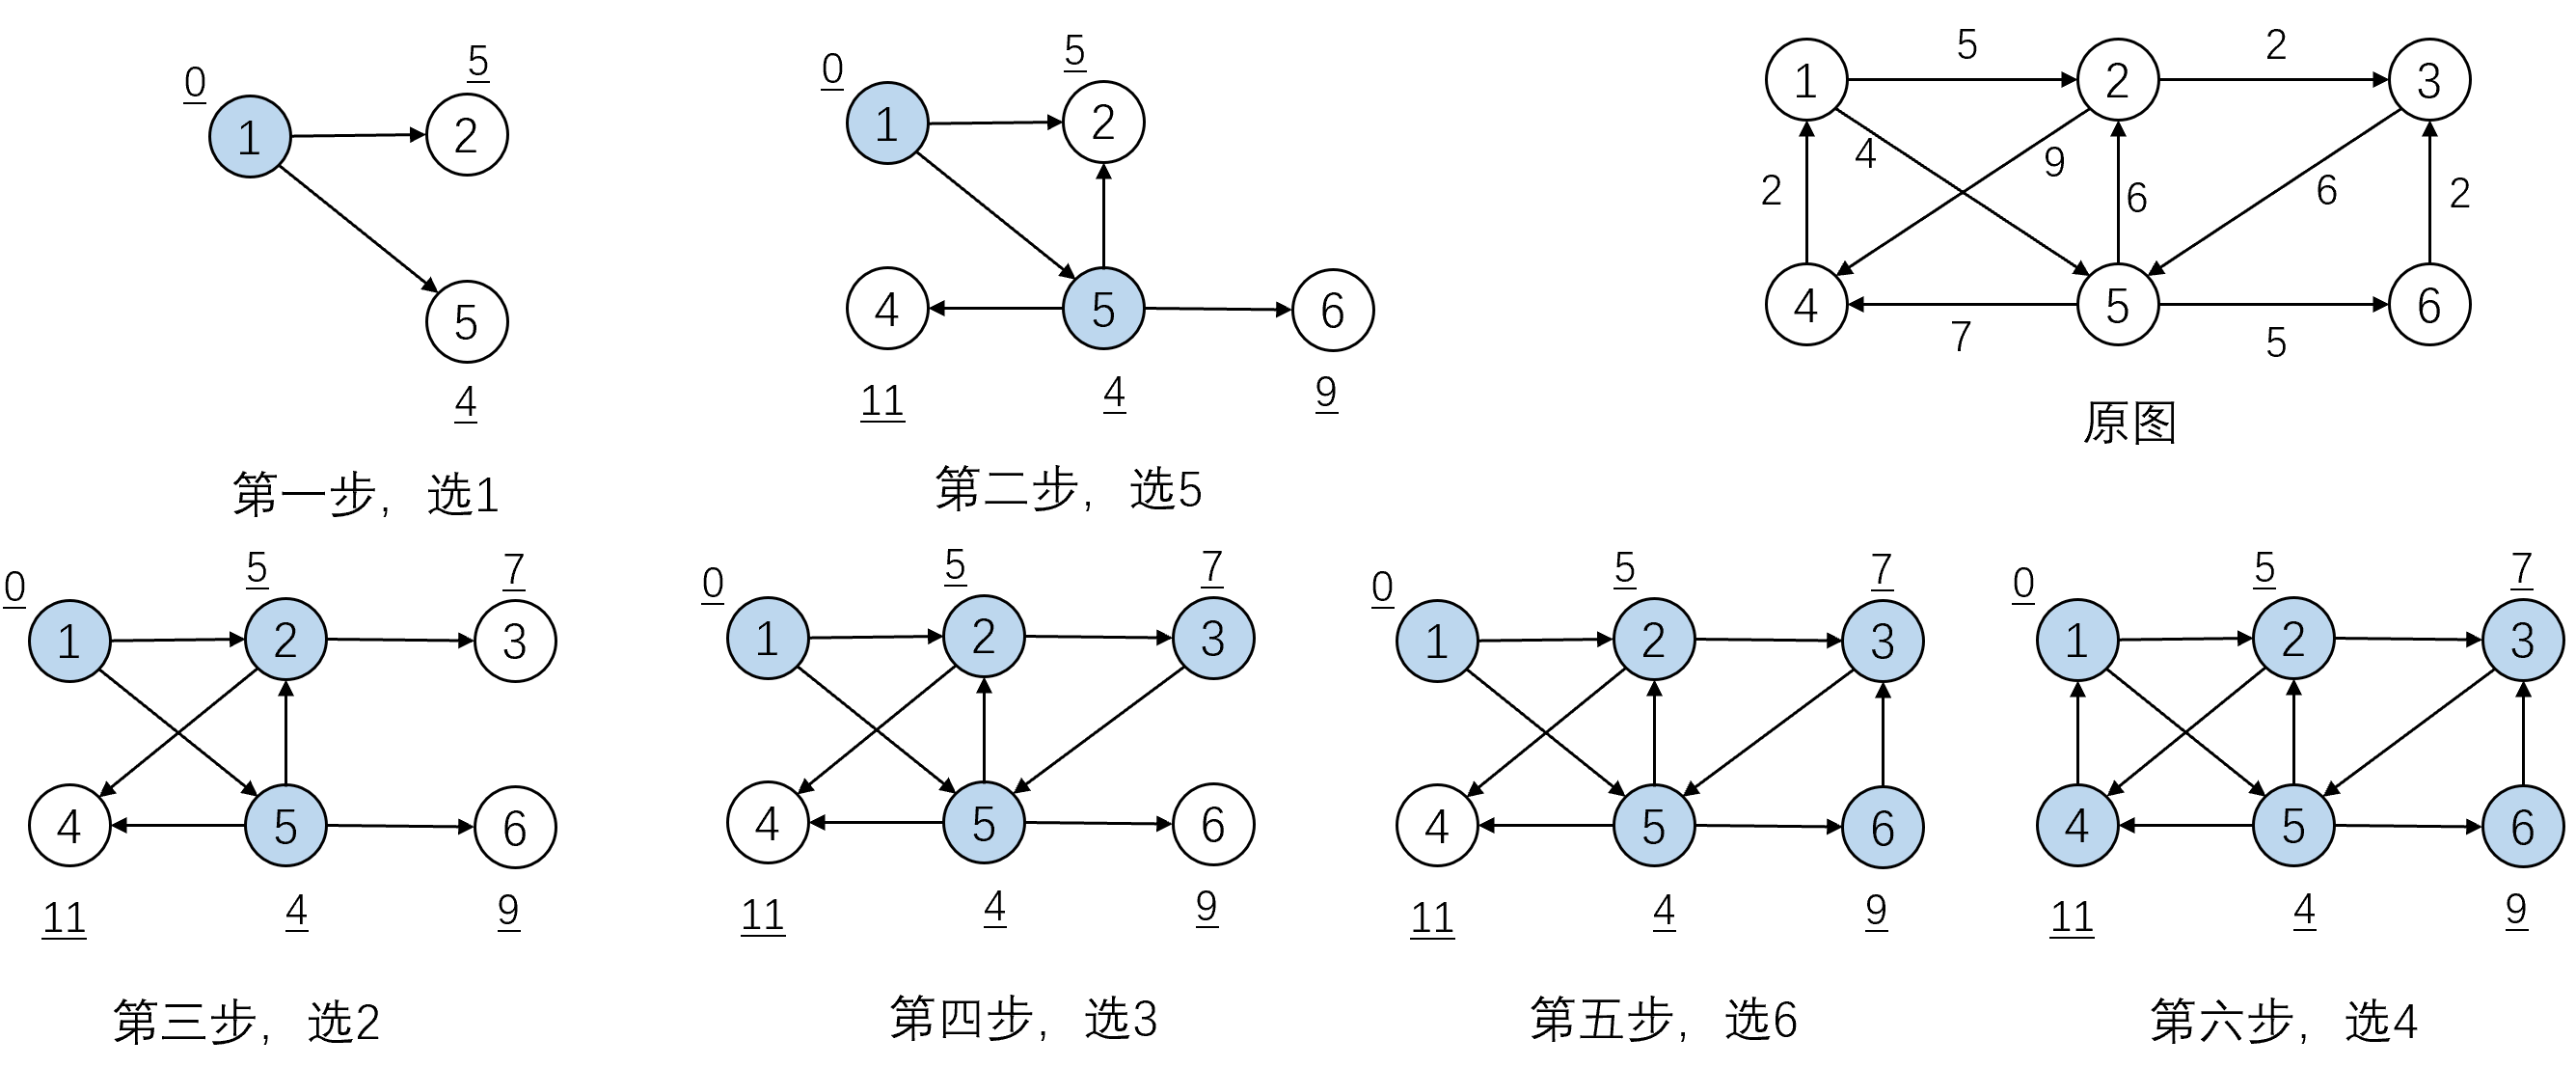
\includegraphics[width=1.02\textwidth]{assets/pics_and_ppts/ch5/习题09，16408最短路径的选点顺序答案图.png}
\end{center}
于是选点顺序是1,5,2,3,6,4，选B。\\

2. 选C。需要注意c到f是有一条边的，别看漏了就行。\\

3. 选C。求解前两个顶点（不包括源点）的最短路径过程如下所示。
\begin{center}
    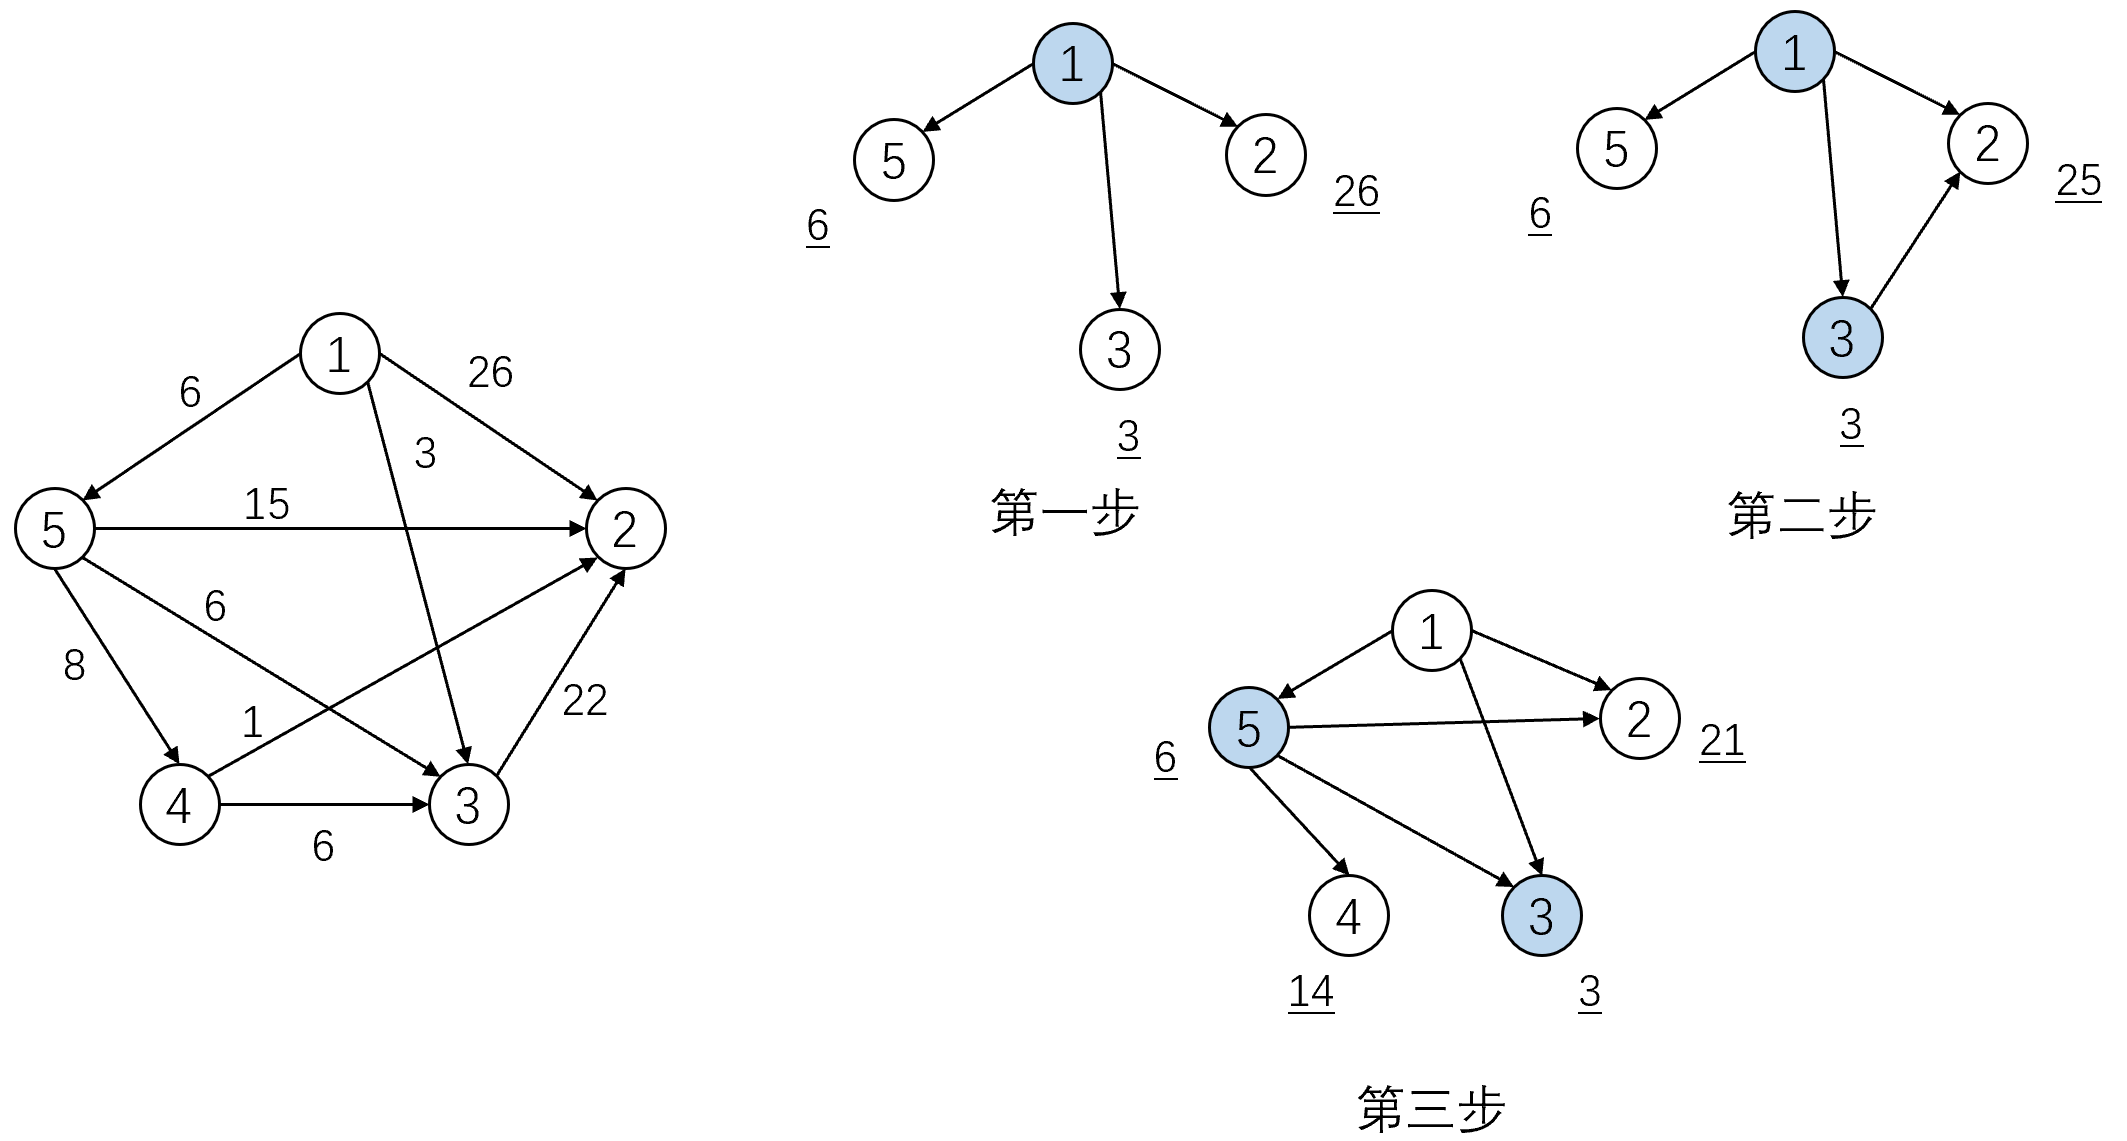
\includegraphics[width=0.90\textwidth]{assets/pics_and_ppts/ch5/习题11，21408迪杰斯特拉dist内容答案图.png}
\end{center}

\vspace{\baselineskip}

4. a）若存在从源点可达的负环，则源点s与任何一个顶点v的最短路径，都可以通过“先走到负环，然后一直绕圈，再走到v”的方式，将最短路径“刷到负无穷”，因此若图中
存在源点可达的负环，通常认为最短路径问题不可解，或者为负无穷；而Bellman-Ford算法可以在图存在负环时给出“不可解”的结论，Dijkstra算法则难以做到这一点。

b）若存在源点可达的负权边，那么迪杰斯特拉算法将失效，求解出可能错误的最短路径；而Bellman-Ford及SPFA算法可以应对存在负权边的图，给出正确的最短路径。

三种算法总结如下：\\

\begin{tabular}{|c|c|c|c|}
    \hline
    \textbf{图的特点} &	\textbf{Dijkstra} &	\textbf{Bellman-Ford} &	\textbf{SPFA}\\
    \hline
    所有边权非负 &	可以 & 可以 & 可以\\
    \hline
    存在负权边，无可达负环 & 不保证正确 & 可以 & 可以 \\
    \hline
    存在可达负权环 & 不保证正确，无法可靠检测 & 可以检测 & 可以检测\\
    \hline
\end{tabular}

\vspace{\baselineskip}

5. 本题意在给大家练习求解最短路径的迪杰斯特拉算法、SPFA算法的代码。显然，我们使用算法求出各顶点的最短路径，返回维火女所在顶点的最短路径即可。
使用迪杰斯特拉算法求解的代码如下：
\begin{cppcode}
    // N 已定义
    struct AdjEdge {
        int u;          // 顶点编号
        int time_cost;  // 花费时间（边权）
    };
    vector<AdjEdge> AdjList[N];    // 已存储邻接表信息 
    char ver_info[N];   // 已存储顶点信息
    // 返回以s为起点到达维火女的房间需要花费的最短时间
    int MinTime(int s) {
        const int inf = 0x3fffffff;
        int cur_mind[N];
        bool solved[N];
        // 记录维火女所在的牢房编号firekeeper_idx，函数最后返回cur_mind[firekeeper_idx]。
        int firekeeper_idx = -1;
        
        // 初始化的过程顺便找一下维火女在哪
        for(int i=0; i<N; i++) {
            cur_mind[i] = inf;
            solved[i] = false;
            if(ver_info[i] == 'T') {
                firekeeper_idx = i;
            }
        }
        cur_mind[s] = 0;

        for(int i=0; i<N-1; i++) {
            // 从尚未求解的顶点中选出一个cur_mind[]最小的顶点v
            int min_curmind = inf;
            int v = -1;
            for(int j=0; j<N; j++) {
                if(cur_mind[j] < min_curmind && !solved[j]) {
                    v = j;
                    min_curmind = cur_mind[j];
                }
            }

            if(v == -1) {
                break;
            }
            solved[v] = true;
            // 已经计算出维火女了，就别再计算其他的了，赶紧去救她吧！
            if(v == firekeeper_idx) {
                return cur_mind[v];
            }

            for(int j=0; j<AdjList[v].size(); j++) {
                int u = AdjList[v][j].u;
                int time_cost = AdjList[v][j].time_cost;
                if(cur_mind[v] + time_cost < cur_mind[u]) {
                    cur_mind[u] = cur_mind[v] + time_cost;
                }
            }
            
        }
        return cur_mind[firekeeper_idx] == inf? -1 : cur_mind[firekeeper_idx];
    }
\end{cppcode}

使用SPFA算法求解的代码如下：
\begin{cppcode}
    // N 已定义
    struct AdjEdge {
        int u;          // 顶点编号
        int time_cost;  // 花费时间（边权）
    };
    vector<AdjEdge> AdjList[N];    // 已存储邻接表信息 
    char ver_info[N];   // 已存储顶点信息
    // 返回以s为起点到达维火女的房间需要花费的最短时间
    int MinTime(int s) {
        const int inf = 0x3fffffff;
        int cur_mind[N];
        bool in_queue[N];
        /* 该场景明确图中无负边，因此无需进行负环
        检测，也就不需要inq_cnt[]数组，但这里还是
        以注释给出，帮助大家再次复习若需要检测负环
        时，代码该怎么写。 */
        // int inq_cnt[N];  
        int firekeeper_idx = -1;
        for(int i=0; i<N; i++) {
            cur_mind[i] = inf;
            in_queue[i] = false;
            // inq_cnt[i] = 0;
            if(ver_info[i] == 'T') {
                firekeeper_idx = i;
            }
        }
        cur_mind[s] = 0;
        queue<int> q;
        q.push(s);
        in_queue[s] = true;
        while(!q.empty()) {
            int v = q.front();
            q.pop();
            in_queue[v] = false;
            for(int i=0; i<AdjList[v].size(); i++) {
                int u = AdjList[v][i].u; 
                int time_cost = AdjList[v][i].time_cost;
                if(cur_mind[v] + time_cost < cur_mind[u]) {
                    cur_mind[u] = cur_mind[v] + time_cost;
                    if(!in_queue[u]) {
                        in_queue[u] = true;
                        q.push(u);
                        // inq_cnt[u] += 1;
                    }

                    // 若可能存在负环，在此处进行负环判断
                    
                }
            }
        }
        return cur_mind[firekeeper_idx] == inf ? -1 : cur_mind[firekeeper_idx];
    }
\end{cppcode}

\vspace{\baselineskip}

6. 

\begin{wrapfigure}{r}{0.22\textwidth}  
    \centering
    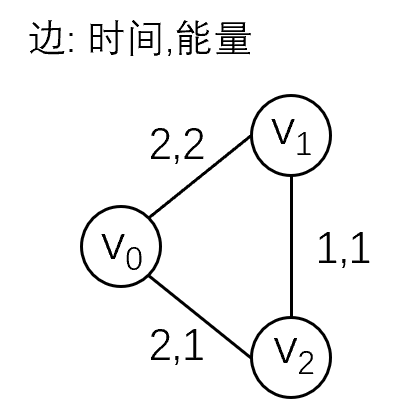
\includegraphics[width=0.80\linewidth]{assets/pics_and_ppts/ch5/习题12营救维火女最短时间、最小能量答案图.png}
\end{wrapfigure}

若使用迪杰斯特拉算法，就要同时记录每个点的当前已知最短时间及对应最短时间路径的最小能量消耗：cur\_mint[i]为j表示顶点i到s的最短时间为j，并且cur\_mine[i]
为k表示顶点i到s的最短时间路径下，最小消耗为k。

而且每次“选点”时，就不能只选择时间花费最小的，而是要选的时间花费最小的条件下，能量消耗最小的那个点。如图，
以$v_0$为起点，若直接选择了$v_1$，则会得到错误答案。在更新时类似，当时间更短，或时间相等但能量消耗更少时更新即可。代码如下：

\begin{cppcodeHighlight}[11-12,17-18,29-30,32-39,53-59]
    // N 已定义
    struct AdjEdge {
        int u;          
        int time_cost;      // 花费时间
        int energy_cost;    // 和敌人战斗需要消耗的能量值
    };
    vector<AdjEdge> AdjList[N];    // 已存储邻接表信息 
    char ver_info[N];   // 已存储顶点信息
    // 返回以s为起点到达维火女的房间花费时间最短的路径中，消耗能量最少的那条路径所消耗的能量值
    int MinEnergyCost(int s) {
        int cur_mint[N];    // 当前已知的各顶点最短时间
        int cur_mine[N];    // 对应最短时间路径中的最小能量消耗
        bool solved[N];
        const int inf = 0x3fffffff;
        int firekeeper_idx = -1;
        for(int i=0; i<N; i++) {
            cur_mint[i] = inf;
            cur_mine[i] = inf;
            solved[i] = false;
            if(ver_info[i] == 'T') {
                firekeeper_idx = i;
            }
        }

        cur_mint[s] = 0;
        cur_mine[s] = 0;
        
        for(int i=0; i<N-1; i++) {
            int min_timecost = inf;
            int min_energycost = inf;
            int v = -1;
            for(int j=0; j<N; j++) {
                if(!solved[j] && (cur_mint[j] < min_timecost || 
                    cur_mint[j] == min_timecost && cur_mine[j] < min_energycost) 
                ) {
                    min_timecost = cur_mint[j];
                    min_energycost = cur_mine[j];
                    v = j;
                }
            }

            if(v == -1) {
                break;
            }
            solved[v] = true;
            if(v == firekeeper_idx) {
                break;
            }
            for(int j=0; j<AdjList[v].size(); j++) {
                int u = AdjList[v][j].u;
                int time_cost = AdjList[v][j].time_cost;
                int energy_cost = AdjList[v][j].energy_cost;
                if(cur_mint[v] + time_cost < cur_mint[u]) {
                    cur_mint[u] = cur_mint[v] + time_cost;
                    cur_mine[u] = cur_mine[v] + energy_cost;
                }
                else if(cur_mint[v] + time_cost == cur_mint[u] && cur_mine[v] + energy_cost < cur_mine[u]) {
                    cur_mine[u] = cur_mine[v] + energy_cost;
                }
            }
        }
        return cur_mine[firekeeper_idx] == inf ? -1 : cur_mine[firekeeper_idx];
    }
\end{cppcodeHighlight}
事实上本题可以从另一个角度去理解：有些时候我们可能在求时间最短的最短路径，有些时候求路程最短，有些时候求花费最少......，时间、路程、花费的大小比较规则就是比数值。

而本题“时间”和“能量”共同组成了某个东西，拟叫它“代价”好了，那么本题其实就是在求“代价”最短的最短路径。只不过“代价”有着不太一样的大小比较规则：对于两个表示
“代价”的变量a和b，

1）a“小于”b定义为：a的时间比b小，或a与b时间相等并且a的能量比b小；

2）a“等于”b定义为：a与b的时间、能量完全相等；

3）a“大于”b定义为：a的时间比b大，或a与b时间相等并且a的能量比b大；

因此，我们在每次“选点”时，就像要以时间、路程、花费等为标尺选出最小的一样，本题我们就是在选出“代价”最小的；在更新时，是在比较“代价”的大小，若以v为中介，
能够使得u的“代价”更小，则更新u。这也从另一个角度理解了以上代码实现。

同时，通过C++的运算符重载功能，我们可以对这种结构体的大小比较进行定义：
\begin{cppcode}
    struct cost {
        int time ;
        int energy;
        // 定义cost类型对象的“<”比较规则
        bool operator < (const cost& other) const {
            return this->time < other.time ||
                (this->time == other.time && this->energy < other.energy);
        }

        // 定义两个代价相加规则
        cost operator + (const cost& other) const {
            cost ret;
            ret.time = this->time + other.time;
            ret.energy = this->energy + other.energy;
            return ret;
        }
    };
    cost cur_minc[N];   // 这一个数组就包含了cur_mint和cur_mine的功能
\end{cppcode}
然后每次“选点”时：
\begin{cppcode}
    cost min_cost;
    min_cost.time = inf;
    min_cost.energy = inf;
    int v = -1;
    for(int j=0; j<N; j++) {
        if(!solved[j] && cur_minc[j] < min_cost ) {
            min_cost = cur_minc[j];
            v = j;
        }
    }
    ...
\end{cppcode}
更新时：
\begin{cppcode}
    for(int j=0; j<AdjList[v].size(); j++) {
        int u = AdjList[v][j].u;
        cost c;
        c.time = AdjList[v][j].time_cost;
        c.energy = AdjList[v][j].energy_cost;
        if(cur_minc[v] + c < cur_minc[u]) {
            cur_minc[u] = cur_minc[v] + c;
        }
    }
\end{cppcode}
这种运算符重载规则，可以在我们使用C++标准库提供的排序函数std::sort()时来自定义一些排序规则，我们将在\ref{minisec:Kruskal算法实现}节（
第\pageref{minisec:Kruskal算法实现}页）中看到。



\end{exerciseanswer}%%%%%%%%%%%%%%%%%%%%%%%%%%%%%%%%%%%%%%%%%%%%%%%%%%%%%%%%%%%%%%%%%%%%%%%%%%%%%%%%%%%%%%%%%%%%%%%%%%%%%%%%%%%%%%%%%%%%%%%%%%%%%%%%%%%%%%%%%
你成功营救出了维火女，你们一同回到大陆中，继续冒险。她手中正是那樱花之泪。
\section{最小生成树}
王国的指挥官们解决了最短路径问题之后，又提出了一个新的问题：目前据点之间通信只能通过信使传递，他们希望在据点之间铺设通信线缆，使得信息可以顺着线缆迅速传递。
指挥官们认为，没有必要在任意两个据点之间都铺设线缆，而是只要能够保证任意两个据点之间都可以通过线缆连通即可。
这样一来，即使信息需要经过其他据点中转，也能实现整个王国的线缆通信。

然而，铺设线缆需要耗费大量资源。不同据点之间铺设线缆所需的成本各不相同。指挥官们希望找到一种方案：既能保证所有据点都连通，又能使铺设线缆的总成本尽可能低。
应该如何设计这样的方案呢？这其实就是\term{最小生成树}的问题：


给定一个\uline{连通的}无向带权图 \(G=(V,E)\)，如果从图中选择若干条边，使得所有顶点连通且不存在环，
那么图的所有顶点及这些边构成的子图就是原图的一棵\term{生成树}。在所有生成树中，边权总和最小的生成树称为\term{最小生成树（Minimum Spanning Tree，MST）}。\\

对此问题，格佛莱指出：初始时随意选择一个顶点s，然后选择依附于s的边权最小的一条边，将该边与相连顶点“收进来”，
此时，当前的生成树中就已经有了2个顶点。然后，继续选择能够连通这2个顶点与其他顶点的一条边权最小的边，并将该边与相连的顶点“收进来”，生成树中就有了3
个顶点。重复这个操作，直至所有顶点都被“收进来”。这样做，得到的生成树中的所有边，一定是使得顶点连通的所有边的选集中权值之和最小的$N-1$条边。
如图\ref{fig:Prim算法道理说明}所示，使得三个顶点连通，可选的边集有$\{e_0, e_1\}$、$\{e_0, e_2\}$以及$\{e_1, e_2\}$，权值之和最小的一定是$\{e_0, e_1\}$。

因此得到的树一定就是最小生成树。这就是\term{Prim（普里姆）算法}的核心思想。
\begin{figure}[htbp]
    \centering
    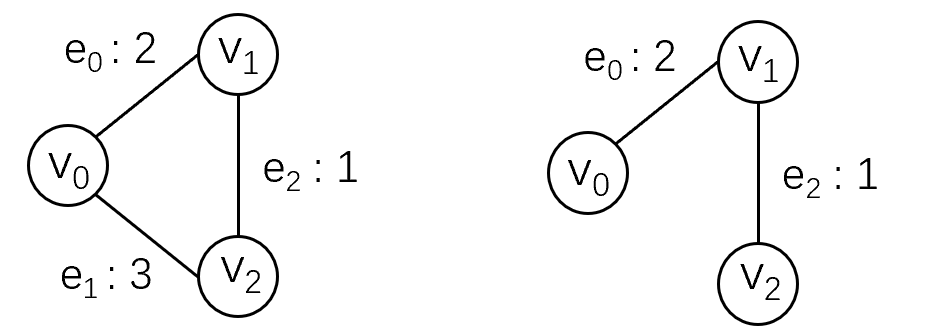
\includegraphics[width=0.50\textwidth]{assets/pics_and_ppts/ch5/24Prim算法道理说明.png}
    \caption{}
    \label{fig:Prim算法道理说明}
\end{figure}

可以看出，对于Prim算法，我们需要动态维护当前生成树以及尚未收入的所有顶点到当前生成树的最小代价。详细实现如下。
\subsection{Prim（普里姆）算法}
设无向连通图$G=(V,E)$，Prim算法的过程如下：设置集合S保存已经收入当前的生成树中的顶点，cur\_mind[]保存各未收入顶点到集合S的最小代价。
初始时随意收入一个顶点s（即S=\{s\}），令与s邻接的所有顶点的cur\_mind[]为相应边权，令其他所有顶点的cur\_mind[]为正无穷。然后执行$N-1$次以下两个步骤：
\begin{enumerate}
    \item 从集合V-S（还未收入当前生成树的顶点集）中选择距离集合S代价最小的一个顶点（即cur\_mind[]最小）u，将u加入S，并将u以及这条边加入当前生成树中。
    \item 对于 u 的每个未被收入S的邻接点 v，执行 
    \[
        cur\_mind[v] = min(cur\_mind[v], cost(u, v))
    \] 
    即如果通过 u 到达 v 的代价比原来记录的更小，则更新 cur\_mind[v]。
\end{enumerate}
可以看到这个过程与迪杰斯特拉算法非常像，迪杰斯特拉算法是每次选择与\uline{源点s}最近的顶点，而Prim算法是选择与\uline{已有生成树S}最近的顶点。注意：Prim算法中，
cur\_mind[v]记录的并不是顶点v到源点s的最短距离，而是顶点v到集合S的最短距离，即v到S中的所有顶点的距离中最小的那个。

我们以图\ref{fig:Prim算法过程演示} a）所示的图，演示一遍Prim算法的过程：

1）任选一个点，假设选A，收入最小生成树，更新A的邻接点B和C的cur\_mind[]，如b）所示；此时集合S为\{A\}。图中带下划线的数字表示还未收入生成树的各个顶点
距集合S的最小代价（最短距离）；图中虚线表示该顶点最近是被哪条边所更新的，收入该顶点时沿着虚线就能找到边。

\begin{figure}[htbp]
    \centering
    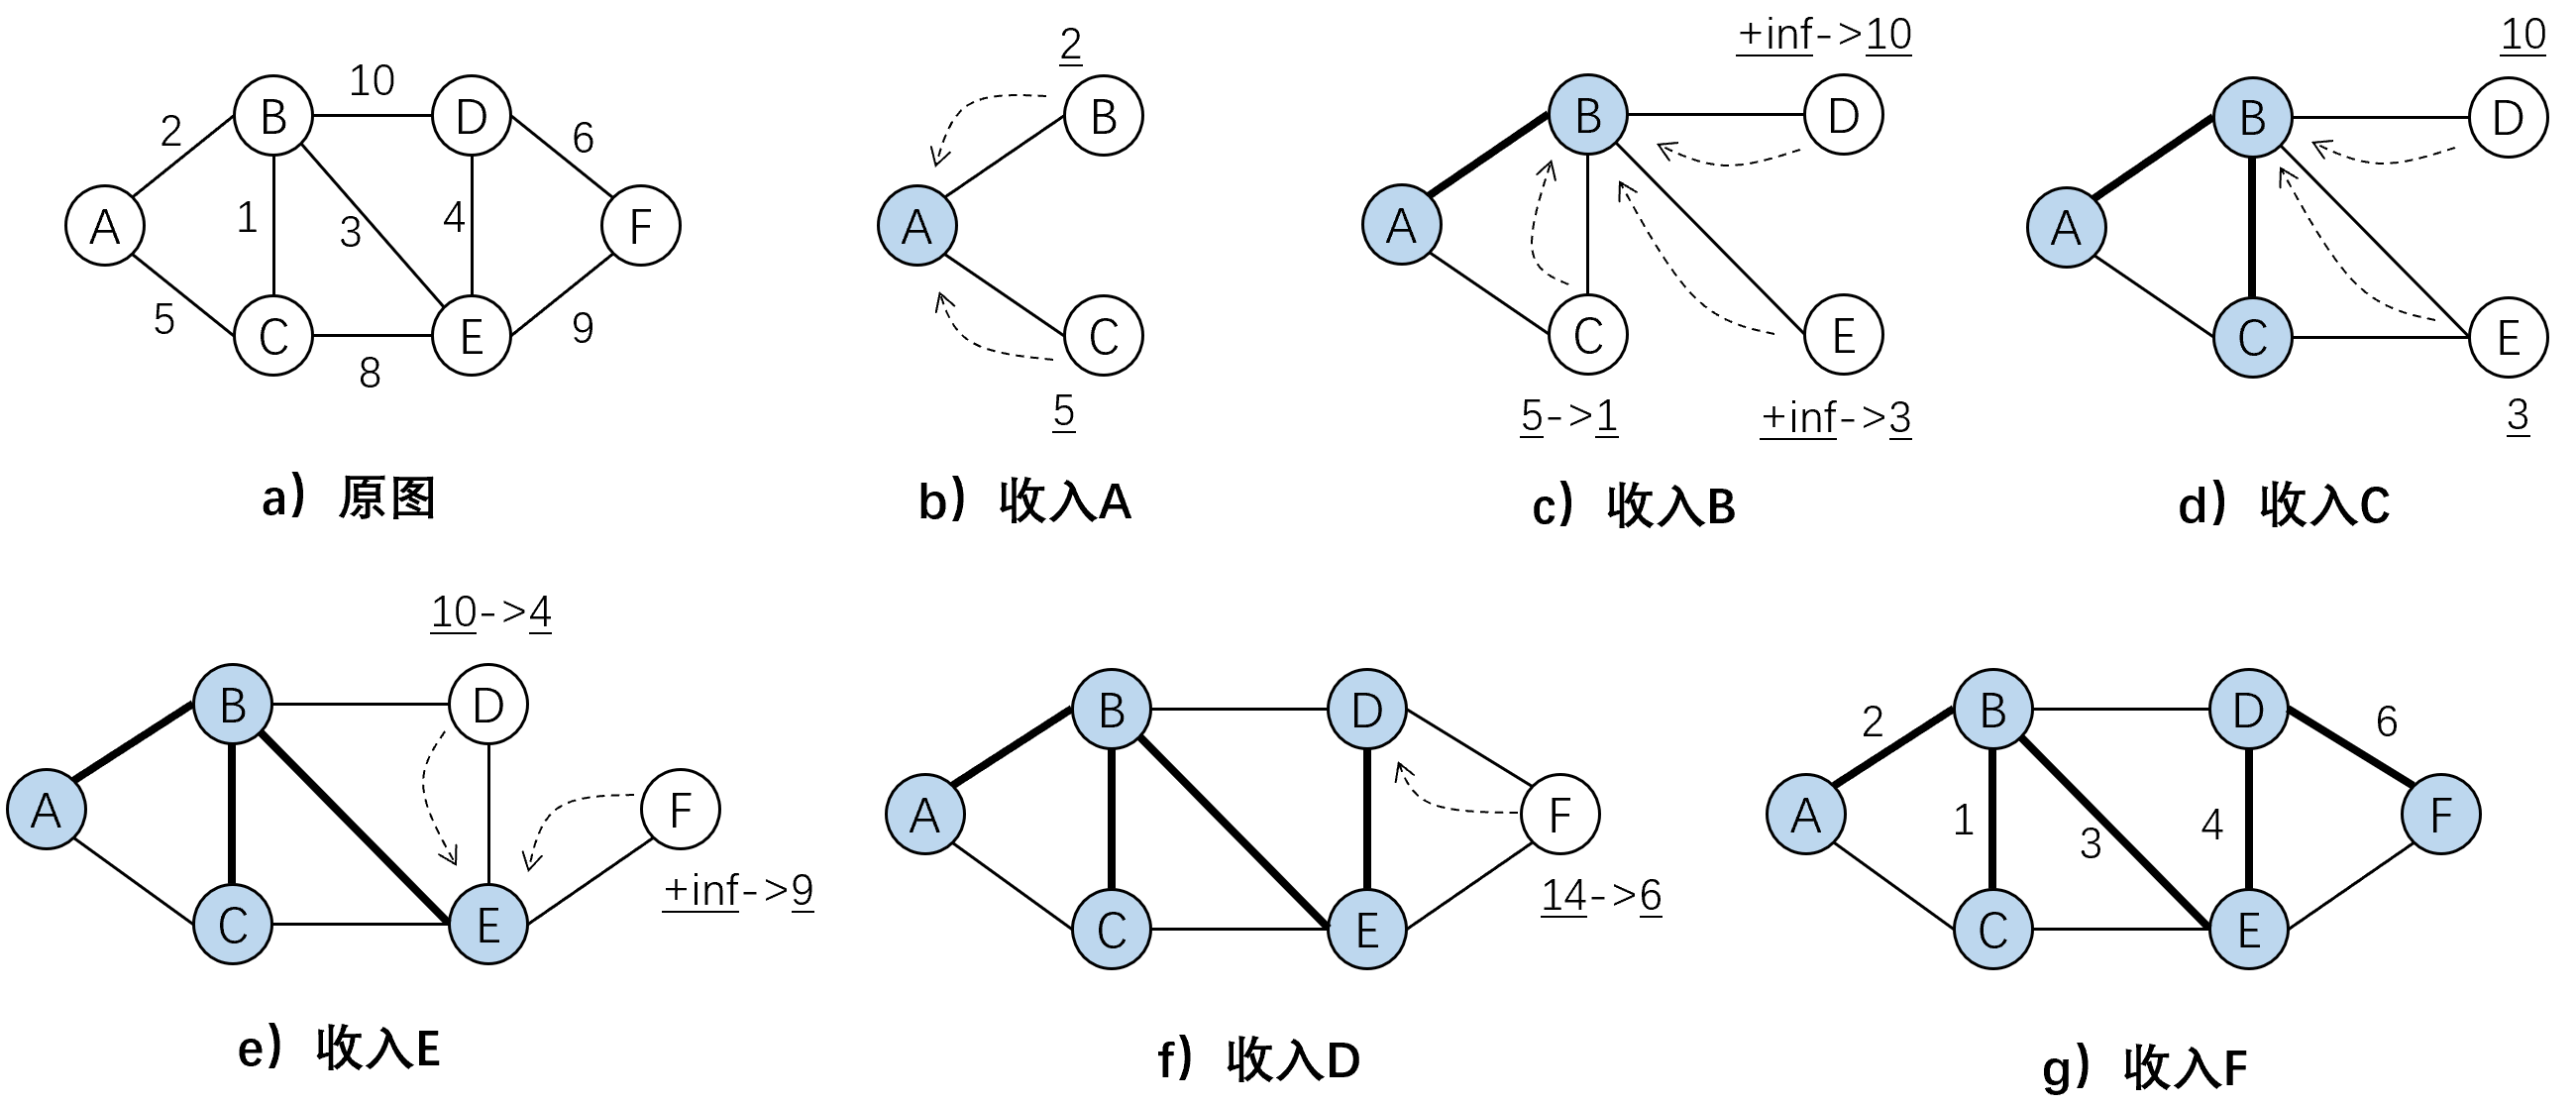
\includegraphics[width=1.01\textwidth]{assets/pics_and_ppts/ch5/25Prim算法过程演示.png}
    \caption{Prim算法过程演示}
    \label{fig:Prim算法过程演示}
\end{figure}

2）未收入的顶点中，到集合S代价最小（最近）的顶点是B，于是收入B，如c）所示，收入B后，
由于 $cur\_mind[C] = 5 < cost(B, C) = 1$，也就是说对于新的集合S=\{A, B\}，C到B的距离更小了，于是更新C到集合S的距离为1。类似地，更新cur\_mind[E]为3、
cur\_mind[D]为10。

3）未收入的顶点中，到集合S代价最小（最近）的顶点是C，于是收入C，如d）所示，并且对于C的邻接点E，由于$cur\_mind[E] = 3 < cost(C, E) = 8$，因此无需更新。

4）收入E，然后更新D、F，如e）所示；

5）收入D，然后更新F，如f）所示；

6）收入F，所有顶点均已被收入生成树，此时得到的即是最小生成树，各个边的权值之和即是最小代价：2 + 1 + 3 + 4 + 6 = 16。\\



\subsection{Kruskal（克鲁斯卡尔）算法}
\label{subsec:Kruskal算法}
指挥官麦丽凯给出了一种完全不同的思路：她不喜欢一步一步细致、缜密地规划，而是将注意力放眼全局。
麦丽凯指出：初始时，没有任何顶点和边被收入生成树，将图看成是$N$个割裂的顶点构成了$N$个连通块。首先挑选整个图中边权最小的边，将它以及它连通的两个顶点
加入生成树，连通块的数量便还剩$N-1$个。此后，每次选择剩余边中权值最小的，若它所连接的两个顶点处在不同连通块，则将他们连通并收入生成树，直至所有顶点均已连通。

该策略显然是正确的。因为如果两个连通块之间存在一条权值最小的边，那么最优解是一定要包含这条边的。
这种放眼全局，通过不断地选择边权最小的边将不同连通块合并的策略，这就是\term{Kruskal（克鲁斯卡尔）算法}的核心思想。


具体来说，设无向连通图$G=(V,E)$有$N$个顶点，Kruskal算法的过程如下：
将图看成是$N$个割裂的顶点构成了$N$个连通块。然后反复按边权从小到大检查所有还未被收入生成树的边，
若被检查的边所连接的两个顶点不在同一个连通块中，则将他们连通，并收入生成树，否则跳过，继续检查下一条边。
如此重复，直至所有顶点均已连通；

我们以\ref{fig:Kruskal算法过程演示} a）所示的图演示一遍Kruskal算法的过程。

1）所有边中权值最小的是连接BC的边（为1），将其收入，如b）所示，此时B、C已被连通；

2）此时剩余所有边中，边权最小的是连接A、B的边（为2），由于A、B此时不在相同的连通块，因此将他们收入生成树，此时A、B、C已被连通，如c）所示；

\begin{figure}[htbp]
    \centering
    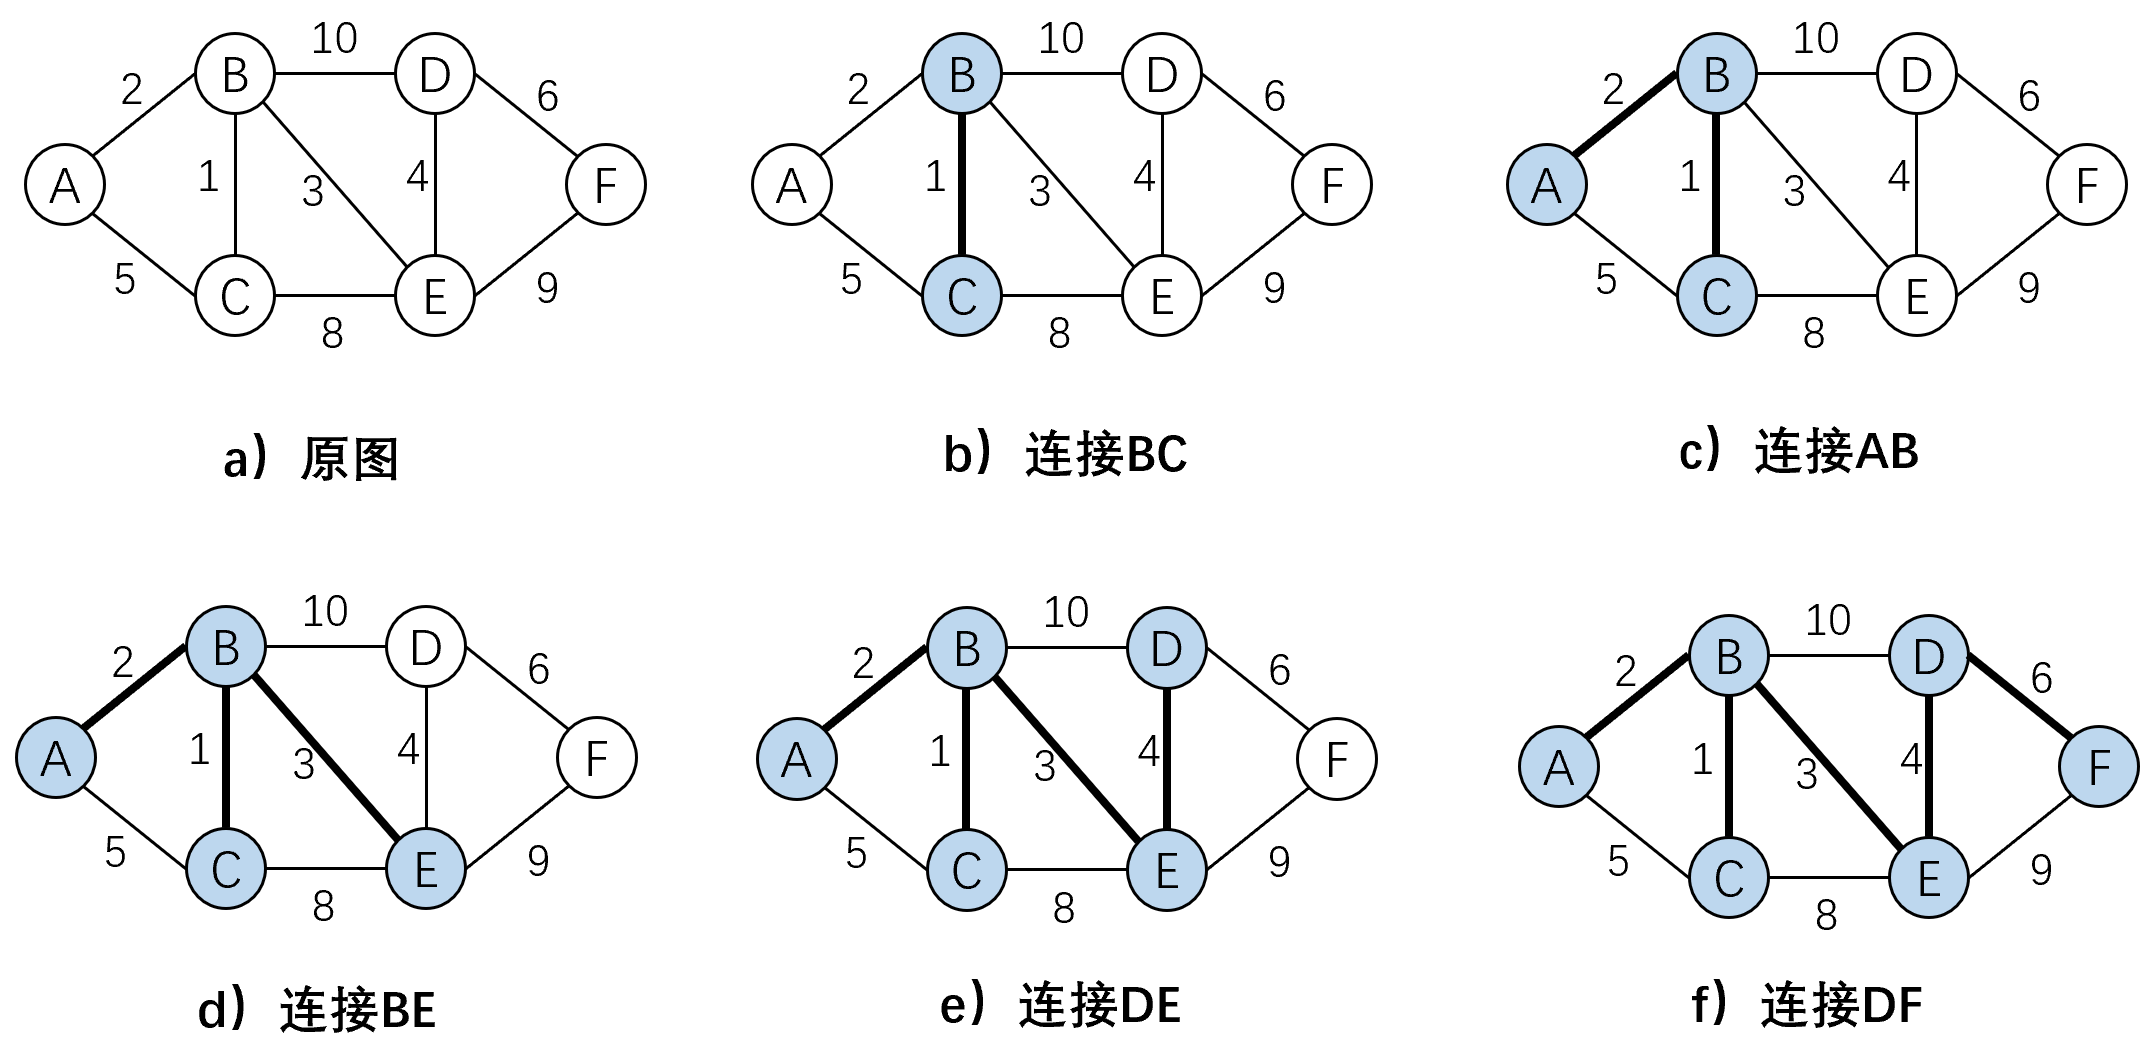
\includegraphics[width=0.95\textwidth]{assets/pics_and_ppts/ch5/26Kruskal算法过程演示.png}
    \caption{Kruskal算法过程演示}
    \label{fig:Kruskal算法过程演示}
\end{figure}

3）此时剩余所有边中，边权最小的是连接B、E的边（为3），由于B、E此时不在相同的连通块，因此将他们收入生成树，此时A、B、C、E已被连通，如d）所示；

4）将D收入生成树，此时A、B、C、E、D已被连通，如e）所示；

5）剩余所有边中，边权最小的是连接A、C的边（为5），但A、C已经处于同一个连通块，因此跳过，继续检查下一条边；

6）剩余所有边中，边权最小的是连接D、F的边（为6），并且D、F处在不同的连通块，于是将它们收入生成树，如f）所示，此时所有顶点均已被连通，算法结束。可以看到，
在这个图的例子中，Kruskal算法得到了与Prim算法相同的最小生成树。

\subsection{算法实现}
\minisection{Prim算法的实现}
Prim算法的代码与Dijkstra算法非常相似。以邻接表为例，Prim算法的实现如下所示（高亮部分是与Dijkstra的区别部分）：
\begin{cppcodeHighlight}[15,33,39-40]
    struct EdgeInfo {
        int u;
        int weight;
    };
    vector<EdgeInfo> AdjList[N];
    const int inf = 0x3fffffff;
    bool solved[N]; // 已初始化为false
    int cur_mind[N];    // 已初始化为inf
    int Pre[N];     // 已初始化为-1

    // 返回生成树的最小代价。
    int Prim(int s) {
        cur_mind[s] = 0;
        // min_cost用于累加生成树的最小代价，算法返回它
        int min_cost = 0;
        // 为了代码简洁，将收入s的操作放在循环里了，因此要做N次循环
        for(int i=0; i<N; i++) {
            int v = -1;
            int min_curmind = inf;
            for(int j=0; j<N; j++) {
                if(!solved[j] && cur_mind[j] < min_curmind) {
                    min_curmind = cur_mind[j];
                    v = j;
                }
            }

            // 图不连通
            if(v == -1) {
                return -1;
            }
            solved[v] = true;
            // 累加代价
            min_cost += cur_mind[v];
            
            for(int j=0; j<AdjList[v].size(); j++) {
                int u = AdjList[v][j].u;
                int weight = AdjList[v][j].weight;
                // 新加入集合的v，能使的u到集合的距离更小
                if(weight < cur_mind[u]) {
                    cur_mind[u] = weight;
                    Pre[u] = v;
                }
            }
        }
        return min_cost;
    }
\end{cppcodeHighlight}
若需要知道这棵最小生成树“长什么样”，则可以在每次选出顶点 v 时，打印出 Pre[v] 和 v，它们即构成了最小生成树中的一条边。同时可以看出，
与迪杰斯特拉算法类似，“选点”的过程同样可以通过堆优化。\\


\minisection{2.Kruskal算法实现}
Kruskal算法需要每次选择边权最小的边，若每次遍历邻接表或邻接矩阵进行“选边”，代价显然无法接受。因此，要实现Kruskal算法，通常需要将所有边按边权排序，
排好序后每次按顺序选择即可。这里为大家引入C++中的标准库sort函数。

\begin{cppcode}
    struct EdgeInfo {
        int u,v;
        int weight;
        // 定义两个EdgeInfo结构体的“<”比较规则
        bool operator < (const EdgeInfo& other) {
            return this->weight < other.weight;
        }
    };
    EdgeInfo edges[M];  // 假设已经存储了图G中所有边的信息
    
    
    int Kruskal() {
        // 按照EdgeInfo的“<”比较规则，对edges数组进行排序。
        std::sort(edges, edges+M);
        // ...
    }
\end{cppcode}

通过上面的代码，就将edges这个数组按照其元素weight的大小关系，排成了一个从小到大的有序数组。
关于结构体的比较规则定义、std::sort的使用请参见第\pageref{sec:为结构体定义比较规则、std::sort()的使用}页。



Kruskal算法选边时，需要判断两个顶点是否在同一个连通块中，若不在，需要将两个连通块合并，这正是并查集提供的功能！我们这里直接使用\ref{sec:并查集}节中提供的
并查集的Find与Union操作。若将所有边遍历一轮之后，收入生成树的边的数量不足$N-1$，说明图不连通。可以写出Kruskal的代码如下：
\begin{cppcode}
    int Kruskal() {
        // 按照EdgeInfo的“<”比较规则，对edges数组进行排序。
        std::sort(edges, edges+M);
        // 要返回的生成树最小代价
        int min_cost = 0;
        // 已收进来的边的数量
        int edgenum_in_tree = 0;
        int father[N];
        for(int i=0; i<N; i++) {
            father[i] = i;
        }

        // 遍历所有边
        for(int i=0; i<M; i++) {
            int u = edges[i].u;
            int v = edges[i].v;
            int u_id = Find(father, u);
            int v_id = Find(father, v);
            // 这条边连接的u、v不在同一个集合
            if(u_id != v_id) {
                Union(father, u, v);
                min_cost += edges[i].weight;
                // cout << “选择了一条边u->v”
                edgenum_in_tree += 1;
            }
        }
        /* 原图不连通，不存在包含所有顶点的生成树。*/
        if(edgenum_in_tree < N-1) {
            return -1;
        }
        return min_cost;
    }
\end{cppcode}



